\section{Experiments}\label{sec:CDSV}







% \begin{figure}[t]
%   \centering
%    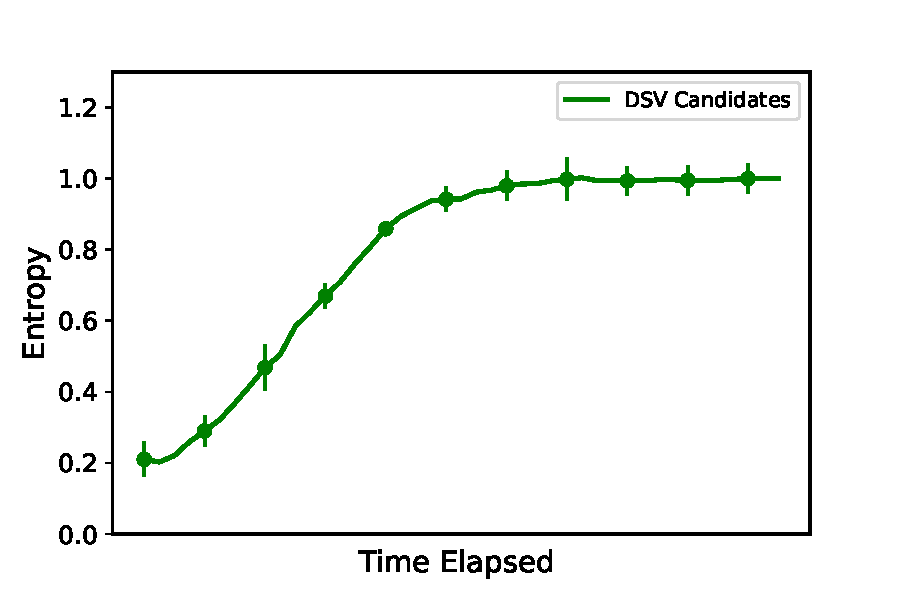
\includegraphics[width=0.8\linewidth]{./figure/Entropy_DSV.pdf}
%    \caption{Illustration of entropy change with DSV candidates: We utilized DeepKKT conditions in the selection of DSVs. As training progresses, entropy increases, \ie the DSVs move toward the decision boundary.}
%    \label{fig:lambda_entropy}
% \end{figure}
% \begin{figure}[t]
%   \centering
%    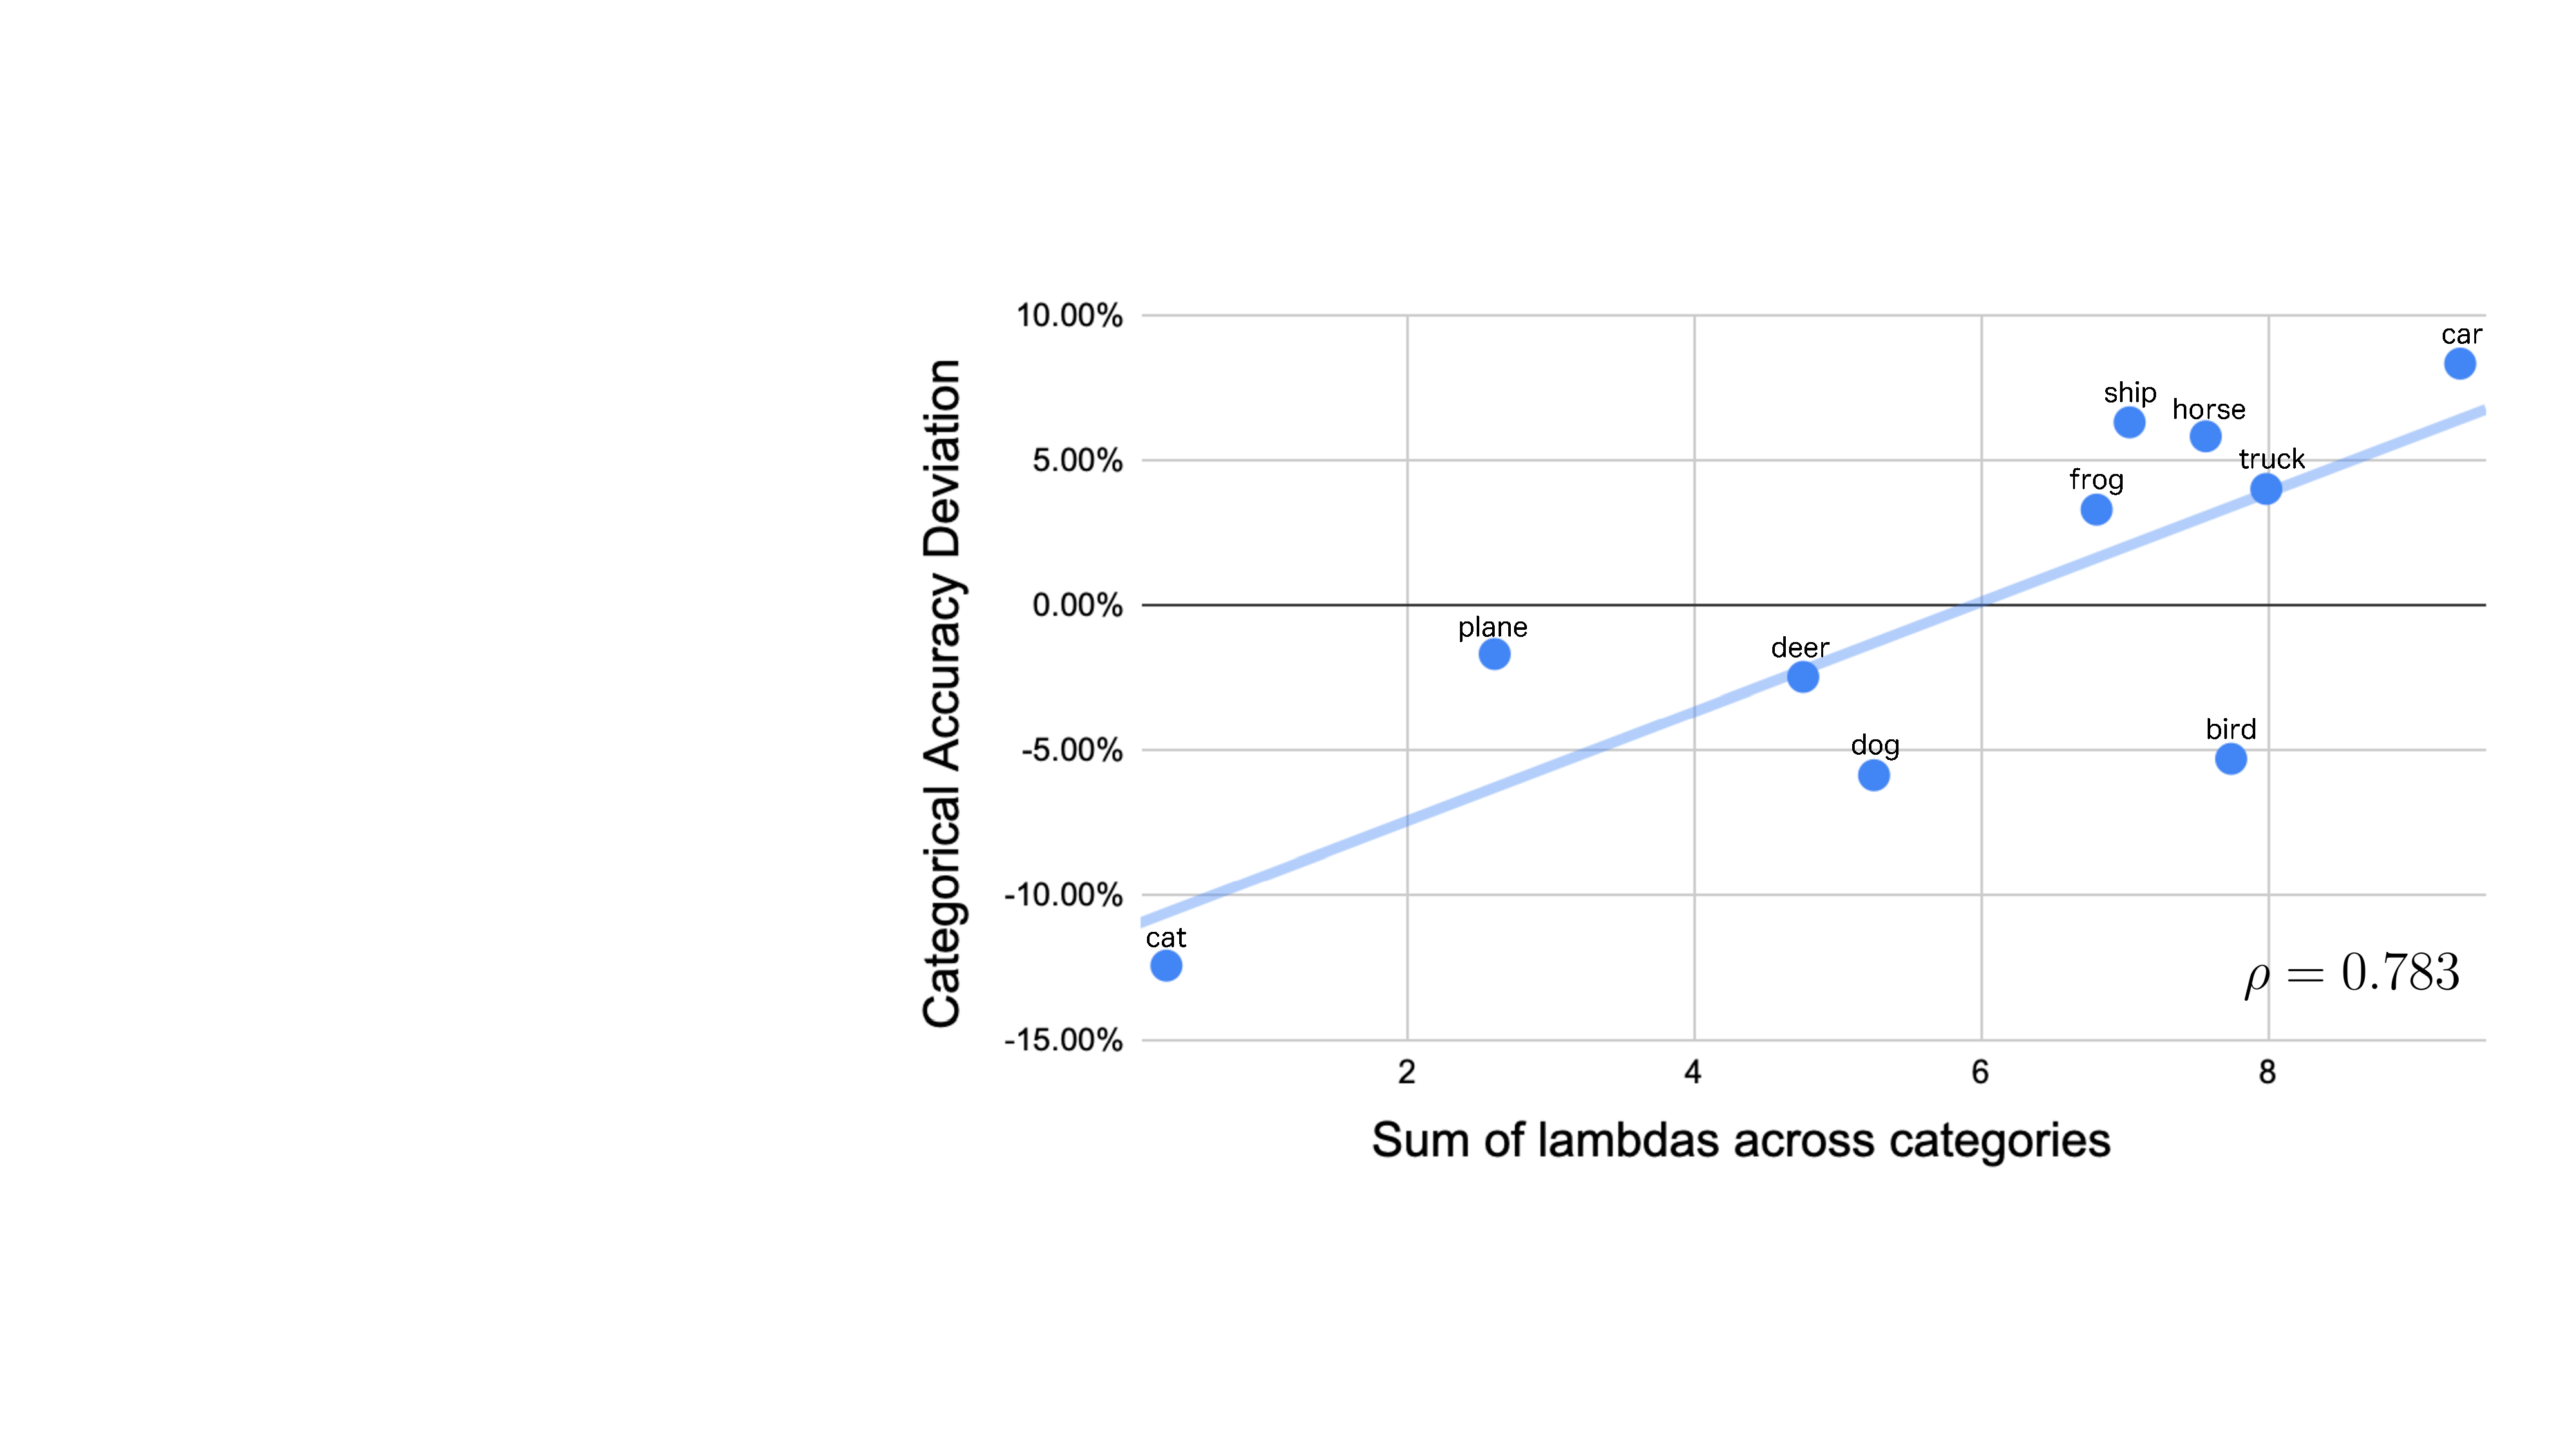
\includegraphics[width=1.0\linewidth]{./figure/pearson.pdf}
%    \vspace{-7mm}
%    \caption{\nj{Correlation between the classwise mean test accuracy versus the sum of $\lambda$'s for training samples belonging to each class. Here, $\rho$  represents the Pearson correlation coefficient.}}
%    \label{fig:correlation}
% \end{figure}
% \begin{figure}[t]
%   \centering
%    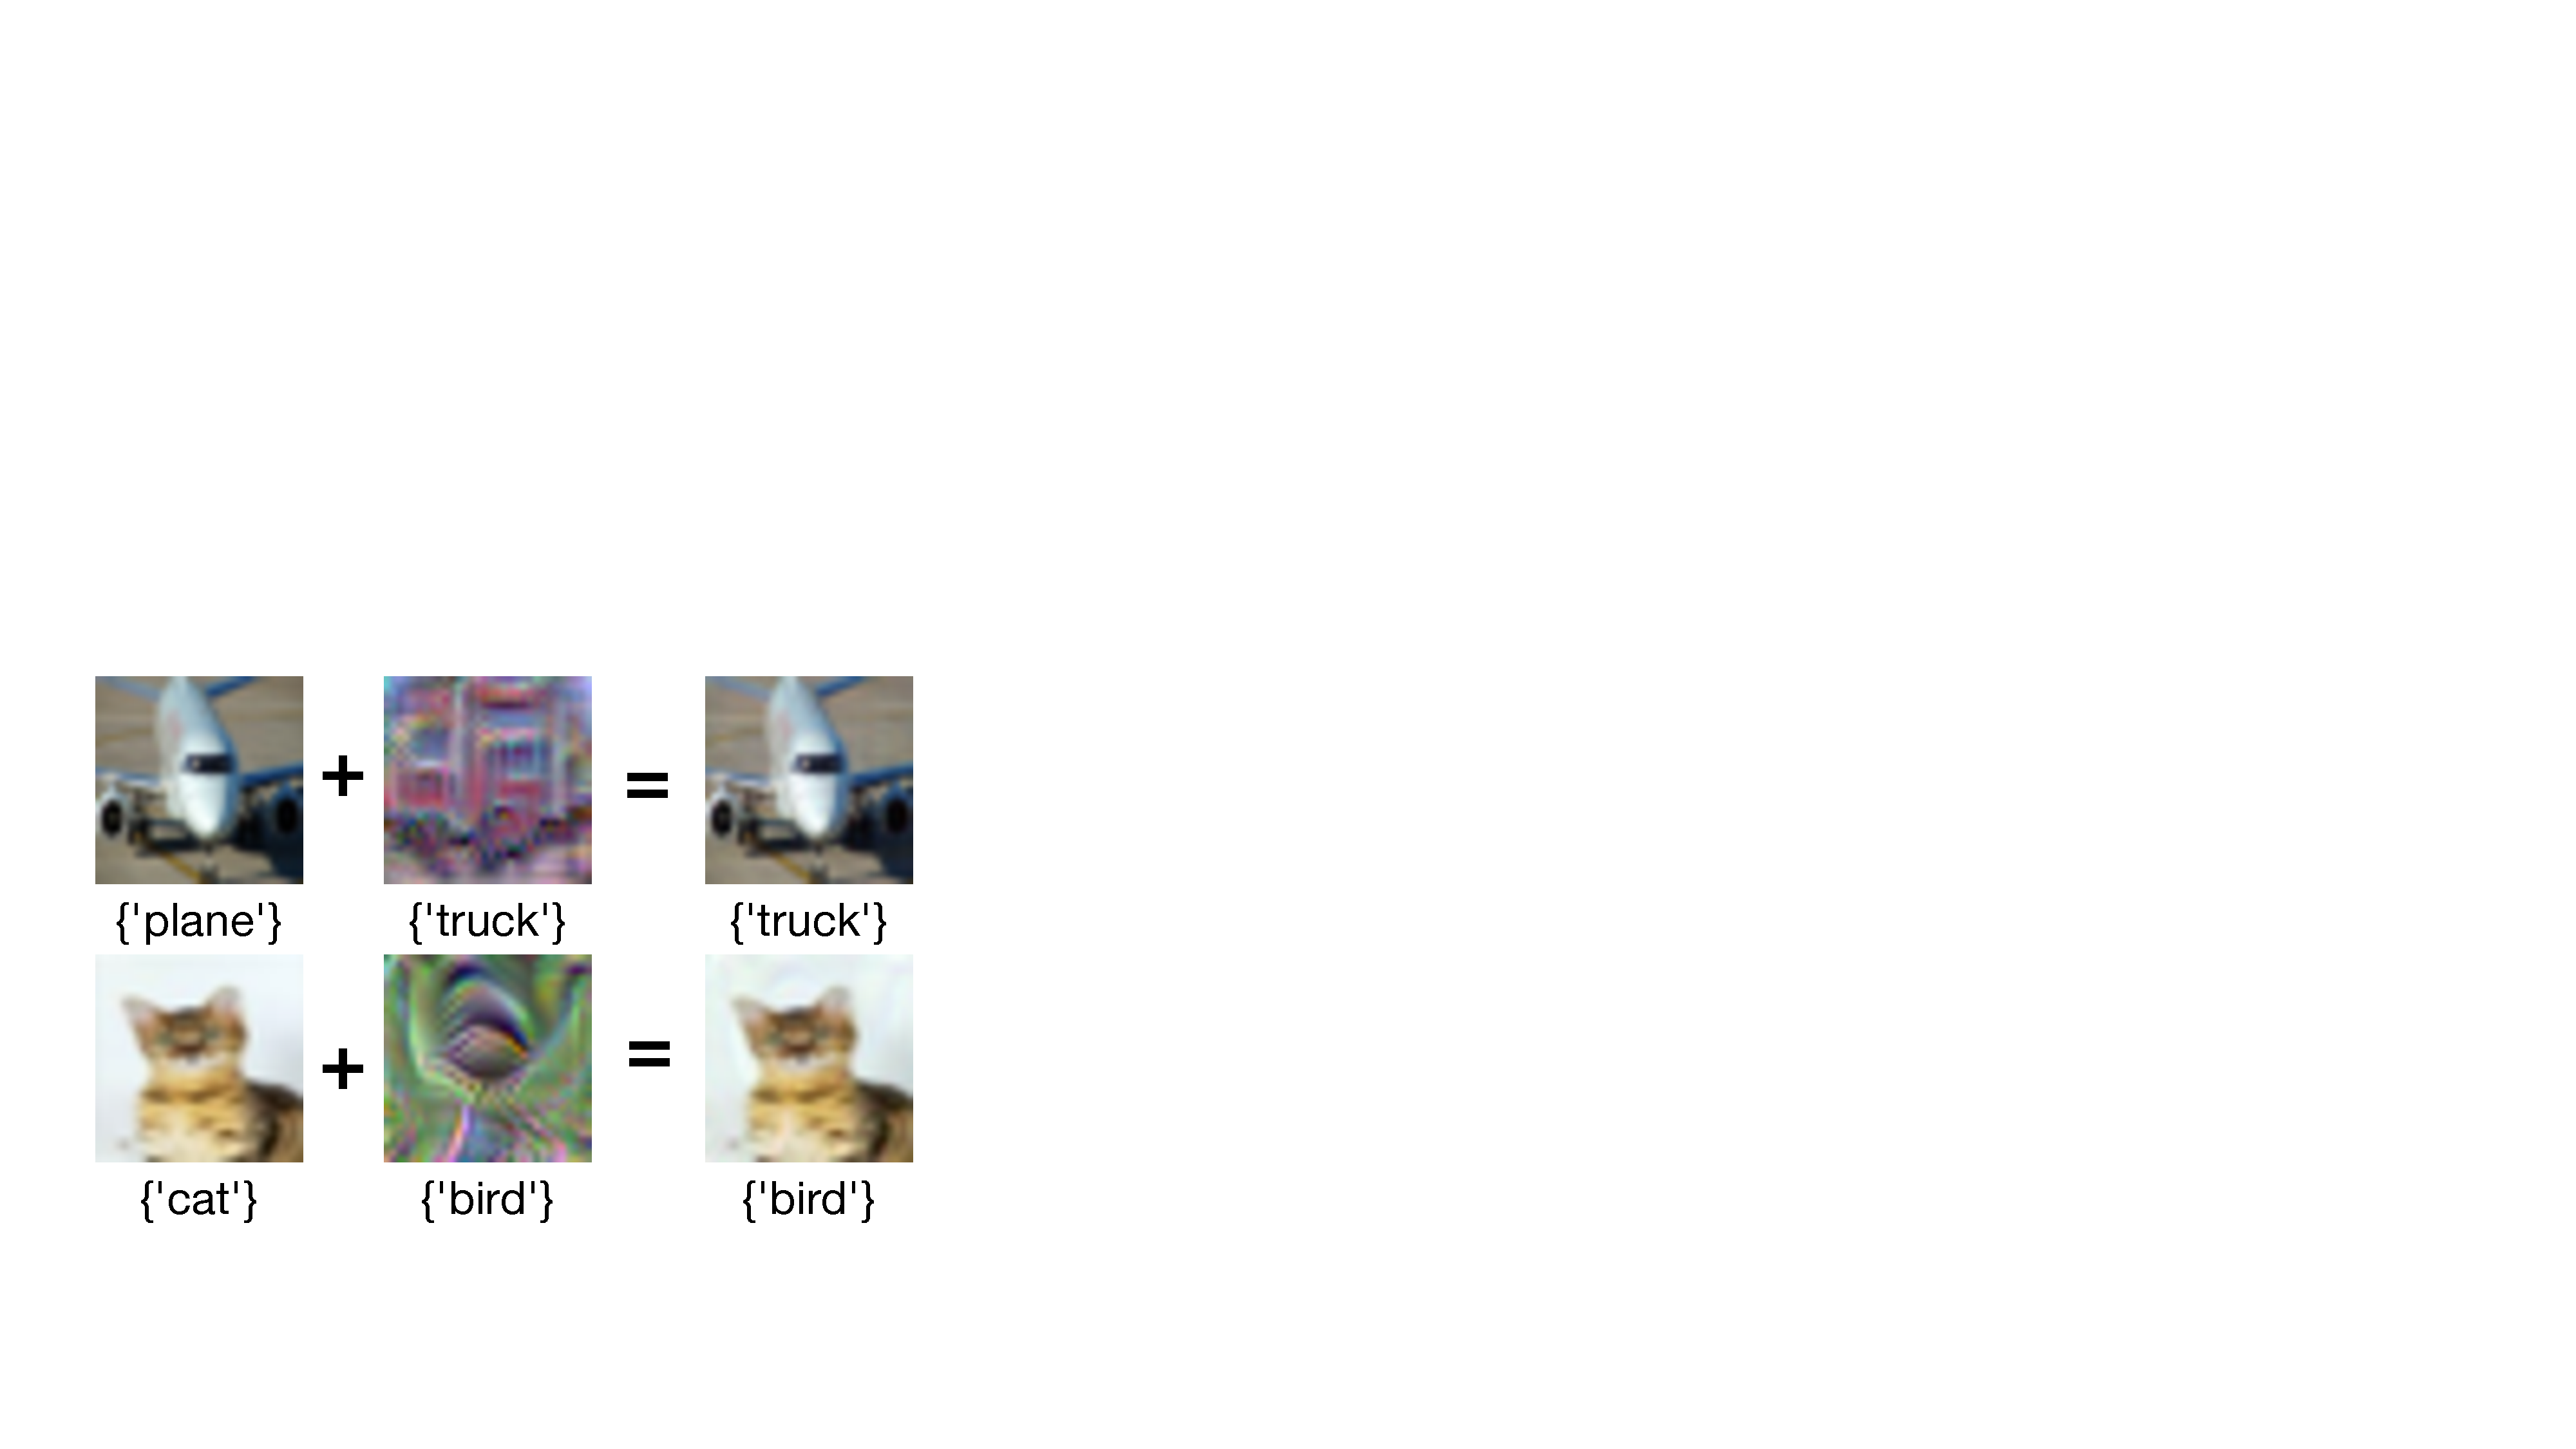
\includegraphics[width=0.8\linewidth]{./figure/adversarial.pdf}
%    \caption{Classification result of a mixed image of an original image and a DSV: The model's prediction follows that of the DSV even though the effect of the DSV is unnoticeable.}
   % \caption{ \hh{Classification result of mixed image of a original dog picture and a deer labeled DSV. Even though the DSV was combined with only 1$\%$ of the norm of the original image, the classification result was a deer. This indicates that the DSVs contain rich semantic information and can be easily used in global adversarial attacks.}}
%    \label{fig:adversarial}
% \end{figure}

% \jh{1. augmentation details. 2. model train details. 3. Datasets (SVHN, cifar10), 4. manifold hypothethis (SR 기법을 활용하였다) 5. hyperaparameters detilas 6. Outlier technique}

% \jh{2. DSVs reconstruction details, different augementation for fiarneess, flip, crop, translation, cutout. To maintain manifold hypothethis, we adopted SR technique, that is, generate DSVs for smaller maniofld. For Transfer learning analysis, we adopted Street View House Numbers (SVHN) dataset, which has same dimension for cifar10 dataset, and considered to be 'harder' dataset compared to mnist and coloredmnist dataset. We did transfer learning for classfier (at the very end fc layer), contrast to base model training, its training accuracy reached about 80\% accuracy, which does not satisfy primal condition. 
% \jh{For $L_\text{stationarity}$, we used learning rate $1e-3$ for non-augmentated DSVs, and we used learning for $5e-3$. $L_\text{Primal}$, we adopted $0.1$ and $1$ vice versa. It is due the diffence scale. Actual computed loss is 10 times higher for stationarity loss. To meet manifold condition when reconstructing DSVs, we adopted techinequies in Diffusion model, which is, synthethize data in low resolution, then upscale it to higher resolution. We downscaled image two times first and upscaled and continued optimization}

% \jh{For training pre-trained model $\Phi$, we adopted ConvNet architecture, which most common architecture is deep learning. A sequential convolutional layer followed by maxpool, and single-fully-connected layer for classification. Learning rate for $1e-3$ and weight decay for $5e-3$ in Adam optimizer. Also, we adopted flip, and crop, and the setting is different for DSVs reconstruction for fair comparison. When pretraining $\Phi$ for Street View House Numbers (SVHN), which is digit dataset and has same shape to cifar10, we only trained fully-connected layer from cifar10 pre-tained convnet that we pretrained just before. In that case, training accuracy scored 80\% .}
% \jh{3. Datasets, for ta}


% \jh{현재 추가할 figure - MNIST scratch, SVHN transfer. or vice versa. table의 경우 각 class별 model의 accuracy. lambda값과 accuracy의 상관관계, low rank의 confidence vs high rank의 confidence. Distillation 실험 표. Fairness Ai, ai}


% This was due to the differing scales. The actual computed loss for stationarity was ten times higher than for primal loss. To satisfy the manifold condition in reconstructing DSVs, we implemented techniques from the \nj{diffusion model}~\cite{diffusion:latent1}. This involved synthesizing data at a low resolution, then upscaling it to a higher resolution. We initially downscaled the image twice, then upscaled it, continuing with optimization. To reduce the impact of outliers, we choose the $L_1$ metric and apply the square root to \hh{the gradient term} when measuring distance.

% \nj{To obtain the pretrained weight $\theta^*$,} we chose the ConvNet architecture~\cite{convnet}, a common choice in deep learning. This architecture includes sequential convolutional layers followed by max pooling, and a single fully-connected layer for classification. The learning rate was set to \nj{\(10^{-3}\)} with a weight decay of \nj{\(0.005\)} using the Adam optimizer. Additionally, we employed flipping and cropping techniques, with settings differing from those used for DSVs reconstruction to ensure fair comparison. For pretraining \(\Phi\) on the Street View House Numbers (SVHN) dataset~\cite{dataset:svhn}, a digit dataset with dimensions similar to CIFAR-10~\cite{dataset:cifar10}, we exclusively trained the fully-connected layer of the CIFAR-10 pre-trained ConvNet. This approach resulted in a training accuracy of 80\%. \jh{When retraining the model with DSVs, we used large learning rate of 0.1 and a $\rho$ value of 0.0001 were utilized for the SAM optimizer to adhere to the principle of margin maximization~\cite{largelr, samopt}.}
% \jh{For DSVs synthesis, we used a single 1080TI GPU and it took 15 minutes.}




% 위 Sec.~\ref{sec:DKKTcondition}에서도 설명했듯이 primal feasibility 조건은 모델이 DSV들을 정확한 class로 분류하게 하는 역할을 하며 (correctly discriminate its support vectors), stationary condition은 DSV들이 decision boundary 쪽으로 가게하는 역할을 한다. Fig.~\ref{fig:primalstat}를 보면 cat과 deer에 대해서 각각 primal과 stationary condition만을 사용하여 DSV들을 뽑은 결과를 나타낸다. 이때 primal condition만 사용하였을 때는 classify하기 위한 texture과 같은 global한 특징들 잡은 반면에 stationary condition만 사용하였을때는 실제 데이터셋과 유사한 shape과 edge 특징들을 잡음을 알 수 있다. Stationary condition에서는 class constraint가 직접적으로 반영되지 않기때문에 dataset과 유사한 artifacts 들은 만들어내지만, class specific하게 보정하지 못하기 때문에 실제로 
%  해당 샘플들에 대하여 model accuracy가 많이 떨어진다.따라서 classify 역할을 하는 primal condition이 DSV 추출과정에서는 classifier guidence역할을 한다는 사실을 알 수 있다. 나아가서 일반적인 generative 모델들이 classifier guidence를 쓰듯이 필요에 따라서 두 loss 간의 적절한 interpolation을 통하여 classfier guidence를 조절하여 generative model들 처럼 sampling을 할 수 있다. 


% \begin{table}[]
% \tiny
% \centering
% \caption{현재 25\%까지 나오는데 더 해보겠습니다. TODO: Coreset selection 부분들도 넣어보기: 14.4 $\pm$ 2.0 (Random), Herding (21.2 $\pm$ 1.2), Forgetting (13.3 $\pm$ 1.2)}
% \label{table:datasetedistillation33}
% \begin{tabular}{c|c|c|c|c|c}
%          & Img/cls & ratio & DD & DC & DSV (ours) \\ \cline{4-6} 
%          &         &       & Random & Herding & Forgetting \\ \hline
% CIFAR-10 & 1       & 0.02  & 27.3\% & 28.3\% & 25.x\% \\
% \end{tabular}
% \end{table}

% \begin{table}[]
% \tiny
% \centering
% \caption{현재 25\% 까지 나오는데 더 해보겠습니다, TODO: Coreset selection 부분들도 넣어보기 14.4 $\pm$ 2.0 (Random), Herding (21.2 $\pm$ 1.2), Forgetting 13.3 $\pm$ 1.2}
% \label{table:datasetedistillation}
% \begin{tabular}{c|cc|cccc}
%          & Img/cls & ratio & DD & DC & DSV (ours) & Full Dataset \\ \hline
% CIFAR-10 & 1       & 0.02  &  27.3 \%  &  28.3\%  &         25.x\%    & 84.09          
% \end{tabular}
% \end{table}


% [1]Deep Total Variation Support Vector Networks, 10.1109/ICCVW.2019.00365
% [2]When Ensemble Learning Meets Deep Learning: a New Deep Support Vector Machine for Classification, 10.1016/j.knosys.2016.05.055 [3]An Ensemble of Deep Support Vector Machines for Image Categorization, 10.1109/SoCPaR.2009.67
% [4]Deep Support Vector Classification and Regression, 10.1007/978-3-030-19651-6_4
% [5]A Complete Deep Support Vector Data Description for One Class Learning, 10.1109/ACCESS.2023.3325734
% [6]Deep support vector machine for hyperspectral image classification, 10.1016/j.patcog.2020.107298
% [7]Contrastive deep support vector data description, 10.1016/j.patcog.2023.109820
% [8]Deep neural mapping support vector machines, 10.1016/j.neunet.2017.05.010 % [9]Deep Learning using Linear Support Vector Machines, https://doi.org/10.48550/arXiv.1306.0239 (https://doi.org/10.48550/arXiv.1306.0239) [10]Totally Deep Support Vector Machines, https://doi.org/10.48550/arXiv.1912.05864 (https://doi.org/10.48550/arXiv.1912.05864)


\subsection{\gm{DSVs: Revival of Support Vectors in Deep Learning}}
\begin{wrapfigure}{t}{5.2cm}
% \begin{figure}[t]
  \centering
   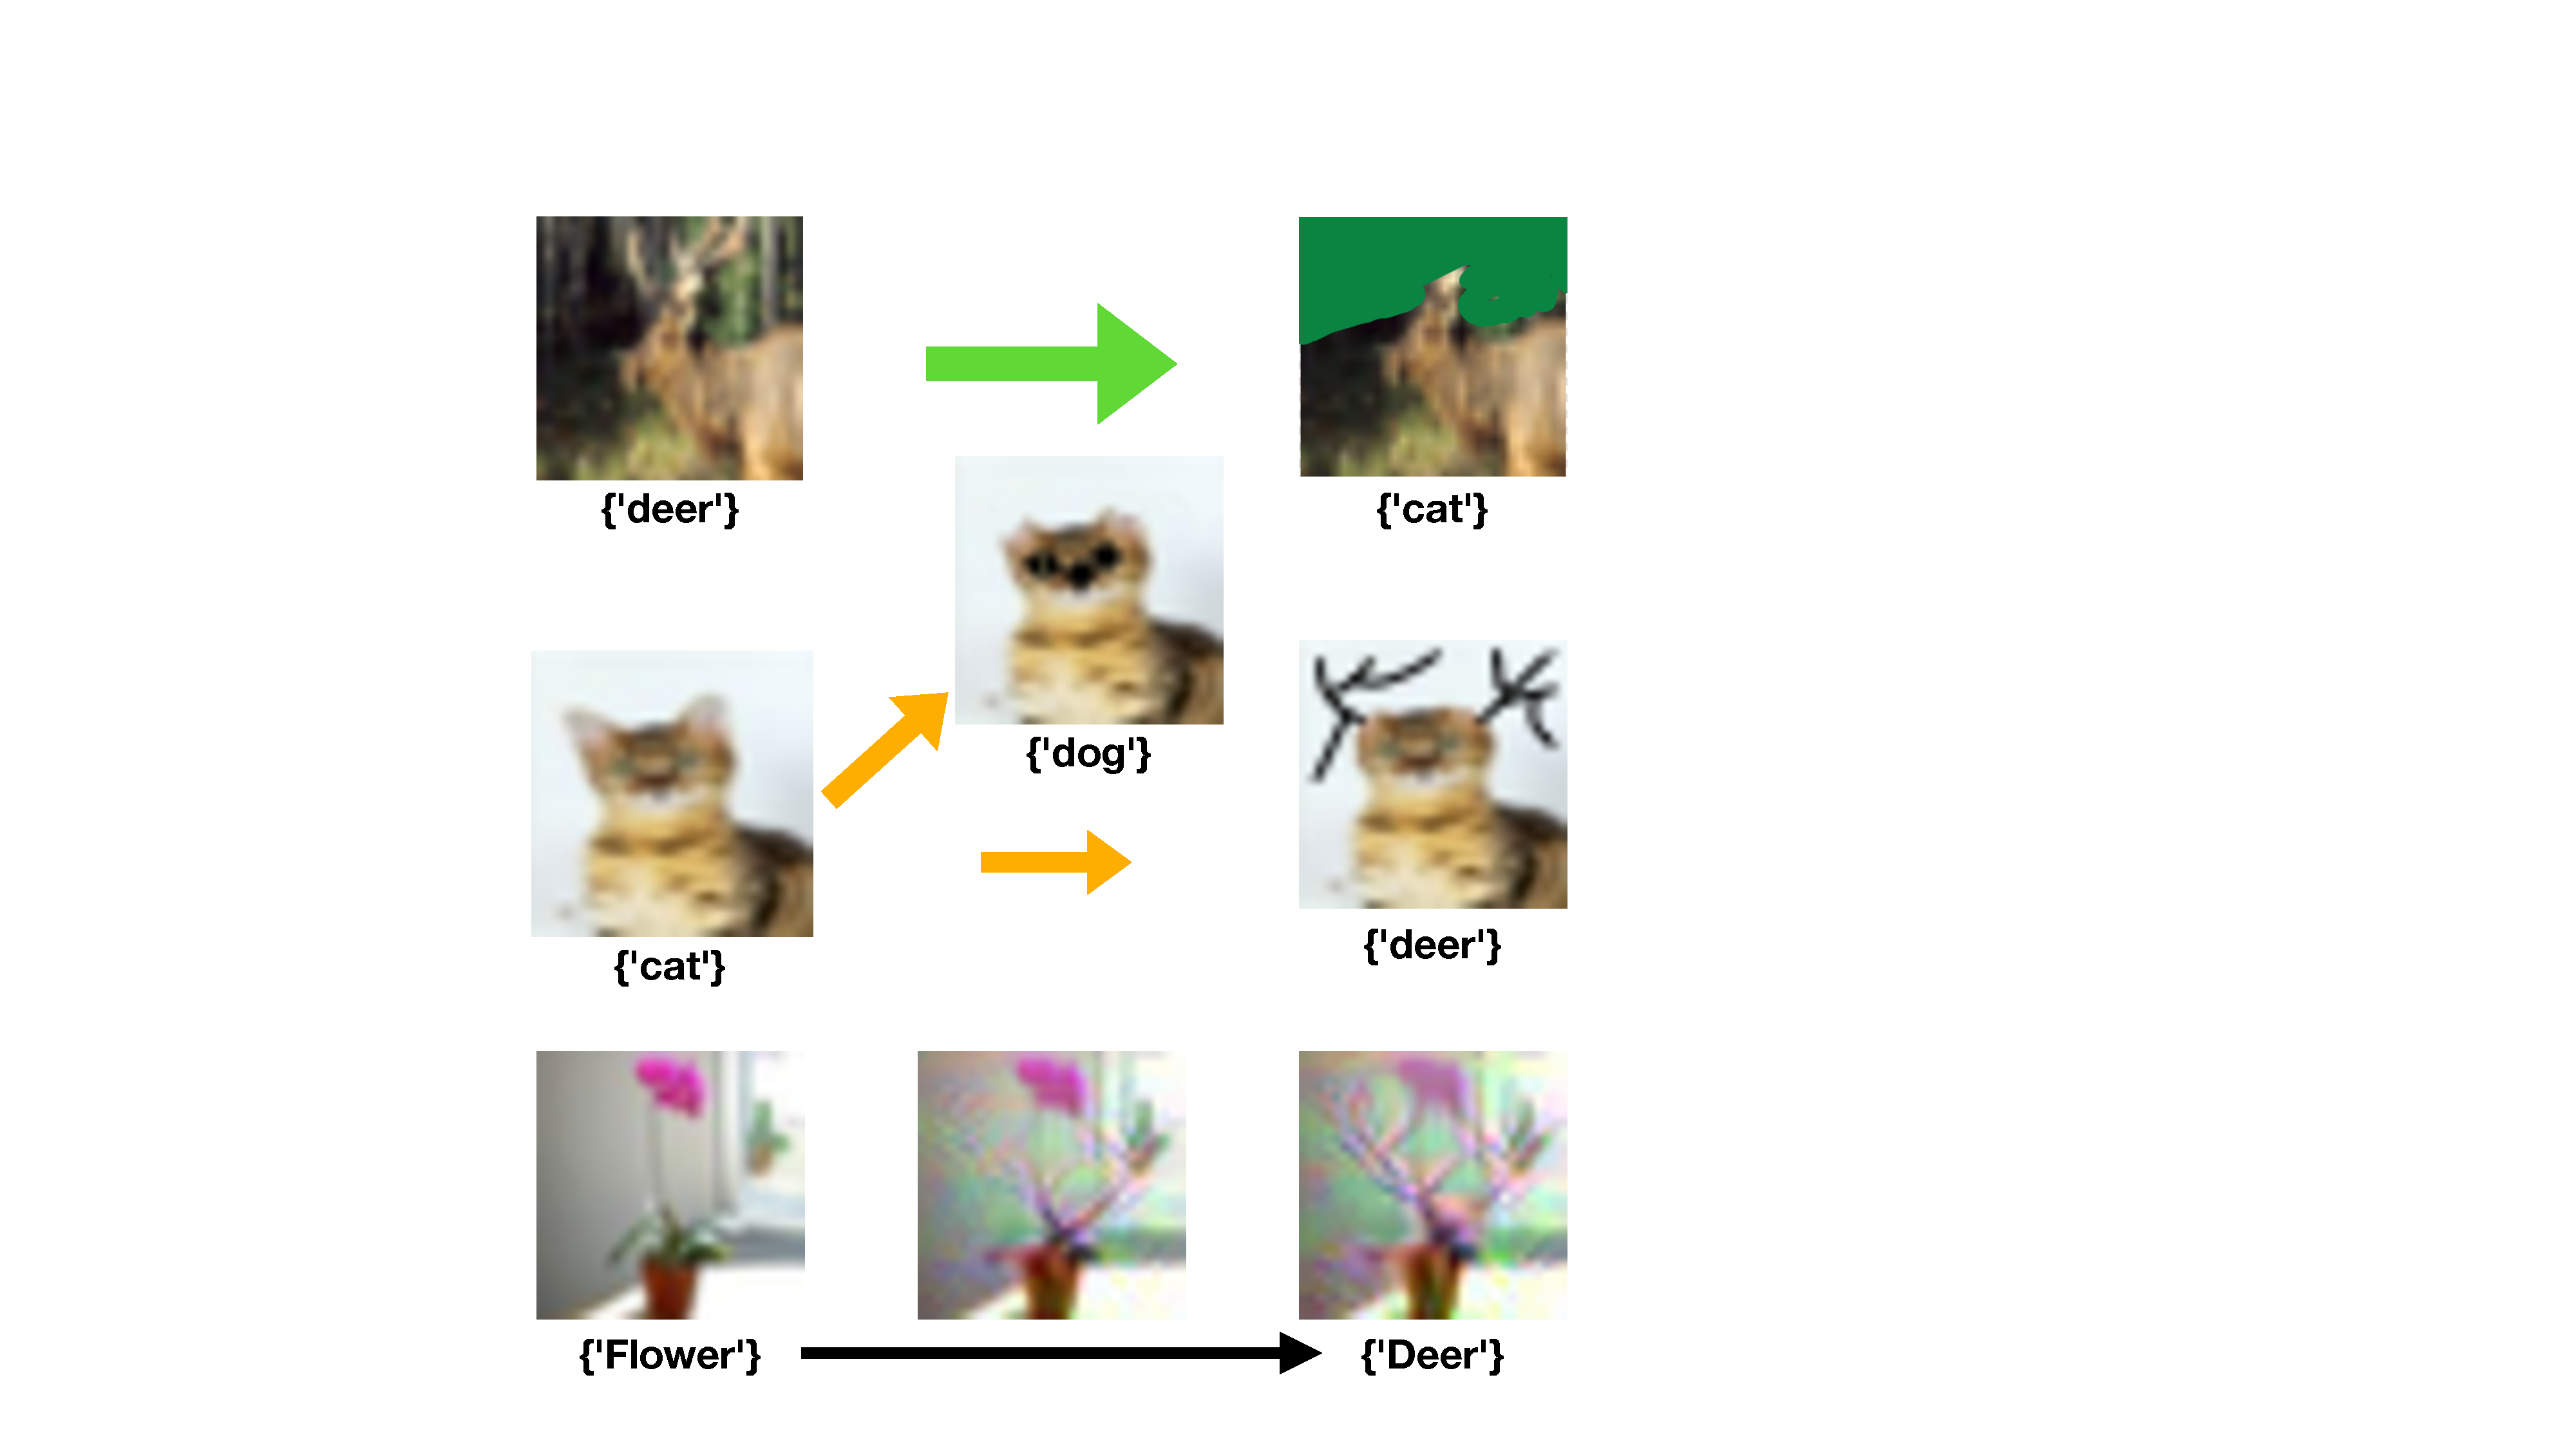
\includegraphics[width=5cm]{./figure/editimages.pdf}
   \caption{\jh{Model predictions for original versus DSV-informed edited images. (Top) Images were altered manually \nj{based on} decision criteria derived from DSVs, influencing \nj{the model's prediction. (Bottom) Images were altered based on DeepKKT loss.}} %to reclassify them.
   }
   % \caption{\hh{ Depiction of model confidence scores for both masked and non-masked image of a deer in the CIFAR-10 training dataset. In Fig.~\ref{fig:DSVSET}, a DSV deer emphasizes antler characteristics, while a DSV cat underscores sharp ear features. When the antlers are masked to resemble sharp ears, the model infers the image as a cat with 89.5$\%$ confidence, while the confidence for it being a deer drops to 5.3$\%$.}}
   \label{fig:Painting}
% \end{figure}
\end{wrapfigure}
%Decoding Black-Box in Deep Learning}
% \paragraph{DSVs Implicitly Meet Complementary Slackness}\label{sec:slackness}
% DSV는 complementary slackness를 안넣었는데도 empirical하게 된다

% As we stated in Sec.~\ref{sec:KKTcondition}, complementary slackness mandates support vectors lie in decision boundary and we did not include for the sake of computation cost and ambiguity. However Fig.~\ref{fig:lambda_entropy} suggests that even if the case, DSVs implicitly suffices the condition. For selection process, DSVs with high lambda is lower than small lambda DSVs (This is because we assigned lambda randomly). However, as train progresses, we can see the selected highest-top-5 lambda samples (이 부분 wording 별로, lambda중 top 이란 말,,)'s entropy increases while lowest-top-50 lambda samples (i.e., where images are not distinguished as support vector, lambda = 0) entropy decreases. This mean the selected sets are more uncertain, which implies it is located near boundary.

\paragraph{DSVs meet SVM characteristics}\label{sec:slackness}

\jh{As discussed in Section~\ref{sec:KKTcondition}, the principle of complementary slackness within the KKT conditions suggests that support vectors should be situated on the decision boundary, implying that support vectors typically exhibit high uncertainty from a probabilistic perspective, \ie they possess high entropy. While DeepKKT does not explicitly incorporate the \nj{complementary} slackness condition due to computational costs and ambiguity, \nj{Fig.~\ref{fig:lambda_entropy} suggests} that DSVs implicitly fulfill this condition; During the training process, we observe an increase in the entropy of DSV candidates, \nj{hinting that the generated DSVs are close to the decision boundary}.}

% Moreover, in \nj{an} SVM, the Lagrangian multiplier, $\alpha$, acts as a natural measure to determine which support vector is more important than others.
% \jh{Similarly, we can perform a comparable role using DeepKKT condition. \jh{Using the condition, we trained Lagrangian multiplier $\lambda$, which is assigned to each image.} Fig.~\ref{fig:correlation} \nj{shows} a strong correlation between the sum of $\lambda$ values for each class and \nj{its} test accuracy. This finding is intriguing because, despite the model achieving nearly 100\% accuracy during training due to overparameterization, DSVs provide insights into categorical generalization in the test phase.} \jh{Not only measuring its credibility, as large $\lambda$ refers `important' image for training images, $\lambda$ could serve as natural core-set selection measure. Table.\ref{table:coreset} shows this is actually true. On CIFAR10\cite{dataset:cifar10} dataset, we selected images with high-lambda values, and retrained with selected images, in this case, the performance scored higher compared to random selection. This characteristic resembles support vectors, as we can reconstruct the model with support vectors.}

%\begin{wrapfigure}{l}{7cm}
%\vspace{-2mm}
%\begin{figure}[t]


% \begin{figure}[t]  
%   \begin{minipage}[b]{.6\linewidth}
%   \centering
%     \begin{subfigure}[b]{0.48\linewidth}
%     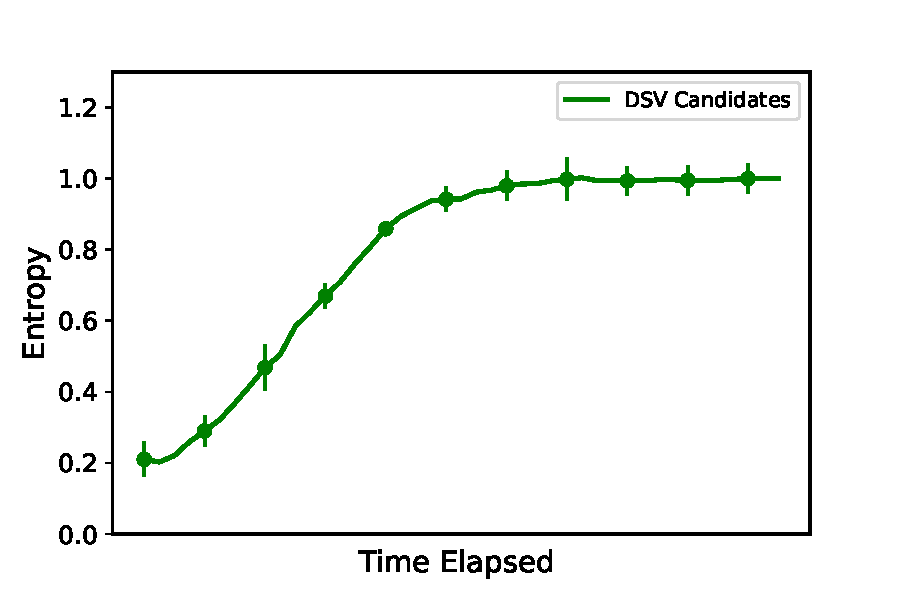
\includegraphics[width=\linewidth]{./figure/Entropy_DSV.pdf}
%     \caption{\nj{Entropy change of DSV candidates over time}}
%     \label{fig:lambda_entropy}
%   \end{subfigure}
%   \hfill
%   \begin{subfigure}[b]{0.48\linewidth}
%     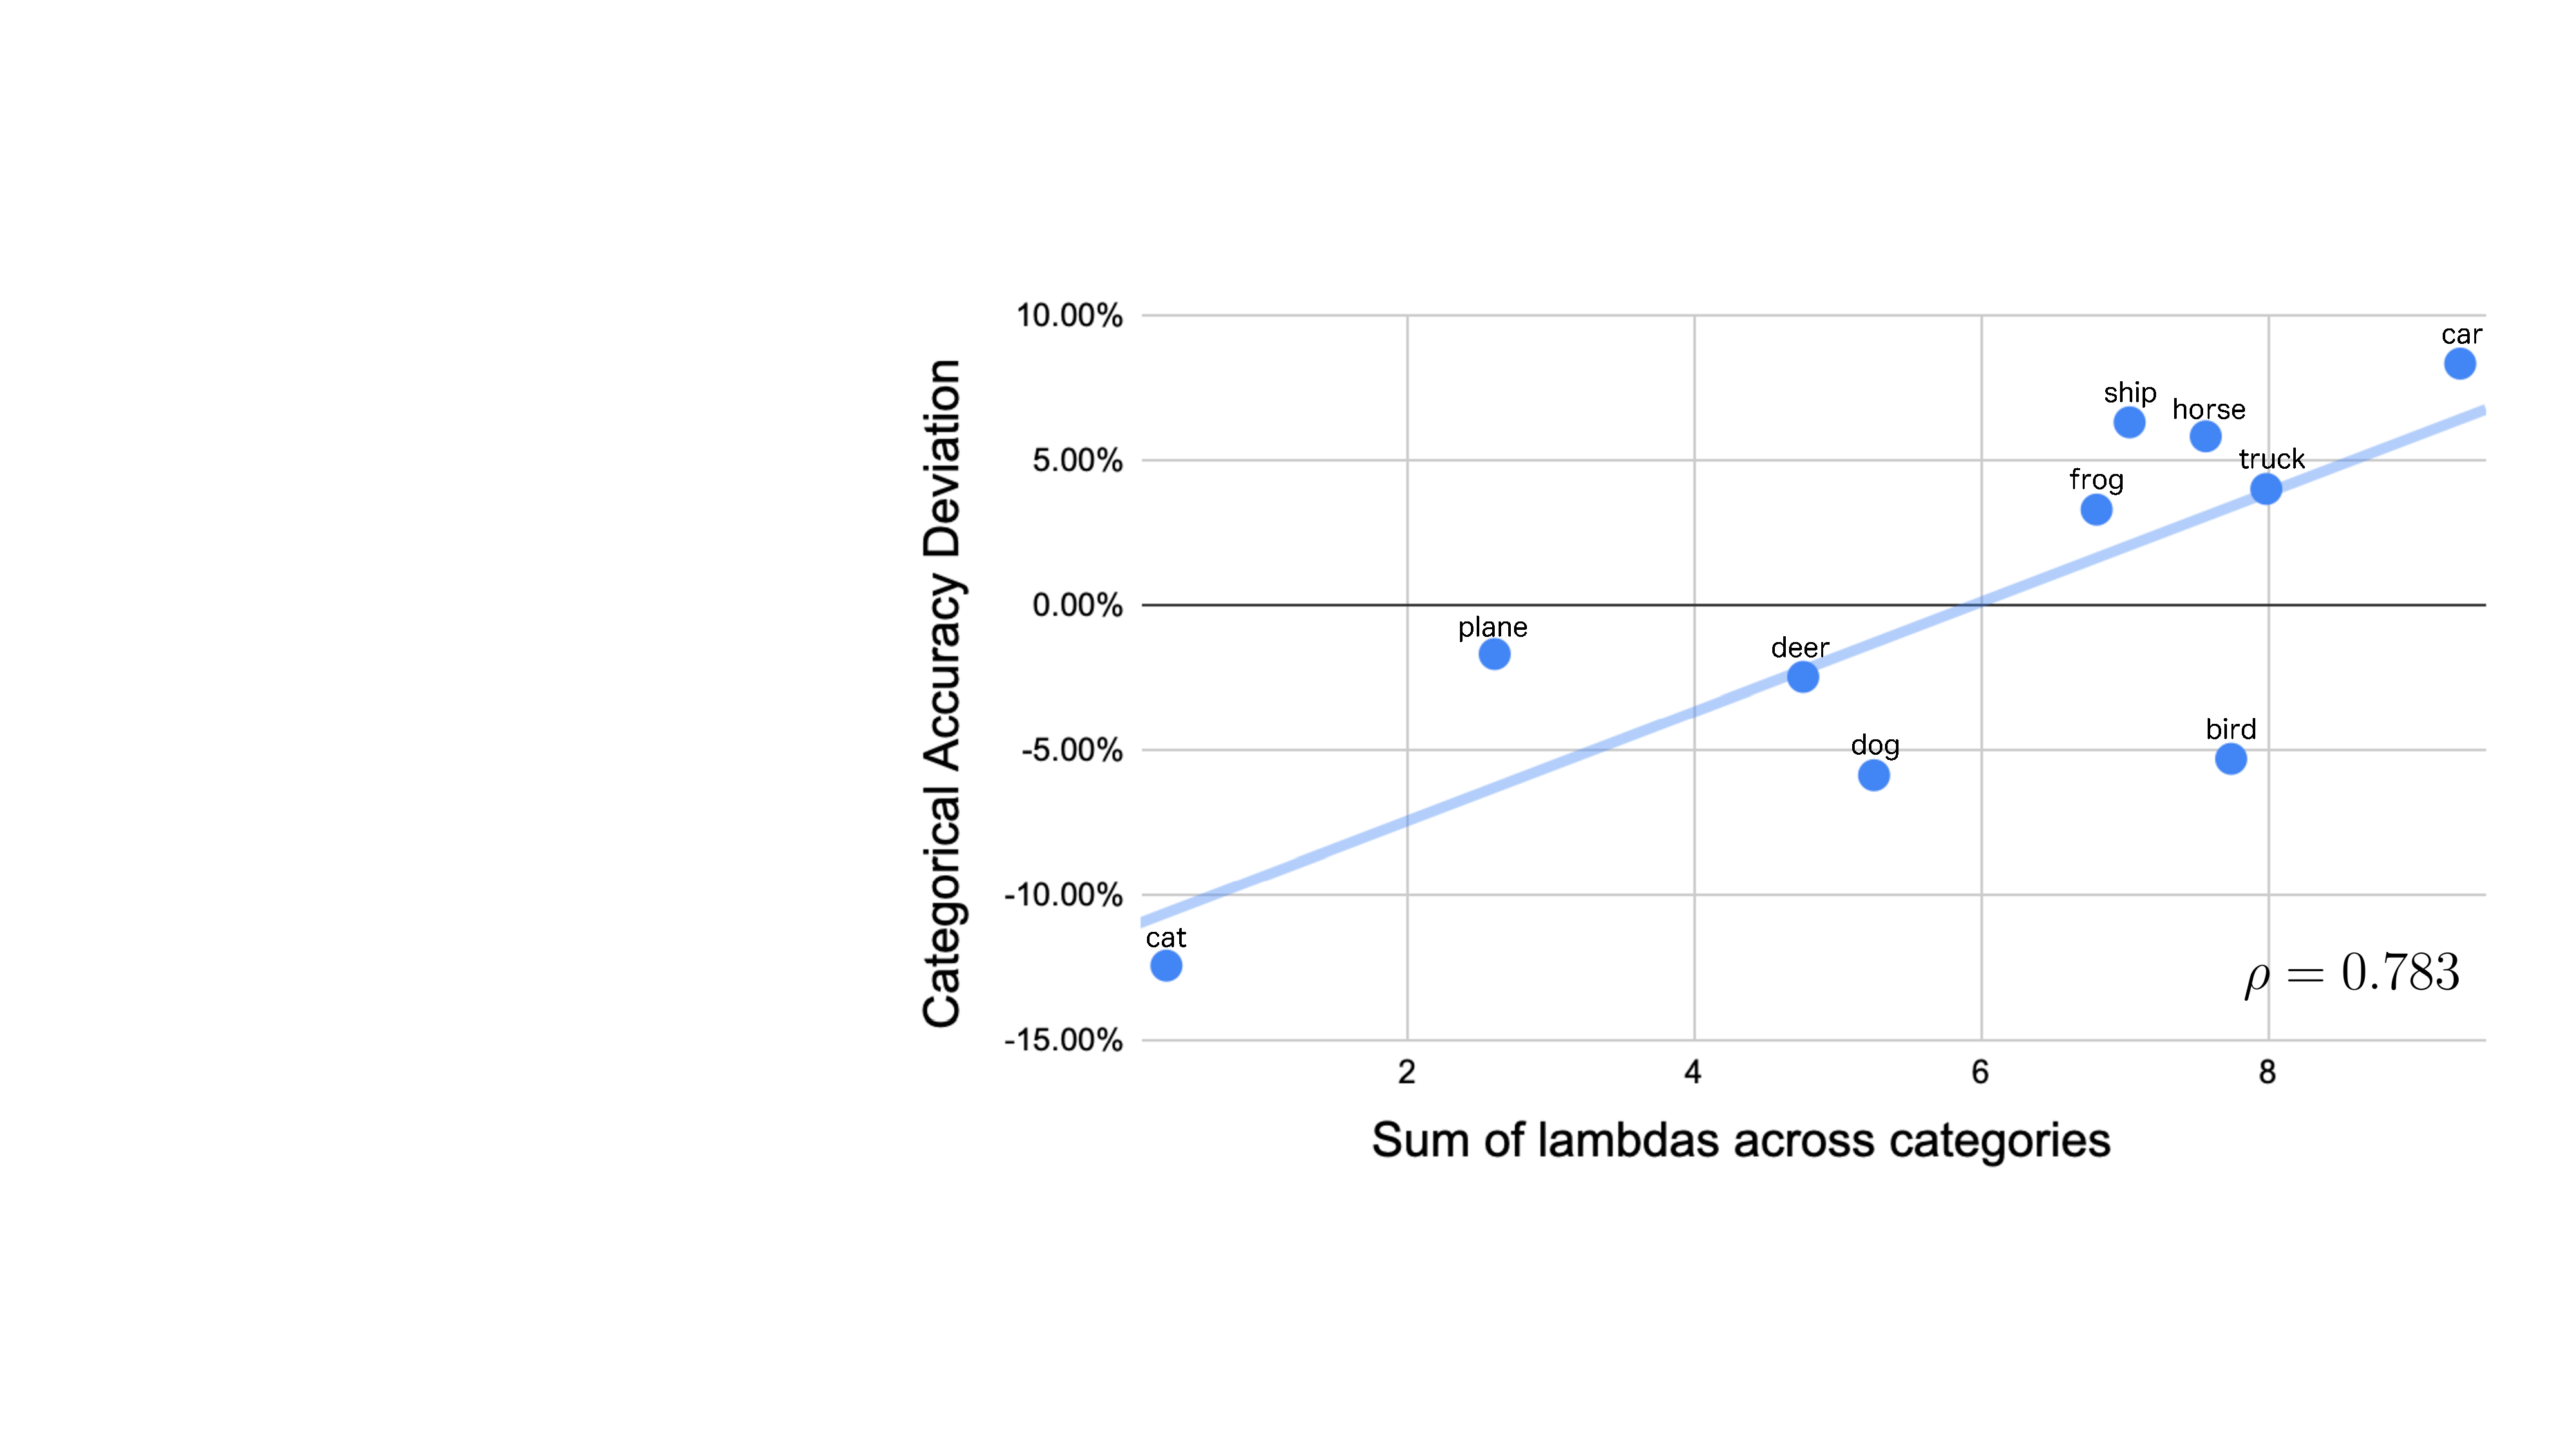
\includegraphics[width=\linewidth]{./figure/pearson.pdf}
%     \caption{Correlation between classwise mean test accuracy and \nj{the} sum of $\lambda$'s}
%     \label{fig:correlation}
%   \end{subfigure}
%   \setcounter{figure}{1}
%   \captionof{figure}{\nj{Characteristics of DSVs}%\gm{figure2여야 하는데, figure 3으로 되어있습니다}
%   }
%   \end{minipage}  
% \hfill 
% \begin{minipage}[b]{.35\linewidth}
% \vspace{-10mm}
% \centering
% \resizebox{\linewidth}{!}{
% \begin{tabular}{l|l|rr}
% \hline
% img/cls & ratio (\%) & \multicolumn{1}{l}{Random} & \multicolumn{1}{l}{selected DSVs } \\ \hline
% 50      & 1          & 46.16 $\pm$ 1.93           & 48.91 $\pm$ 0.90               \\
% 10      & 0.2        & 30.08 $\pm$ 1.96           & 33.69 $\pm$ 2.05               \\
% 1       & 0.02       & 14.26 $\pm$ 0.99           & 16.83 $\pm$ 0.29               \\ \hline
% \end{tabular}
% }
% \vspace{5mm}
% \captionof{table}{\jh{In coreset selection benchmarks \nj{using the CIFAR-10 dataset, the DeepKKT condition is used as the selection criterion. Images with the highest $\lambda$ for each class were chosen to train a network. }}}
% \label{table:coreset}
% %\end{wraptable}
% \end{minipage}
% \vspace{-5mm}
% \end{figure}

\jh{\nj{In addition, we can infer the importance of a sample in the decision process by utilizing the DeepKKT condition. We} trained the Lagrangian multiplier $\lambda$ \nj{for} each \nj{test} image. Figure~\ref{fig:correlation} shows a strong correlation between the sum of $\lambda$ values for each class and its test accuracy. This finding is intriguing because, despite the model achieving nearly 100\% accuracy during training due to overparameterization, DSVs provide insights into categorical generalization in the test phase. Not only does measuring its credibility indicate that a large $\lambda$ refers to an `important' image for training, but $\lambda$ could also serve as a natural core-set selection measure. Table~\ref{table:coreset} shows this to be true. On the CIFAR-10~\cite{dataset:cifar10} dataset, we selected images with high $\lambda$ values and retrained \nj{the network} with the selected images. In this case, the \nj{selected DSVs show higher test acccuracies} compared to random selection. This characteristic resembles \nj{that of} support vectors, as \nj{the model can be reconstructed} with support vectors.}



Finally, Fig.~\ref{fig:generated} demonstrates the high fidelity of the generated DSVs, providing practical evidence that these DSVs lie on the data manifold.
Similar to how support vectors are reconstructed in \nj{an} SVM, the DeepKKT condition \nj{enables} the reconstruction of these vectors without \nj{referencing} training data. This \nj{shows} the effectiveness and adaptability of \nj{our DeepKKT} in capturing key data features.
%Similar to the way support vectors are reconstructed in SVM, the DeepKKT condition facilitates the reconstruction of these vectors without relying on training data. This capability underscores the effectiveness and adaptability of the DeepKKT approach in reflecting key data features.}

% As discussed in Sec.~\ref{sec:KKTcondition}, the principle of complementary slackness within the KKT conditions suggests that support vectors should be situated on the decision boundary. \jh{Meaning, support vector should have large uncertainty in probabilistic perspective \ie has high entropy}. As DeepKKT does not explicitly incorporated slackness condition due to computational costs and ambiguity, Fig.~\ref{fig:lambda_entropy}, it appears that DSVs implicitly fulfill this condition. Notably, during the training process, we observe an increase in the entropy of DSV candidates.

% \jh{Also, in SVM, the Lagrangian multiplier $\alpha$, acts as a natural measure to determine which support vector is more important than others. Similarly, DSVs can \nj{act} a comparable role. Fig.~\ref{fig:correlation} indicates a strong correlation between the sum of \nj{$\lambda$'s per each class and  actual classwise}  test accuracy. This phenomenon is intriguing because, despite the model achieving nearly 100\% accuracy during training due to overparameterization, DSVs can provide insights into the categorical generalization in the test phase.}

% \jh{Finally, Fig.\ref{fig:my_label} shows that generated DSVs lie data manifold. As we can reconstruct support vectors from SVM, DeepKKT condition reconstructed support vectors without any training data.}

% \jh{Furthermore, support vector should act as im}

% \jh{From a probabilistic perspective, high entropy indicates greater uncertainty. This is a strong indicator that these samples are positioned near the decision boundary, as they are the ones for which the model is least certain about their classification. This aligns with the complementary slackness principle, which posits that support vectors play a crucial role in defining the decision boundary.}

% \paragraph{Predicting Model Dynamics With DSVs’ Inherent Importance}


% \jh{In SVM, the Lagrangian multiplier $\alpha$, acts as a natural measure to determine which support vector is more important than others. Similarly, DSVs can \nj{act} a comparable role. Fig.~\ref{fig:correlation} indicates a strong correlation between the sum of \nj{$\lambda$'s per each class and  actual classwise}  test accuracy. This phenomenon is intriguing because, despite the model achieving nearly 100\% accuracy during training due to overparameterization, DSVs can provide insights into the categorical generalization in the test phase.}










\paragraph{DSVs \nj{for} Few Shot Dataset Distillation}
\jh{DeepKKT emerges as a pioneering algorithm tailored for practical \nj{dataset distillation}. \nj{DSVs} addresses two critical concerns: 1) Protecting private information through data synthesis, and 2) Reducing the communication load by minimizing the size of \nj{data transmission}. Traditional distillation algorithms encounter a fundamental paradox; \nj{as} data predominantly originate from edge devices like smartphones \cite{FL1, fl_start, fl2}, \nj{the} requirement to access \nj{the} entire dataset introduces significant communication overhead and heightens privacy concerns.}

% Traditional algorithms often struggle with data sourced from edge devices like smartphones \cite{FL1,fl2}, as they typically require access to the entire dataset, usually centralized, leading to significant communication overhead and heightened privacy risks. This challenge underscores the need for a few-shot distillation setting, where only a single trained model and a small fragment of data from a larger dataset are utilized. The DeepKKT condition is particularly suited for addressing this issue.



%
%
% \jh{이 부분의 위치 정해야함} \hh{6.1에 들어가면 될것같음}


% \begin{wrapfigure}{t}{5.2cm}
% % \begin{figure}[t]
% \vspace{-5mm}
%   \centering
%    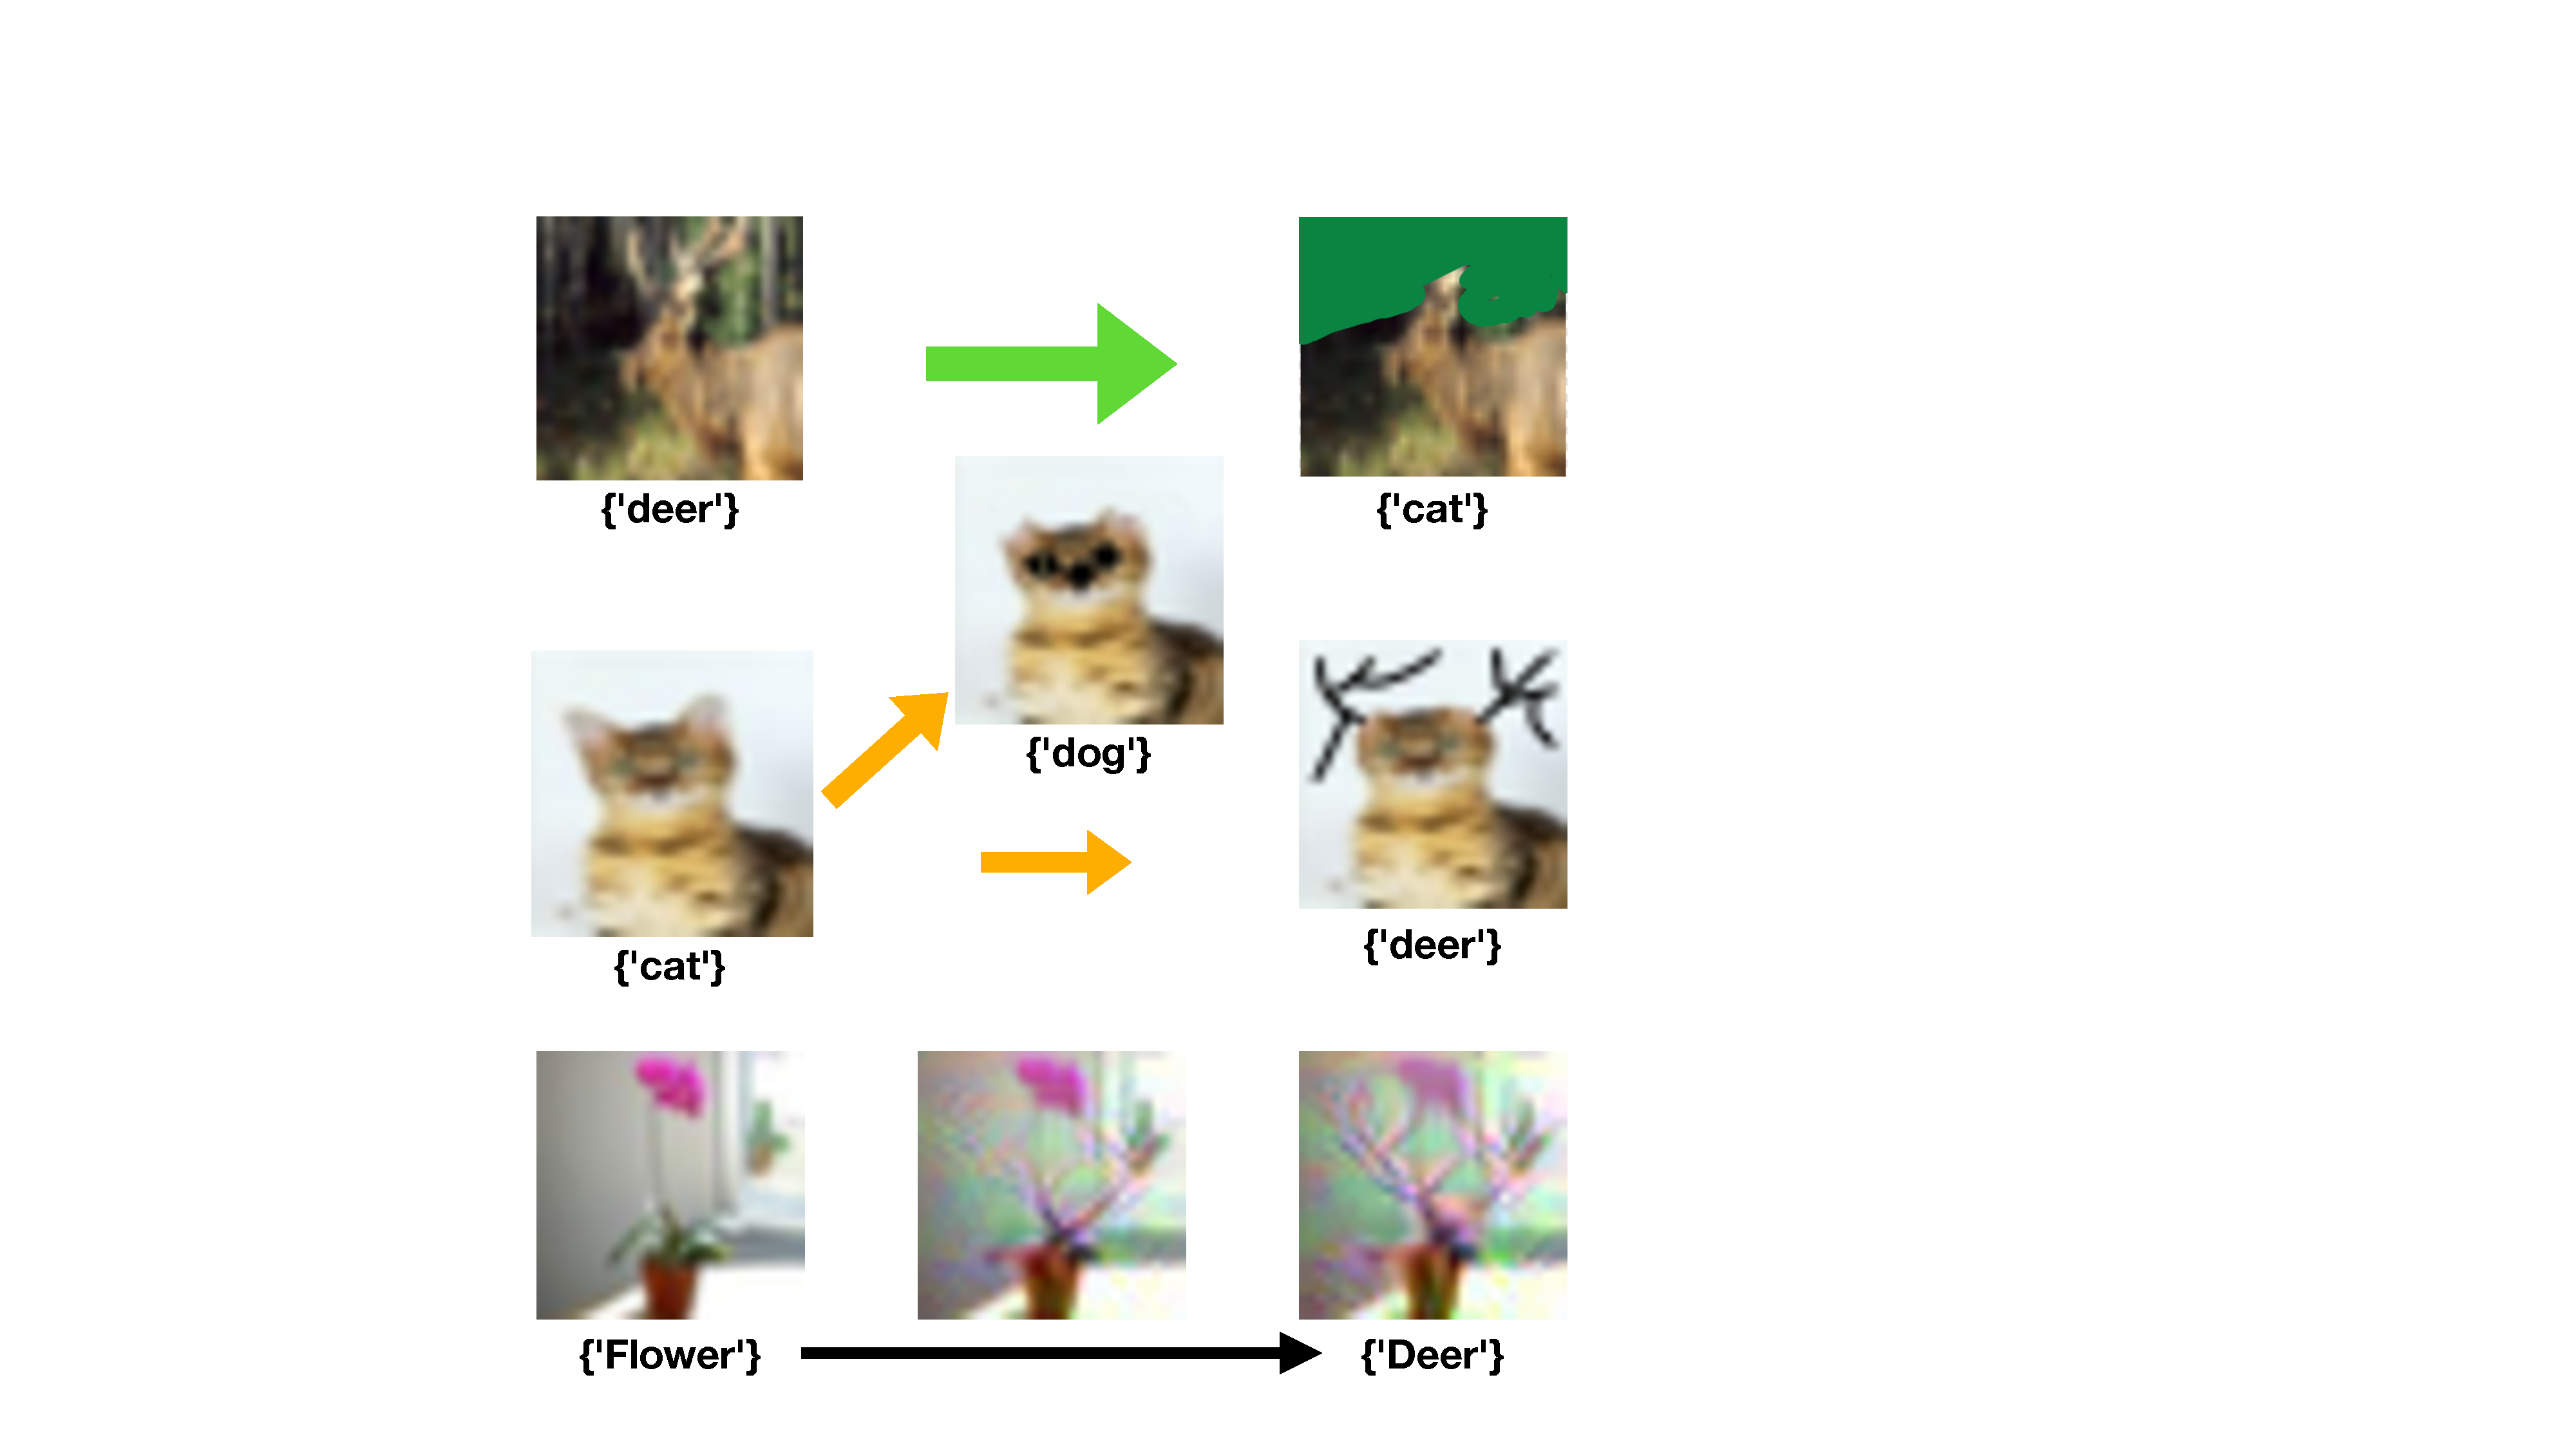
\includegraphics[width=5cm]{./figure/editimages.pdf}
%    \caption{\jh{Model predictions for original versus DSV-informed edited images. (Top) Images were altered manually \nj{based on} decision criteria derived from DSVs, influencing \nj{the model's prediction. (Bottom) Images were altered based on DeepKKT loss.}} %to reclassify them.
%    }
%    % \caption{\hh{ Depiction of model confidence scores for both masked and non-masked image of a deer in the CIFAR-10 training dataset. In Fig.~\ref{fig:DSVSET}, a DSV deer emphasizes antler characteristics, while a DSV cat underscores sharp ear features. When the antlers are masked to resemble sharp ears, the model infers the image as a cat with 89.5$\%$ confidence, while the confidence for it being a deer drops to 5.3$\%$.}}
%    \label{fig:Painting}
%    \vspace{-5mm} 
% % \end{figure}
% \end{wrapfigure}
%
%

\nj{Our DeepKKT relies solely on a pre-trained model without relying on the training dataset}. This unique approach eliminates the need for edge devices to store or process large volumes of private data. 
%By \nj{iteratively updating the} initial point noise \nj{towards a realistic DSV image using DeepKKT constraints, it acts} as a powerful few-shot dataset distillation algorithm, as demonstrated in 
% Table~\ref{table:fewshot}. While traditional methods suffer significant performance drops under \nj{these scenarios} and furthermore, traditional methods cannot implement zero-shot scenarioes.
% \jh{DeepKKT maintains efficacy by requiring only minimal data, such as a single image per sample (\ie initialization with real data), or zero-image per sample. For zero-image setting, we initialized the image with other datasets for diversity.}
\jh{\nj{As shown in Table~\ref{table:fewshot}, while} traditional methods suffer significant performance drops under these scenarios \hh{and are incapable of implementing zero-shot scenarios. Conversely DeepKKT remains effective, requiring only minimal data: a single image per sample (\ie initialization with real data), or in some cases, no images at all.} For the zero-image setting, we initialized the images with data from other datasets to ensure diversity.}

%This minimal data requirement \nj{reduces the operational overhead and} enhances the algorithm's practicality in scenarios constrained by data availability or privacy concerns.


% In the context of dataset distillation, DeepKKT can be used as a pioneering algorithm tailored for practical scenarios. Dataset distillation primarily addresses two key issues: 1) Protecting private information through data synthesis, and 2) Reducing the communication load by minimizing the data size. Traditional algorithms, however, face a paradox, particularly when data originates predominantly from edge devices like smartphones \cite{FL1,fl2}. These algorithms typically require access to the entire dataset, presumably centralized, leading to significant communication overhead and privacy concerns. 
% %Moreover, we observed a substantial decline in performance with reduced training data volumes, as detailed in Section~\ref{sec:reliance}. 
% Contrasting with these approaches, DeepKKT operates independently of any dataset, relying solely on a pre-trained model. This approach eliminates the need for edge devices to store extensive private data. Additionally, due to its lightweight nature, DSVs can be effectively extracted directly on edge devices.

% \jh{Table.\ref{table:fewshot} shows that DSV can serve as effective few-shot distillation model. In few-shot scenarioes, where only a few shot of data can be used in data distillation, the performance drops sharply. However, DSV needs only one image per sample and shows better performance?}



\paragraph{DSVs Encode the Decision Criteria Visually}

% Our findings suggest that DSVs  not only satisfy the conditions of classical support vectors but also encapsulate a greater volume of \nj{visual} information. 
\jh{Our findings suggest that DSVs  not only satisfy the conditions of classical support vectors but also offers a global explanation of \nj{visual} information. }
Fig.~\ref{fig:Painting} experimentally \nj{verifies} our claims and illustrates the practical use of DSVs, \nj{\eg analysis} of \nj{Fig.~\ref{fig:generated}-Cifar10} reveals the decision criteria for classifying deer, cats, and dogs: 1) DSVs highlight antlers in deer, signifying them as a distinctive characteristic. 2) \nj{Pointed triangular ears are a recurring feature in DSVs of cats}. 3) For dogs, a trio of facial dots holds significant importance. Using these observations, we altered a deer's image by erasing its antlers \nj{and reshaping its ears to a pointed contour, which reduced the model's confidence in classifying it as a deer, and caused the model to misclassify it as a cat.} Similarly, by smoothing the ears of a cat image to diminish its classification confidence and then adding antlers or three facial dots, we influenced the model to reclassify the image as a deer or a dog, respectively. %, according to the introduced features. 
\jh{Additionally, the DeepKKT-altering case in Fig.~\ref{fig:Painting}\nj{-Bottom} supports our assertions. Altering a flower image to resemble a deer class \nj{by changing the target class in the primal \jh{and dual }feasibility loss}, antlers grew similar to our manipulation.}
% \paragraph{DSVs Enable Qualitative Assessment of a Model} %as \nj{an initial} measure without scoring}

\jh{This discovery holds significant implications about making models responsible; it introduces a qualitative aspect to assessing model performance. Consider a deer classification problem again. %; \jh{where we need to identify where an image captures a deer inside, collected in winter.} 
The model in our study would be less suitable, as evidenced by \nj{Fig.~\ref{fig:generated}-Cifar10-deer}, which indicates the model's reliance on antlers for identifying deer -- a feature not present in winter. This shows that DSVs enable us to conduct causal predictions by qualitatively analyzing models, as SVM does. }
%an aspect integral to RAI~\cite{RAI:definition}. 
% Without DSVs, reliance would be solely on scoring criteria, a potentially hazardous dependence given that model performance is heavily reliant on the quality of data. \hh{If the data is biased or contaminated, the model's ability to make accurate judgments could be compromised.} DSVs help mitigate such risks, providing a clearer and more responsible understanding of the model's decision-making processes.}


% \begin{table}[]
% \tiny
% \centering
% \caption{현재 25\%까지 나오는데 더 해보겠습니다}
% \label{table:datasetedistillation}
% \begin{tabular}{c|c|c|c|c|c}
%          & Img/cls & ratio & Synthesis & & \\ \cline{4-6}
%          &         &       & DD & DC & DSV\\ \hline
% CIFAR-10 & 1       & 0.02  & 27.3\% & 28.3\% &25.x\\ \hline
%          &         &       & Selection & & \\ \cline{4-6}
%          &         &       & Random & Herding & Forgetting \\ \cline{4-6}
%          &         &       & 14.4 $\pm$ 2.0 & 21.2 $\pm$ 1.2 & 13.3 $\pm$ 1.2 \\
% \end{tabular}
% \end{table}


% % Please add the following required packages to your document preamble:
% % \usepackage{multirow}
% \begin{table}[ht]
% % \begin{wraptable}{r}{8cm}
% \centering
% \resizebox{8cm}{!}{
% \begin{tabular}{c|c|c|c|ccc|c}
% \hline
% Dataset                    & img/cls             & shot/class & ratio & DC          & DSA & DM & DSV \\ \hline
% \multirow{12}{*}{CIFAR10}  & \multirow{5}{*}{1}  & 0          & 0     & -           & -   & -  & -   \\
%                            &                     & 1          &       & 13.34$\pm$0.56 & 13.44$\pm$0.55 & 0.1303$\pm$0.0015 & -   \\
%                            &                     & 10         & 0.2   & 21.27$\pm$0.57 & 21.15$\pm$0.58 & 0.1368$\pm$0.0066  & -   \\
%                            &                     & 50         & 1     & 25.90$\pm$0.62 & 26.01$\pm$0.70 & 0.1726$\pm$0.0045  & -   \\
%                            &                     & 500        & 10    & 28.06$\pm$0.61 & 28.20$\pm$0.63 & 0.1858$\pm$0.0053  & -   \\ \cline{2-8} 
%                            & \multirow{4}{*}{10} & 0          & 0     & -           & -   & -  & -   \\
%                            &                     & 10         &       & 28.06$\pm$0.32 & 28.56$\pm$0.51 & 29.77$\pm$0.66  & -   \\
%                            &                     & 50         &       & 35.93$\pm$0.52 & 36.67$\pm$0.56 & 33.37$\pm$0.48 & -   \\
%                            &                     & 500        &   10    & 41.35$\pm$0.57 & 49.79$\pm$0.34 & 0.3988$\pm$0.0052  & -   \\ \cline{2-8} 
%                            & \multirow{3}{*}{50} & 0          & 0     & -           & -   & -  & -   \\
%                            &                     & 50         &    50   &  - &  39.88$\pm$0.52 & 48.05$\pm$0.32 & -   \\
%                            &                     & 500        &   10    & -           & 52.45 $\pm$ 0.45   & 56.34 $\pm$ 0.56  & -   \\ \hline
% \multirow{12}{*}{CIFAR100} & \multirow{5}{*}{1}  & 0          & 0     & -           & -   & -  & 5   \\
%                            &                     & 1          & 0.02  & 7.01$\pm$0.28 & 3.76$\pm$0.12 & 3.65$\pm$0.12
%   & 5   \\
%                            &                     & 10         & 0.2   & 10.66$\pm$0.34 & 7.12$\pm$0.25 & 7.00$\pm$0.23
%   & -   \\
%                            &                     & 50         & 1     & 12.56$\pm$0.34 & 10.82$\pm$0.33 & 10.60$\pm$0.43
%   & -   \\ &                     & 500        & 10    & 21.11$\pm$0.33 & 12.88$\pm$0.36 & 12.79$\pm$0.32 & -   \\ \cline{2-8} 
%                            & \multirow{4}{*}{10} & 0          & 0     & -           & -   & -  & -   \\
%                            &                     & 10         &       & -           & -   & -  & -   \\
%                            &                     & 50         &       & -           & -   & -  & -   \\
%                            &                     & 500        &       & -           & -   & -  & -   \\ \cline{2-8} 
%                            & \multirow{3}{*}{50} & 0          & 0     & -           & -   & -  & -   \\
%                            &                     & 50         &       & -           & -   & -  & -   \\
%                            &                     & 500        &       & -           & -   & -  & -   
% \end{tabular}
% }
% \caption{Performance of Few-shot learning on CIFAR10 and CIFAR100. \nj{`img/cls' and `shot/class' refer to the per-class number of generated images and the training samples used in generating the distilled dataset, respectively. `ratio' is the ratio of the seen samples among the entire training samples. }}
% \label{table:fewshot}
% % \end{wraptable}
% \end{table}


% Please add the following required packages to your document preamble:
% \usepackage{multirow}
\begin{table}[t]
\centering
\resizebox{12cm}{!}{
\begin{tabular}{c|c|c|ccc|c}
img/cls             & shot/class & ratio (\%) & DC~\cite{DC}            & DSA~\cite{DSA}              & DM~\cite{DM}                & DSV\jh{s} \\ \hline
\multirow{5}{*}{1}   
                    & 0          & 0      & -   & - & - &21.68 $\pm$ 0.80   \\
                    & 1          & 0.02      & 16.48$\pm$0.81 & 15.41$\pm$1.91   & 13.03$\pm$0.15 & \textbf{22.69} $\pm$ 0.38   \\
                    & 10         & 0.2   & 19.66$\pm$0.78 & 21.15$\pm$0.58   & 22.42$\pm$0.43 & -   \\
                    & 50         & 1     & 25.90$\pm$0.62 & 26.01$\pm$0.70   & 24.42$\pm$0.29 & -   \\
                    & 500        & 10    & 28.06$\pm$0.61 & 28.20$\pm$0.63   & 25.06$\pm$1.20 & -   \\ \hline
\multirow{4}{*}{10} 
                    & 0          & 0      & -   & - & - & 30.35 $\pm$ 0.99   \\
                    & 10         &    0.2   & 25.06$\pm$1.20 & 26.67$\pm$1.04   & 29.77$\pm$0.66    & \textbf{37.90} $\pm$ 1.69   \\
                    & 50         &   1    & 36.44$\pm$0.52 & 36.63$\pm$0.52   & 36.63$\pm$0.52    & -   \\
                    & 500        & 10    & 43.55$\pm$0.50 & 44.66$\pm$0.59   & 47.96$\pm$0.95 & -   \\ \hline
\multirow{3}{*}{50} 
                    & 0         & 0    & -              & -   & -    & 39.35 $\pm$  0.54   \\
                    & 50         & 1    & 41.22$\pm$0.90              & 41.29$\pm$0.45   & 48.93$\pm$0.92    & \textbf{53.56} $\pm$  0.73   \\
                    & 500        & 10    & 52.00$\pm$0.59              & 52.19$\pm$0.53 & 60.59$\pm$0.41  & -   \\ %\hline
% \multirow{5}{*}{1}  & 0          & 0     & -              & -                & -                 & 5   \\
%                     & 1          & 0.02  & 7.01$\pm$0.28  & 3.76$\pm$0.12    & 3.65$\pm$0.12     & 5   \\
%                     & 10         & 0.2   & 10.66$\pm$0.34 & 7.12$\pm$0.25    & 7.00$\pm$0.23     & -   \\
%                     & 50         & 1     & 12.56$\pm$0.34 & 10.82$\pm$0.33   & 10.60$\pm$0.43    & -   \\
%                     & 500        & 10    & 21.11$\pm$0.33 & 12.88$\pm$0.36   & 12.79$\pm$0.32    & -   \\ \hline
% \multirow{4}{*}{10} & 0          & 0     & -              & -                & -                 & -   \\
%                     & 10         &       & -              & -                & -                 & -   \\
%                     & 50         &       & -              & -                & -                 & -   \\
%                     & 500        &       & -              & -                & -                 & -   \\ \hline
% \multirow{3}{*}{50} & 0          & 0     & -              & -                & -                 & -   \\
%                     & 50         &       & -              & -                & -                 & -   \\
%                     & 500        &       & -              & -                & -                 & -  
\end{tabular}
}
\vspace{1mm}
\caption{Performance of Few-shot learning on CIFAR10. \nj{`img/cls' and `shot/class' refer to the per-class number of generated images and the training samples used in generating the distilled dataset, respectively. `ratio' is the ratio of the seen samples among the entire training samples. } \jh{0 shot refers \hh{to the distillation task performed without any access to the training data.}}}
\label{table:fewshot}
\end{table}

% \paragraph{DSVs: Reconstructing Models With a Minimalist Touch}

%\jh{\nj{SVMs utilize} support vectors to construct classification models, and this research focuses on DSVs, which serve a similar role to SVM's support vectors. We have established that DSVs meet the theoretical conditions required by SVM’s support vectors. Based on this, we explored the possibility of reconstructing models using DSVs.}

% \jh{In Table~\ref{table:fewshot}, we demonstrate that DSVs  can be effectively used to retrain models with a limited amount of training data, aligning with the principles of dataset distillation. Specifically, our experiments were conducted in two approaches, as shown in Fig.~\ref{fig:DSVSET}: coreset selection and image synthesis. \nj{coreset selection example이 본문에 조금이라도 있어야 할 듯.} For each class, we either generated or selected a single image and these images were used to retrain models from scratch. In terms of image selection, our approach outperformed naive random selection and the forgetting algorithm. This implies that our selection process itself is effective. In the realm of image synthesis, our technique achieved results on par with established dataset distillation methods, surpassing the coreset selection approaches. These findings are noteworthy, especially considering that traditional distillation algorithms depend on strong conditions that they can access to the entire dataset, and have multiple trained models with different initializations. In contrast, our algorithm operates relying solely on a single trained model and does not require any data during the generation process, not even any knowledge about prior dataset as referenced in \cite{svm:marginreconstruct}. This suggests that the ability of our approach to match the performance of traditional methods, despite not directly utilizing a loss function to enhance the accuracy of retrained models, is a strong indication of the validity of our assertion. It implies that DSVs inherently possess characteristics similar to support vectors in SVMs, as only this could explain their effectiveness in the absence of the direct optimization strategies employed by conventional algorithms.}

% \jh{In Table.~\ref{table:datasetedistillation}, we showed that DSVs can be utilized to retrain models using only a limited amount of training data, aligning with the objectives of dataset distillation. In particular, we conducted experiments in two ways, like Fig.~\ref{fig:DSVSET} - one for coreset selection, one for image synthethis. For each class, we generated-or-selected a single image and used these images to retrain models from the ground up. For image selection, we scored better than naive random selection and forgetting algorithm and score worse than herding algorithm, implying selection itself is at least effective. Also, compared to herding algorithm, it requires fixed memory contraints. For image synthethis, our method achieved results comparable to those of established dataset distillation techniques and outperformed the coreset selection approach. 이러한 결과는 매우 흥미로운데, 왜냐하면 기존의 distillation algorithm은 세가지 강력한 condition 속에서 진행되기 때문이다. 1) Access to the entire dataset for gradient matching, 2) Possession of snapshots from all stages of the model's training phase, and 3) Availability of multiple models with different initializations. 우리의 알고리즘은 모든 조건을 사용하지 않으며, 단순히 학습된 하나의 모델만 사용하며, generation 과정에서 어떤 data도, 심지어 \cite{svm:marginreconstruct}처럼 dataset에 대한 prior knowledge 또한 사용하지 않는다. This results further strengths our assertion, that DSVs can explain its decision criteria. 왜냐하면 기존의 distillation methods들은 직접적으로 강력한 조건들을 활용하여 nested loop로 직접적으로 retrained model의 성능을 올리도록 gradient descent를 하였으나, DSVs의 경우는 그러한 조건을 전혀 사용하지 않았기 때문이다. 이러한 결과는 DSVs의 성질이 support vector의 성질을 띄기 때문에 가능한 결과이다.}

% \begin{table}[]
% \caption{\jh{An experimental result of datastet distillation. DD refers to the dataset distillation algorithm in \cite{distillation:grad1}} and DC refers to the dataset condensation algorithm in \cite{datasetcondensation}. In coreset selection, herding refers to ~\cite{coreset_herding} and forgetting refers to ~\cite{coreset_forgetting}. DSVs and DSVg represent our method of DSV selection and DSV generation respectively.}
% \centering
% \resizebox{\linewidth}{!}{
% \label{table:datasetedistillation}
% \begin{tabular}{|cccc|ccc|}
% \hline
% \multicolumn{4}{|c|}{coreset selection}      & \multicolumn{3}{c|}{synthesis} \\ \hline
% \hline
% random & herding & forgetting & DSVs & DD       & DC      & DSVg      \\ \hline
%  14.4 $\pm$ 2.0 & 21.2 $\pm$ 1.2 & 13.3 $\pm$ 1.2&    17.45 $\pm$ 1.2  & 27.3 $\pm$ 0.8         &       28.3 $\pm$ 0.5  &       25.3 $\pm$ 0.5    \\ \hline
% \end{tabular}}
% \end{table}


% TODO; 약 두문단정도 버짓 있으니까 추가하고, appendix reference 넣기.
% Result가 surprising한 이유 적고, coreset selection 어떻게 하였는지 넣기. 즉 selected data에 대해서 넣기
% The result is quite surprising. This is because ~ 1. 
% 그리고 성능을 100퍼센트 복구할 수 없었던 이유 적기 
% 기존과의 차이 하면서 textbf로 적기. 그리고 manifold condition에 대해서도 이야기하기. 이들이 쓰는 방법은 MAML에서 쓰는 iterated loop 방식인데, 이 방식을 사용하면, iterated loop를 사용하면서 distilled set에 대해서 직접적으로 성능이 좋아지게 loss를 강요할 수 있다.
% 즉, 이들이 사용한 방법은, gradient matching 등, 즉 distilled set의 dynamics가
% 또한, 우리들은 이들이 사용한 budget을 전혀 사용하지 않았다. 그 이유는 우리가 의도한 건 아니지만, 우리의 setting은 굉장히 practical하다. + scenario
%



% \paragraph{Predicting Model Dynamics With DSVs’ Inherent Importance}

% \jh{In SVM, the Lagrangian multiplier $\alpha$, acts as a natural measure to determine which support vector is more important than others. Similarly, DSVs can \nj{act} a comparable role. Fig.~\ref{fig:correlation} indicates a strong correlation between the sum of \nj{$\lambda$'s per each class and  actual classwise}  test accuracy. This phenomenon is intriguing because, despite the model achieving nearly 100\% accuracy during training due to overparameterization, DSVs can provide insights into the categorical generalization in the test phase.}

% \nj{****그림 순서를 본문에 나오는 순서로 바꿀 것.****}


% \begin{wrapfigure}{r}{7cm}
%   \centering
%   \begin{subfigure}[b]{3.4cm}
%     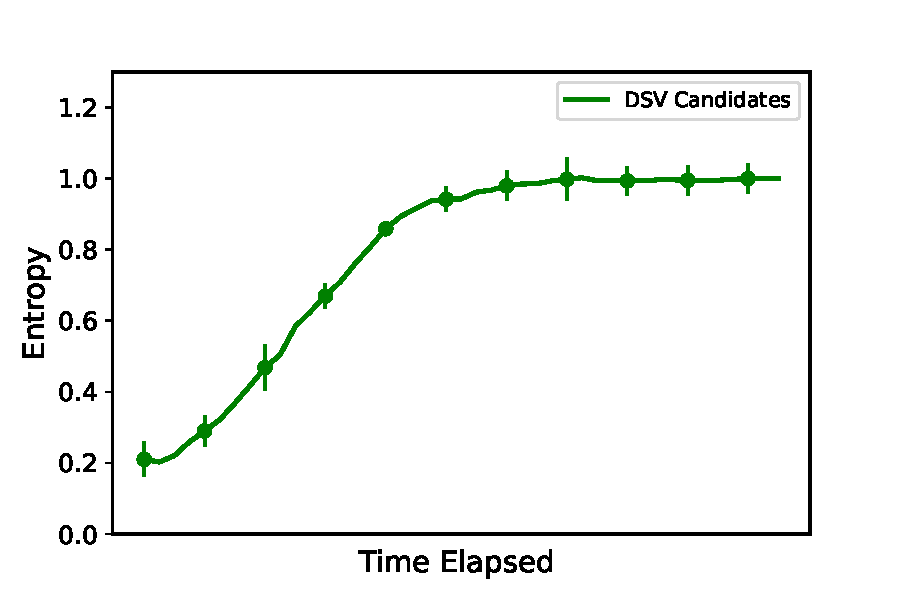
\includegraphics[width=\linewidth]{./figure/Entropy_DSV.pdf}
%     \caption{\nj{Entropy change of DSV candidates}}
%     \label{fig:lambda_entropy}
%   \end{subfigure}
%   \hfill
%   \begin{subfigure}[b]{3.4cm}
%     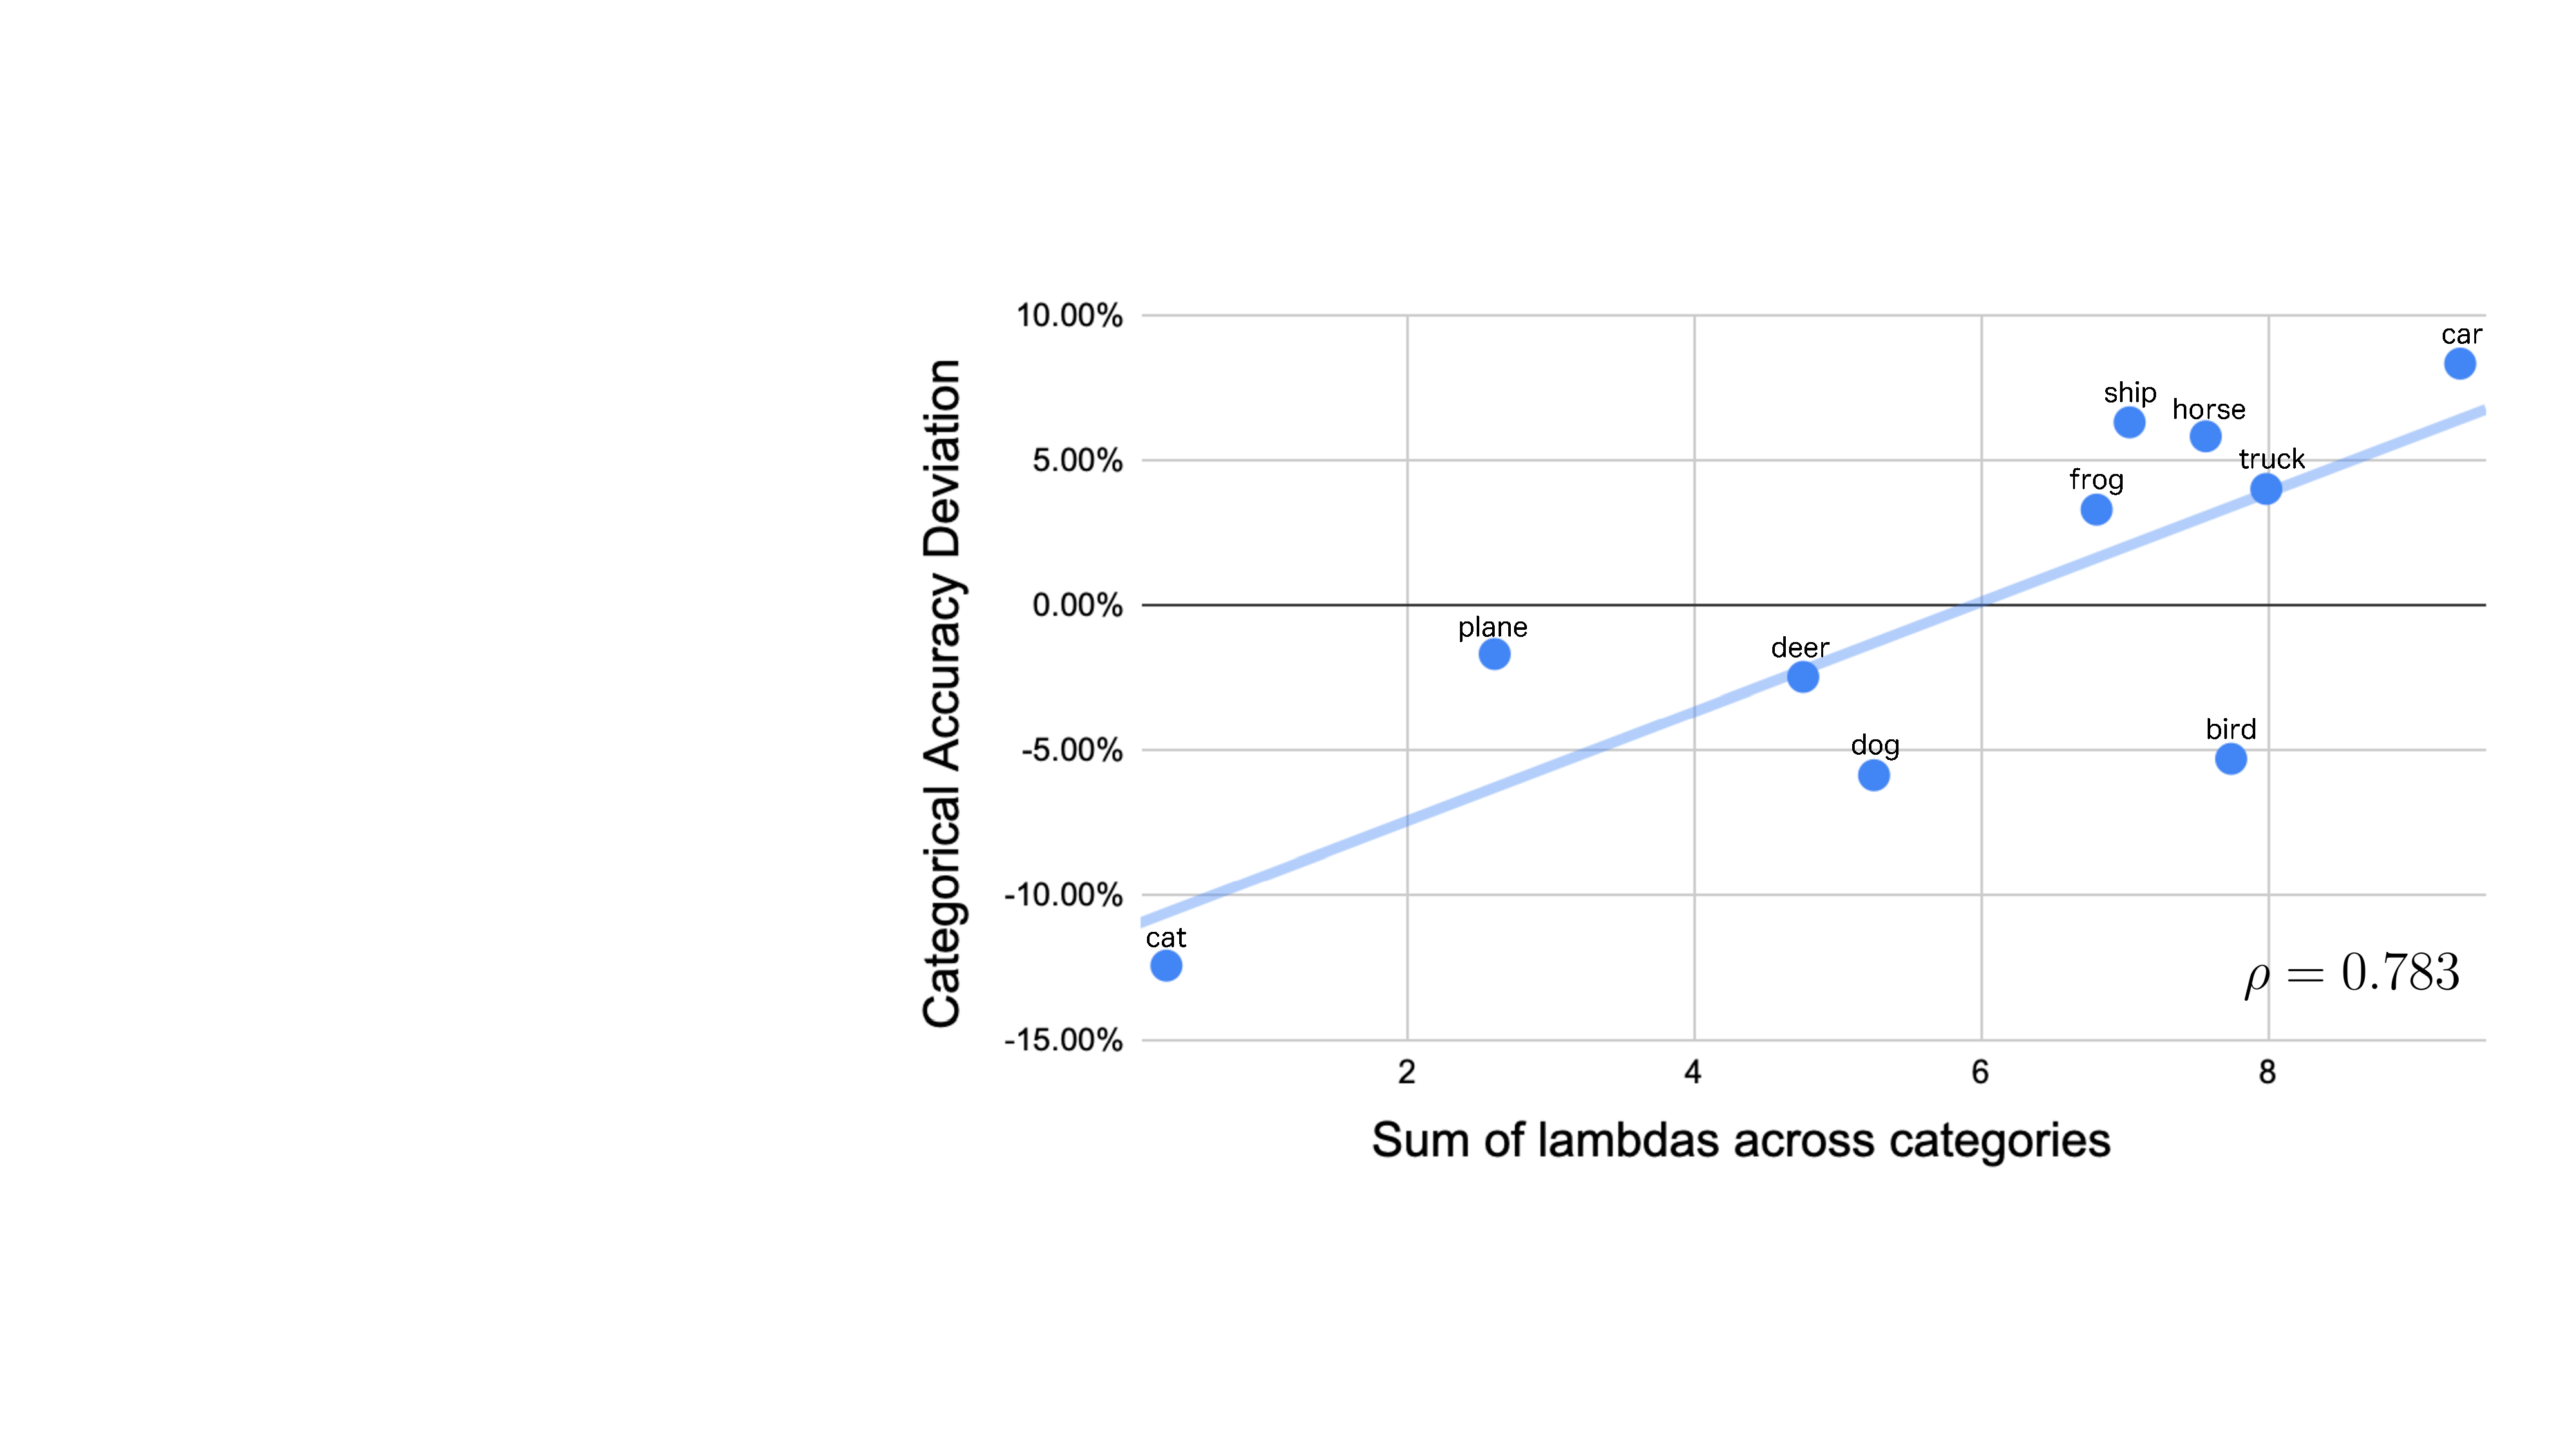
\includegraphics[width=\linewidth]{./figure/pearson.pdf}
%     \caption{Correlation between classwise mean test accuracy and \nj{the} sum of $\lambda$'s}
%     \label{fig:correlation}
%   \end{subfigure}
%   \caption{\nj{Figures showing different aspects of DSVs}}


\subsection{Unlocking the potential of classifier as generator with DeepKKT}


% \paragraph{DeepKKT in Transfer Learning}
\paragraph{\jh{Practical Model Inversion with DeepKKT}}


\begin{wrapfigure}{r}{6cm}
  \centering
  \vspace{-3mm}
   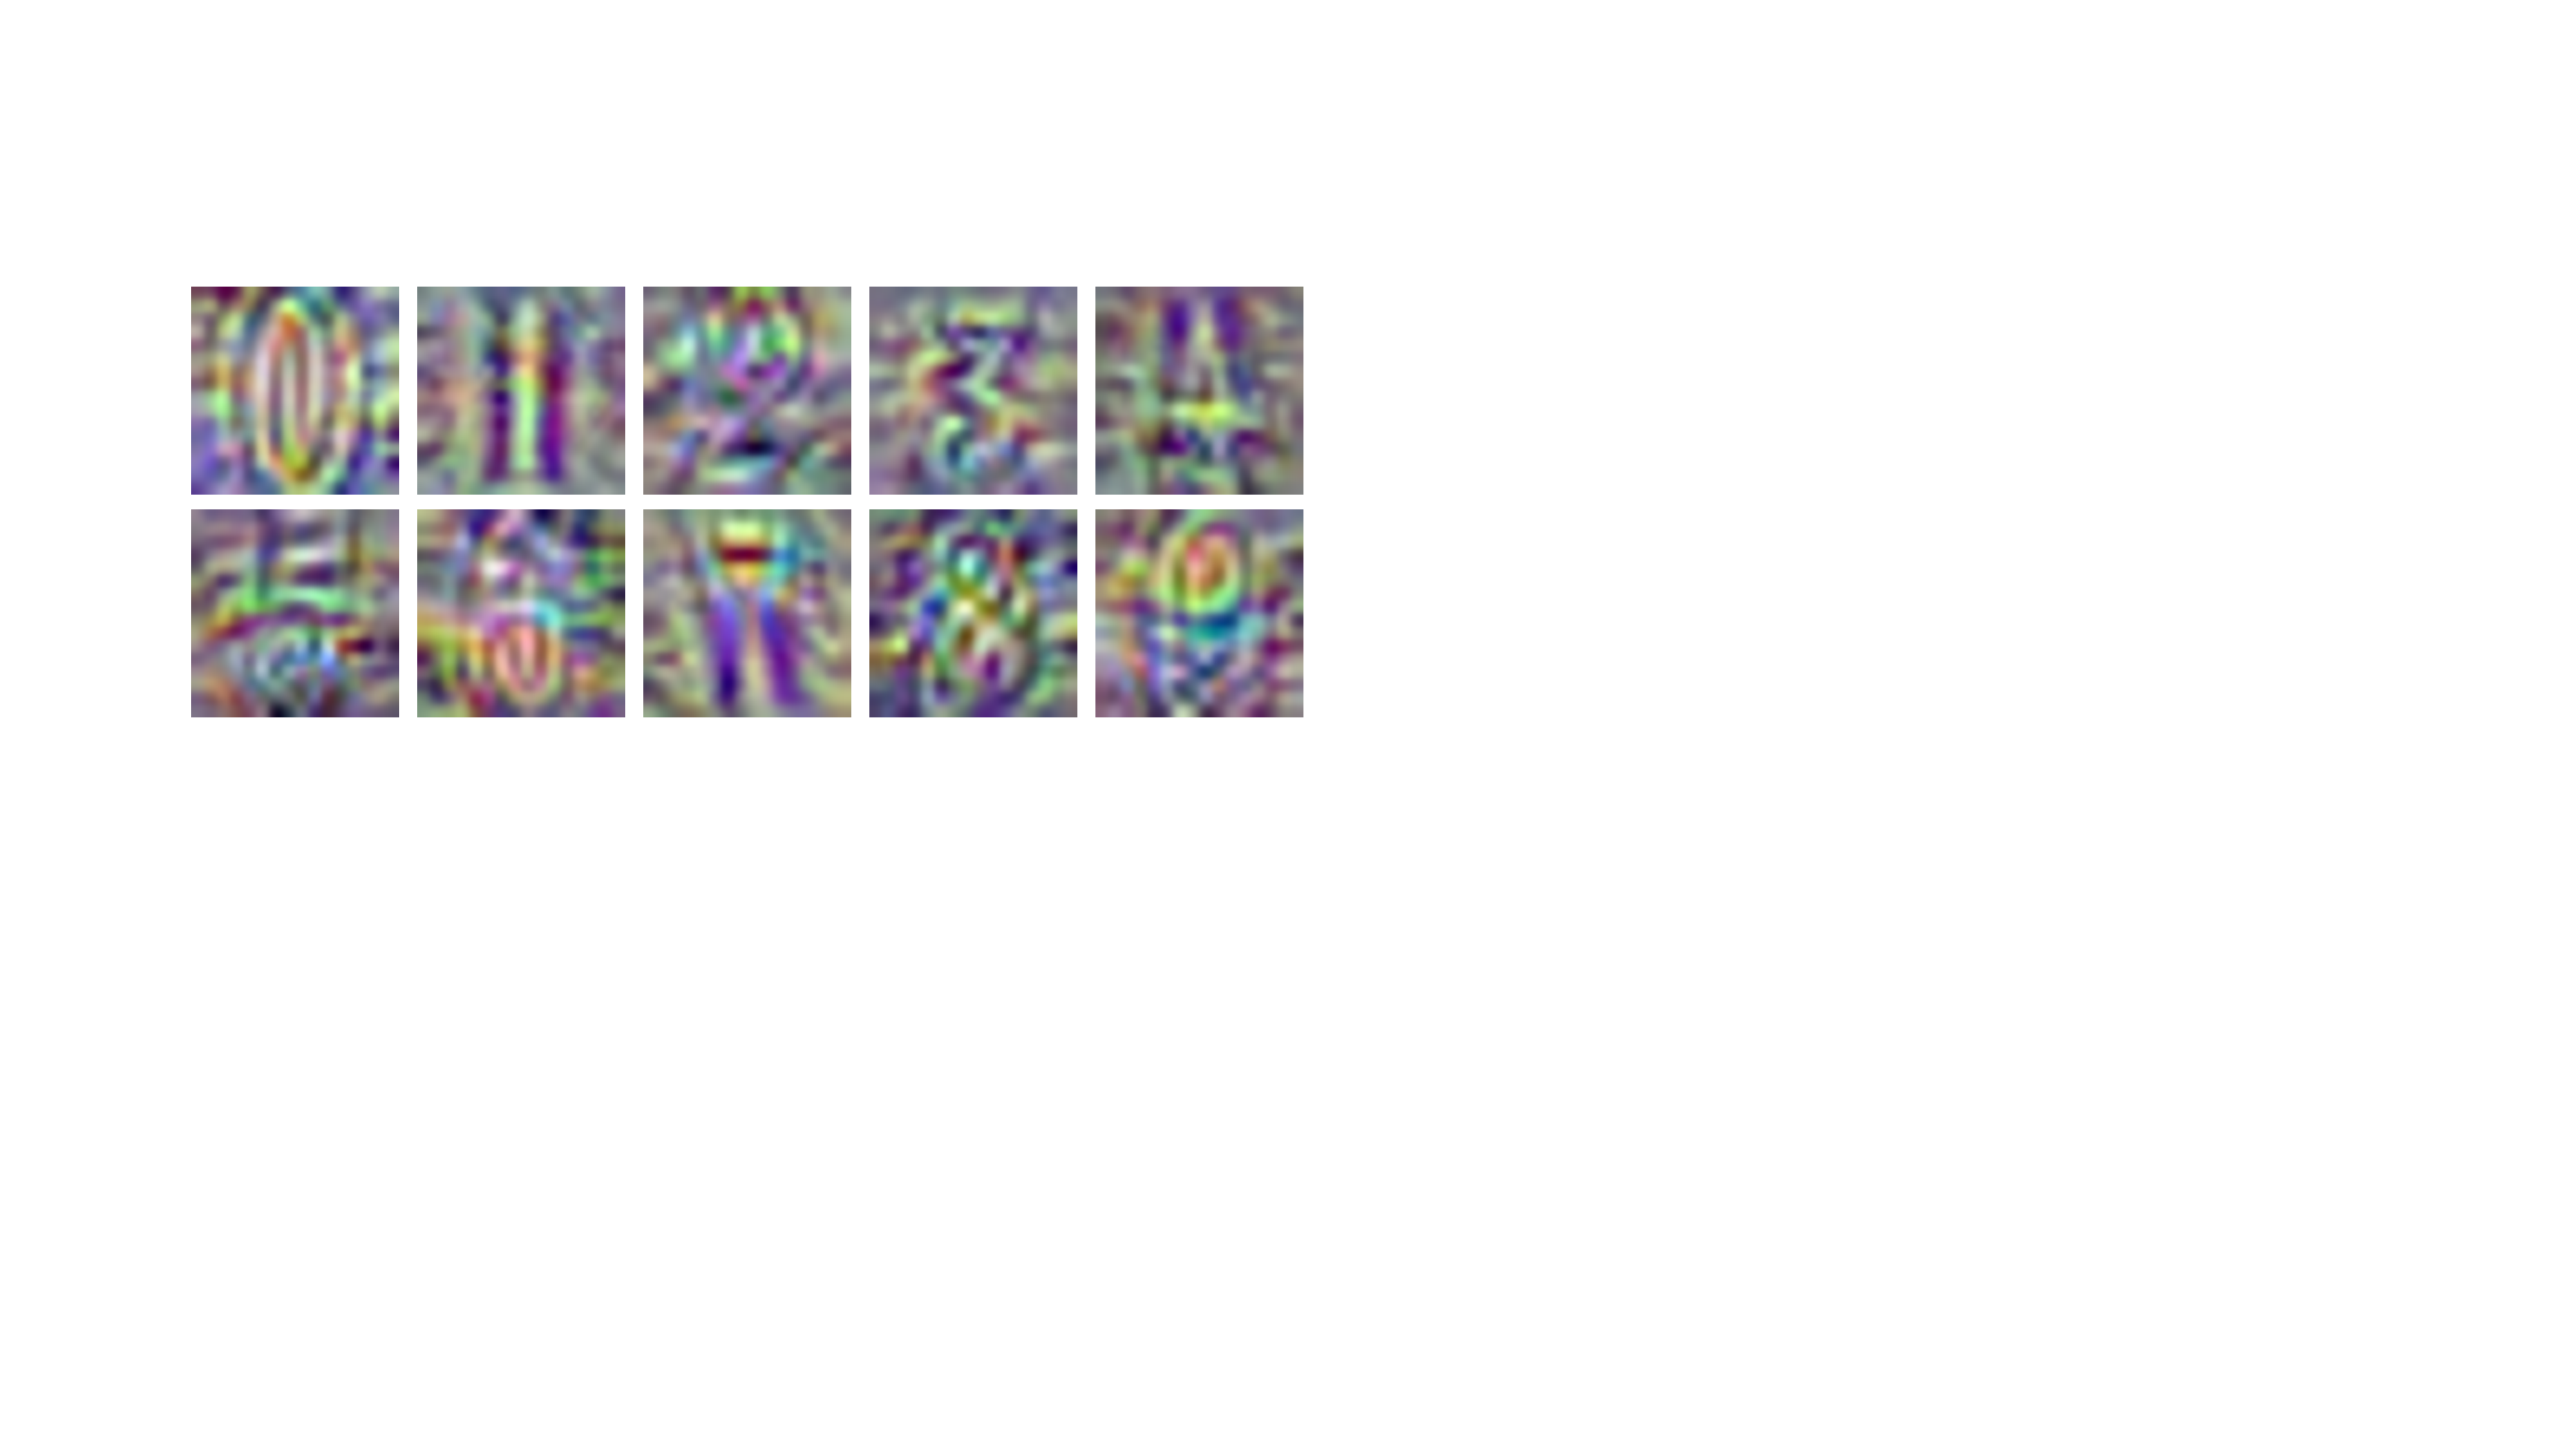
\includegraphics[width=6cm]{./figure/transfer.pdf}
   \caption{  \jh{DSVs generated by a model that underwent transfer learning from CIFAR-10 to SVHN. During transfer learning, only the last layer is updated \nj{by SVHN}.}}
   \label{fig:transfer}
% \end{figure}
\end{wrapfigure}


% It is crucial to acknowledge that practically, we do not fully-train whole parameter, we normally train partial parameters \ie transfer learning. DeepKKT works even this settings.
% \jh{It is important to acknowelogy that only partial parameters are learned practically such as transfer learning. In Fig.~\ref{fig:transfer}, DSVs are extracted solely from the last fully-connected layer of a model that has undergone transfer learning very that layer from the CIFAR-10 dataset to the SVHN dataset. Ev}
% \jh{In cloud environments or APIs, models are typically deployed with the belief that their black-box nature protects the sensitive information used during training. Users are generally assured that, despite the model being trained on sensitive data, they cannot infer this information. However, as demonstrated in Fig~\ref{fig:generated}, this belief is no longer valid. Fig~\ref{fig:transfer} further illustrates that model inversion remains feasible even in practical scenarios. This is especially evident in transfer learning scenarios, where only specific layers of a foundation model are fine-tuned. Remarkably, DeepKKT conditions enable model inversion even in these challenging environments, suggesting that they can be applied to a subset of the parameter space rather than the entire parameter space \ie more relaxed condition. Detailed explanations are provided in Sec.~\ref{sec:transfer}.}
% \jh{In cloud environments or APIs, models are deployed with the belief that their black-box nature protects the sensitive information used during training. Users are assured that, despite the model being trained on sensitive data, they cannot infer this information. 

\jh{In cloud environments or APIs, models are deployed with the belief that although they are sometimes trained with sensitive information, their black-box nature prevents users from inferring the data. This belief makes it possible to deploy sensitive models.}
However, as demonstrated in Fig~\ref{fig:generated}, this belief is no longer valid. Fig.~\ref{fig:transfer} further illustrates that model inversion remains feasible even in practical scenarios \nj{such as} transfer learning scenarios, where only specific layers of a foundation model are fine-tuned. Remarkably, DeepKKT conditions enable model inversion even in these challenging environments, suggesting that they can be applied to a subset of the parameter space rather than the entire parameter space \ie \nj{a} more relaxed condition.


%Detailed explanations are provided in Sec.~\ref{sec:transfer}.}


% \jh{In practice, instead of fully training all parameters, it is common to train only partial parameters through transfer learning. DeepKKT remains effective even in these settings.}
% In Fig.~\ref{fig:transfer}, DSVs are extracted solely from the last fully-connected layer of a model that has undergone transfer learning from the CIFAR-10 dataset to the SVHN dataset.
% Despite achieving \nj{an imperfect} training accuracy of 90$\%$ on the SVHN dataset (in an environment where the primal condition is not entirely satisfied), 
% we observe \nj{an} effective extraction of features \nj{that are} relevant to the SVHN dataset. This observation underscores two significant aspects: \hh{1)} The capability to independently extract DSVs by training only a subset of layers \nj{instead of} the entire layers, tailored to different datasets. \hh{2)} The robust applicability of relaxed DeepKKT conditions in practical and challenging environments where \nj{the} training accuracy does not completely reach 100$\%$.

\paragraph{Classifier as Latent generative model}
% 215, 417
% 787, 543
% 214, 896
% 594, 122

% \begin{figure}[h]
%   \centering
%    % \includegraphics[width=\linewidth]{./figure/ImageNet mix.pdf}
%    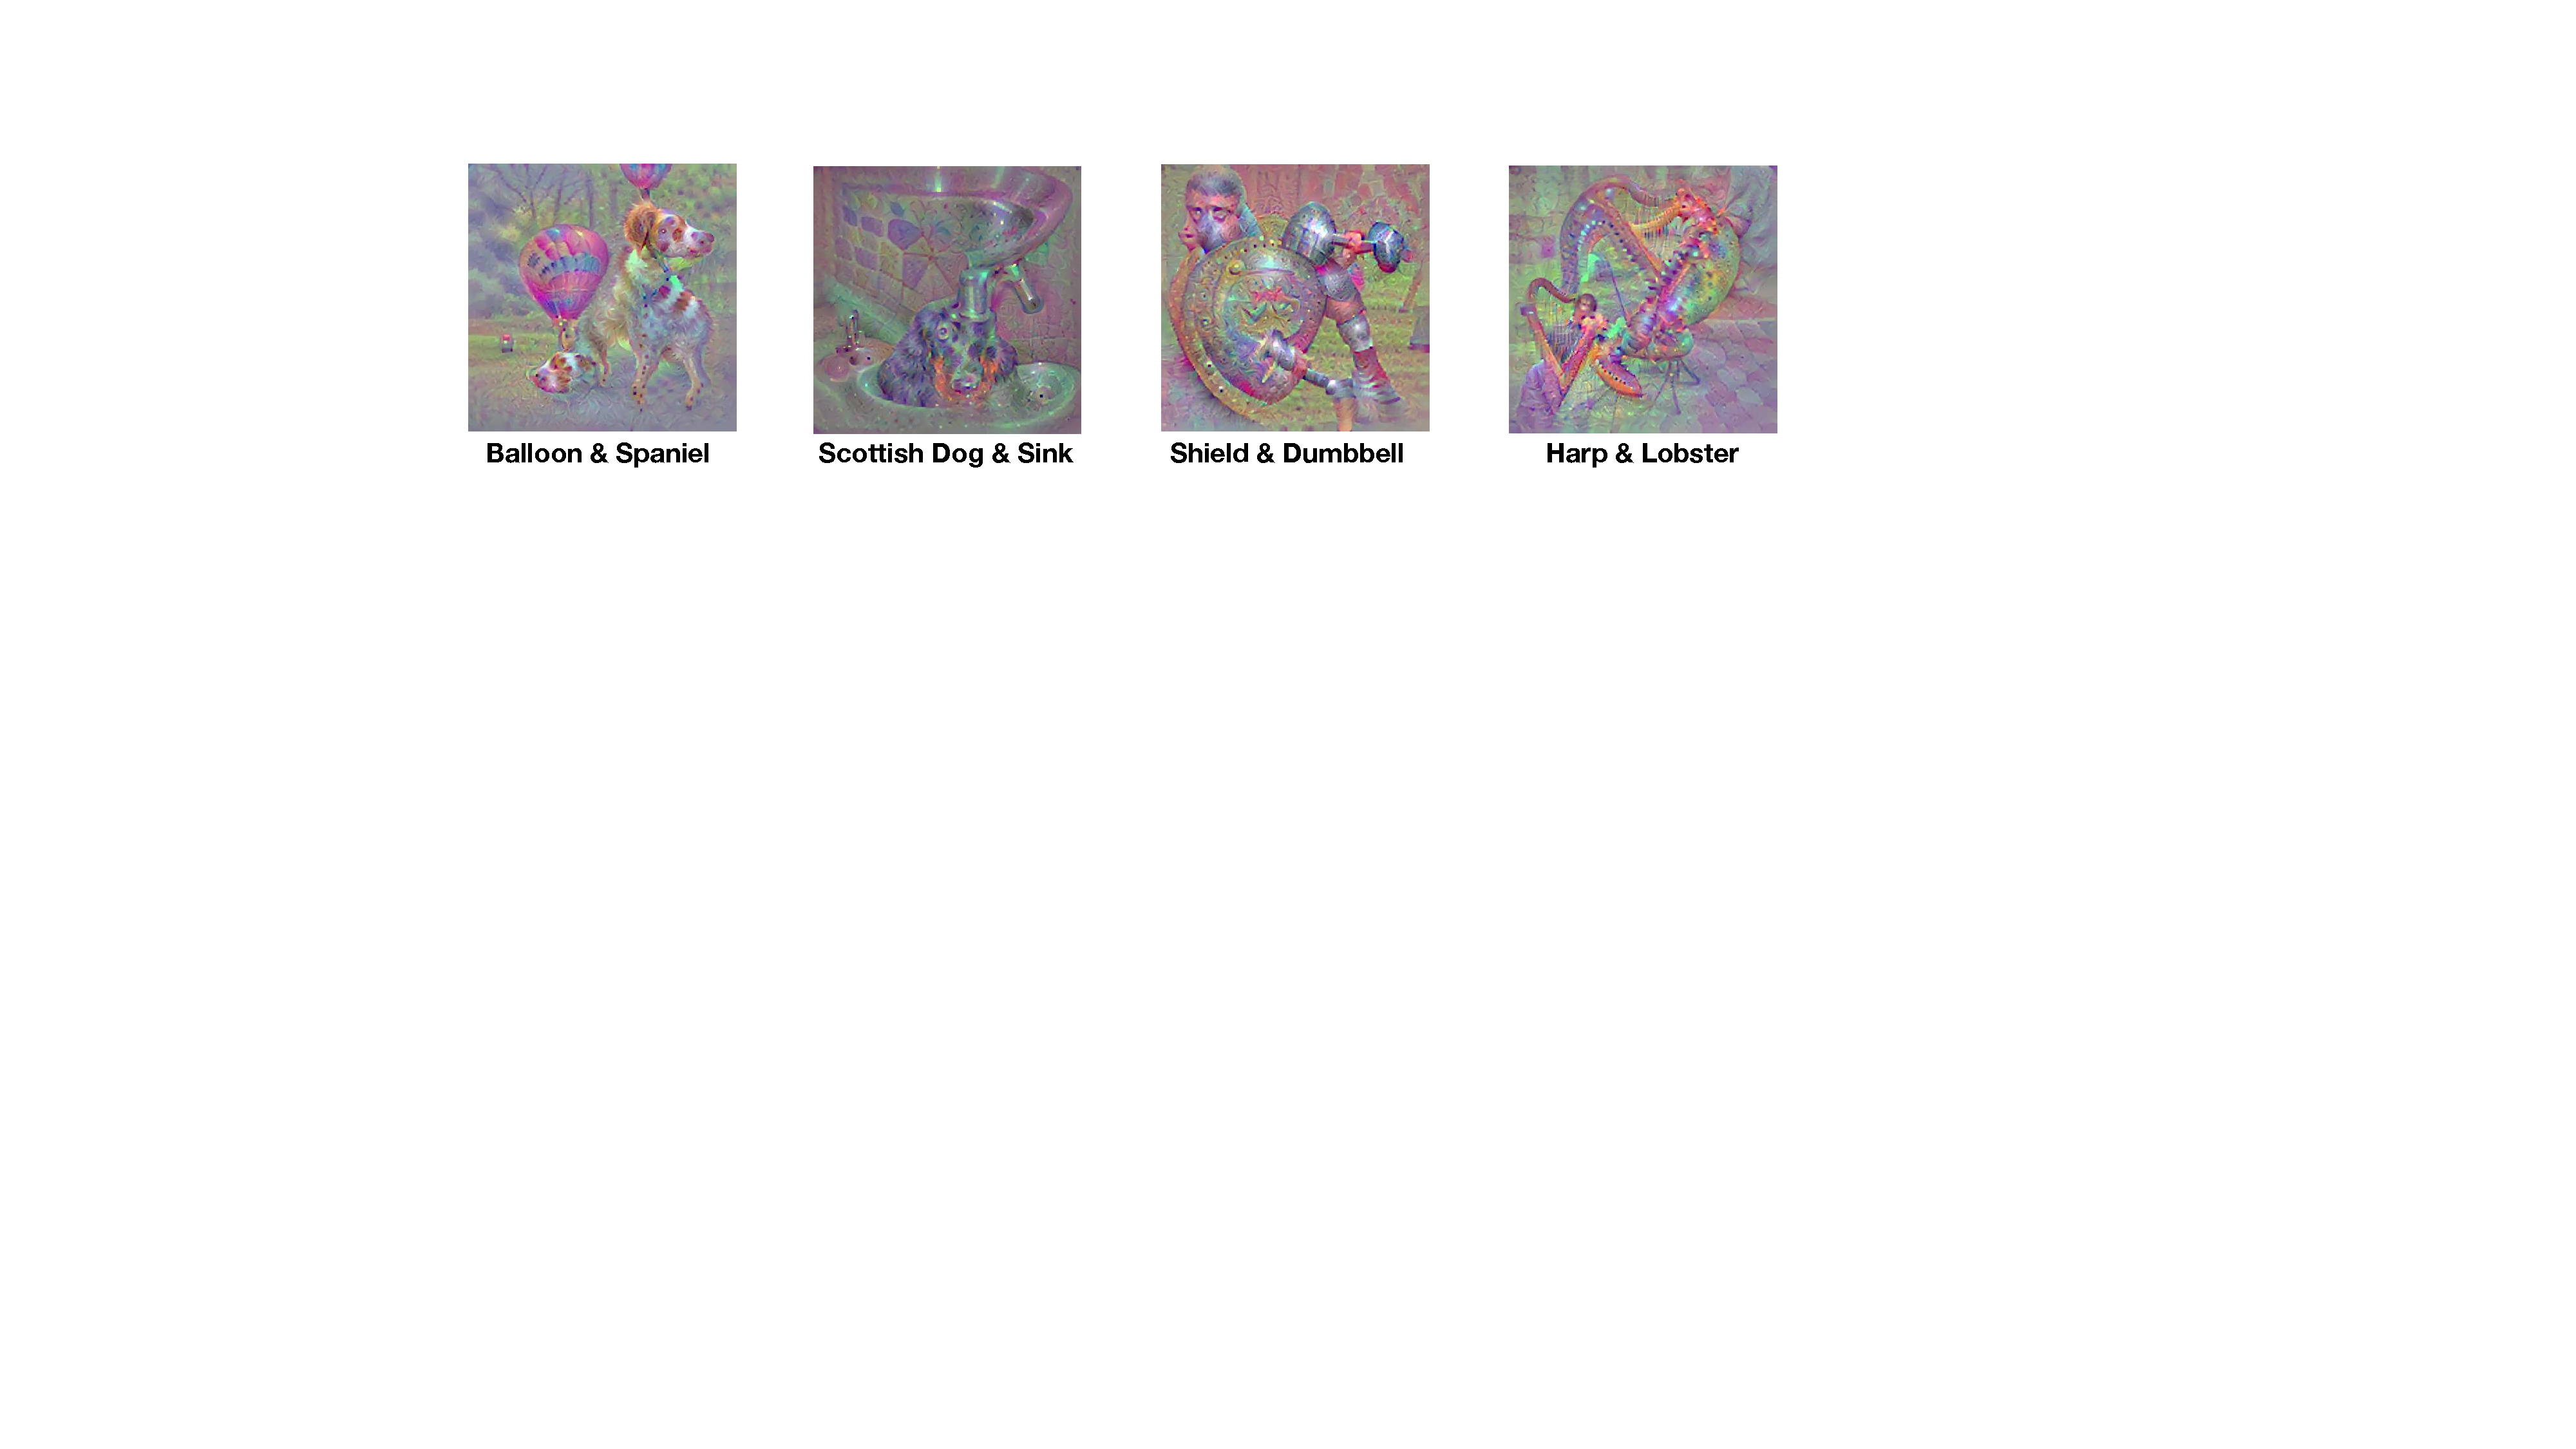
\includegraphics[width=\linewidth]{./figure/mixup_fig_compressed.pdf}
%    \caption{ \jh{Experiment on Latent Interpolation. Using labels as latent, DeepKKT condition generated unseen images. Generated image has } \nj{공간이 남으면 ballon, spaniel 각각 100\%로 만든 이미지도 보여주면 좋을 것 같음. } \jh{네 아예 latent interpolation 해보는것도 좋을것같아서 관련 코드 만들어서 돌려보고 있습니다!}}
%    \label{fig:latent}
% \end{figure}
% \begin{figure}[h]
%   \centering
%    % \includegraphics[width=\linewidth]{./figure/ImageNet mix.pdf}
%    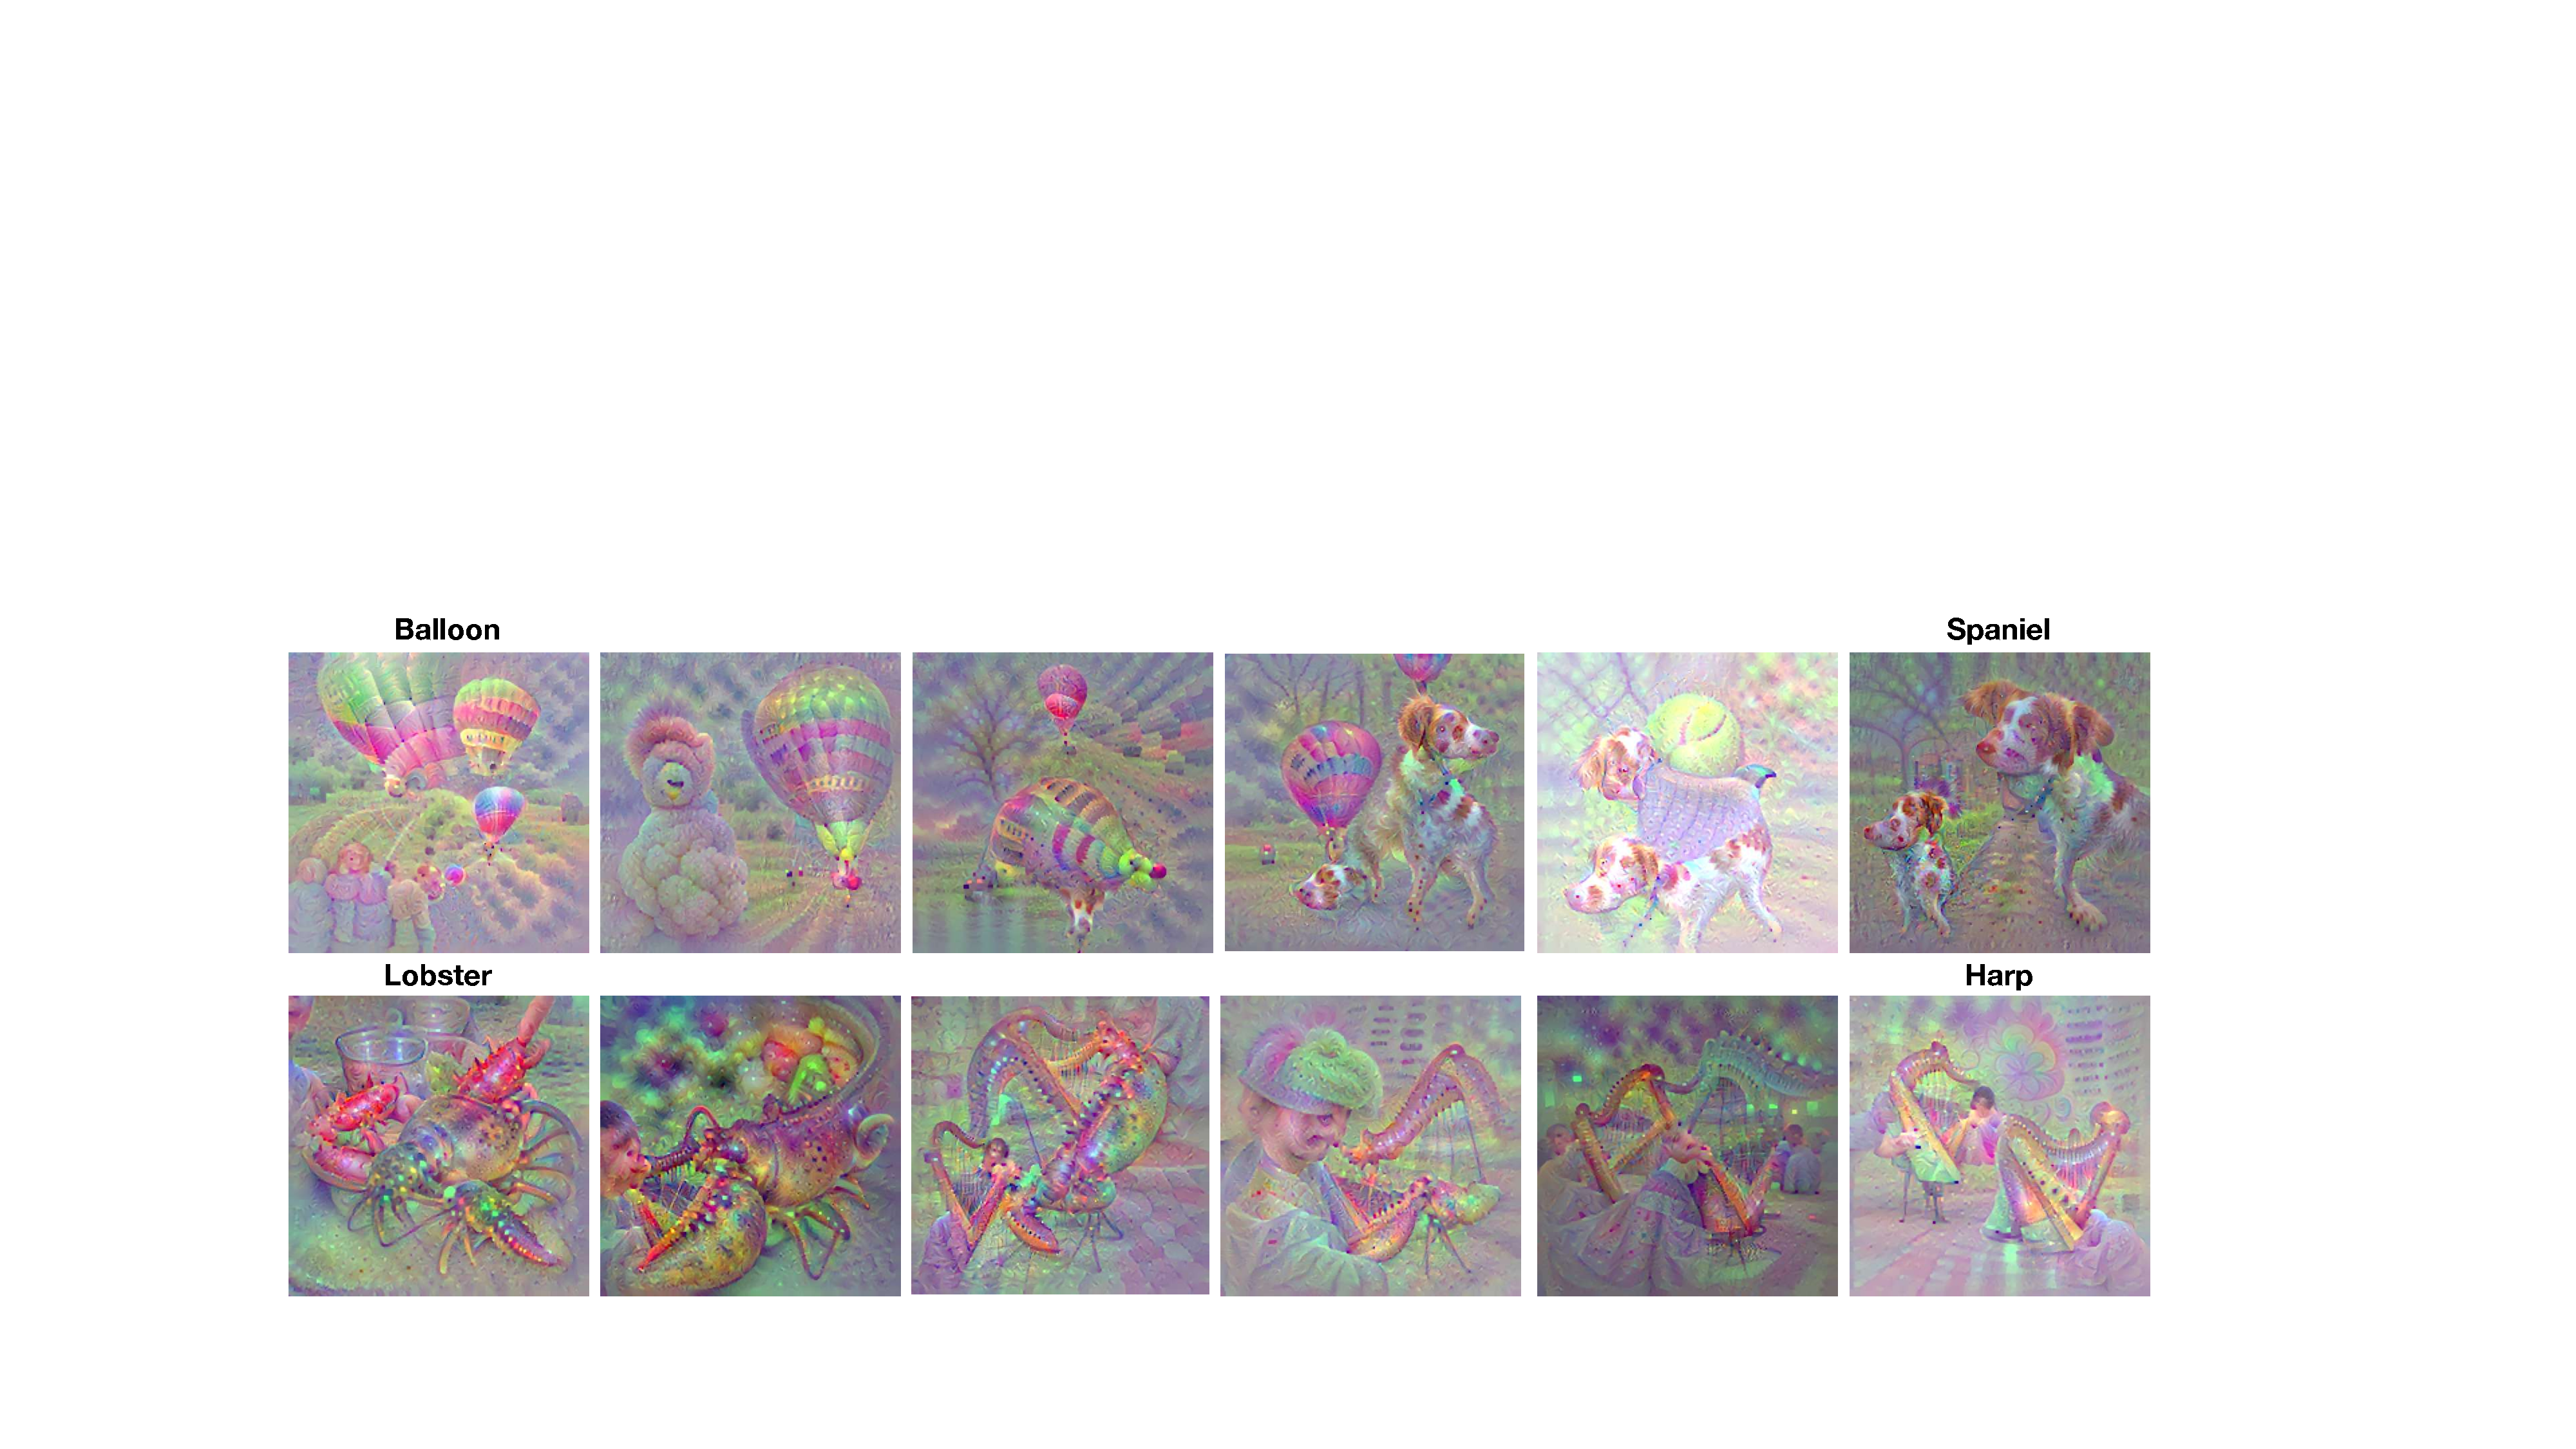
\includegraphics[width=\linewidth]{./figure/interpolation_fig_compressed.pdf}
%    \caption{ \jh{Experiment on Latent Interpolation. Using labels as latent, DeepKKT condition generated unseen images. Generated image has } \nj{공간이 남으면 ballon, spaniel 각각 100\%로 만든 이미지도 보여주면 좋을 것 같음. } \jh{네 아예 latent interpolation 해보는것도 좋을것같아서 관련 코드 만들어서 돌려보고 있습니다!}}
%    \label{fig:latent}
% \end{figure}
% \begin{figure}[h]
%   \centering
%   \begin{minipage}{\linewidth}
%     \centering
%     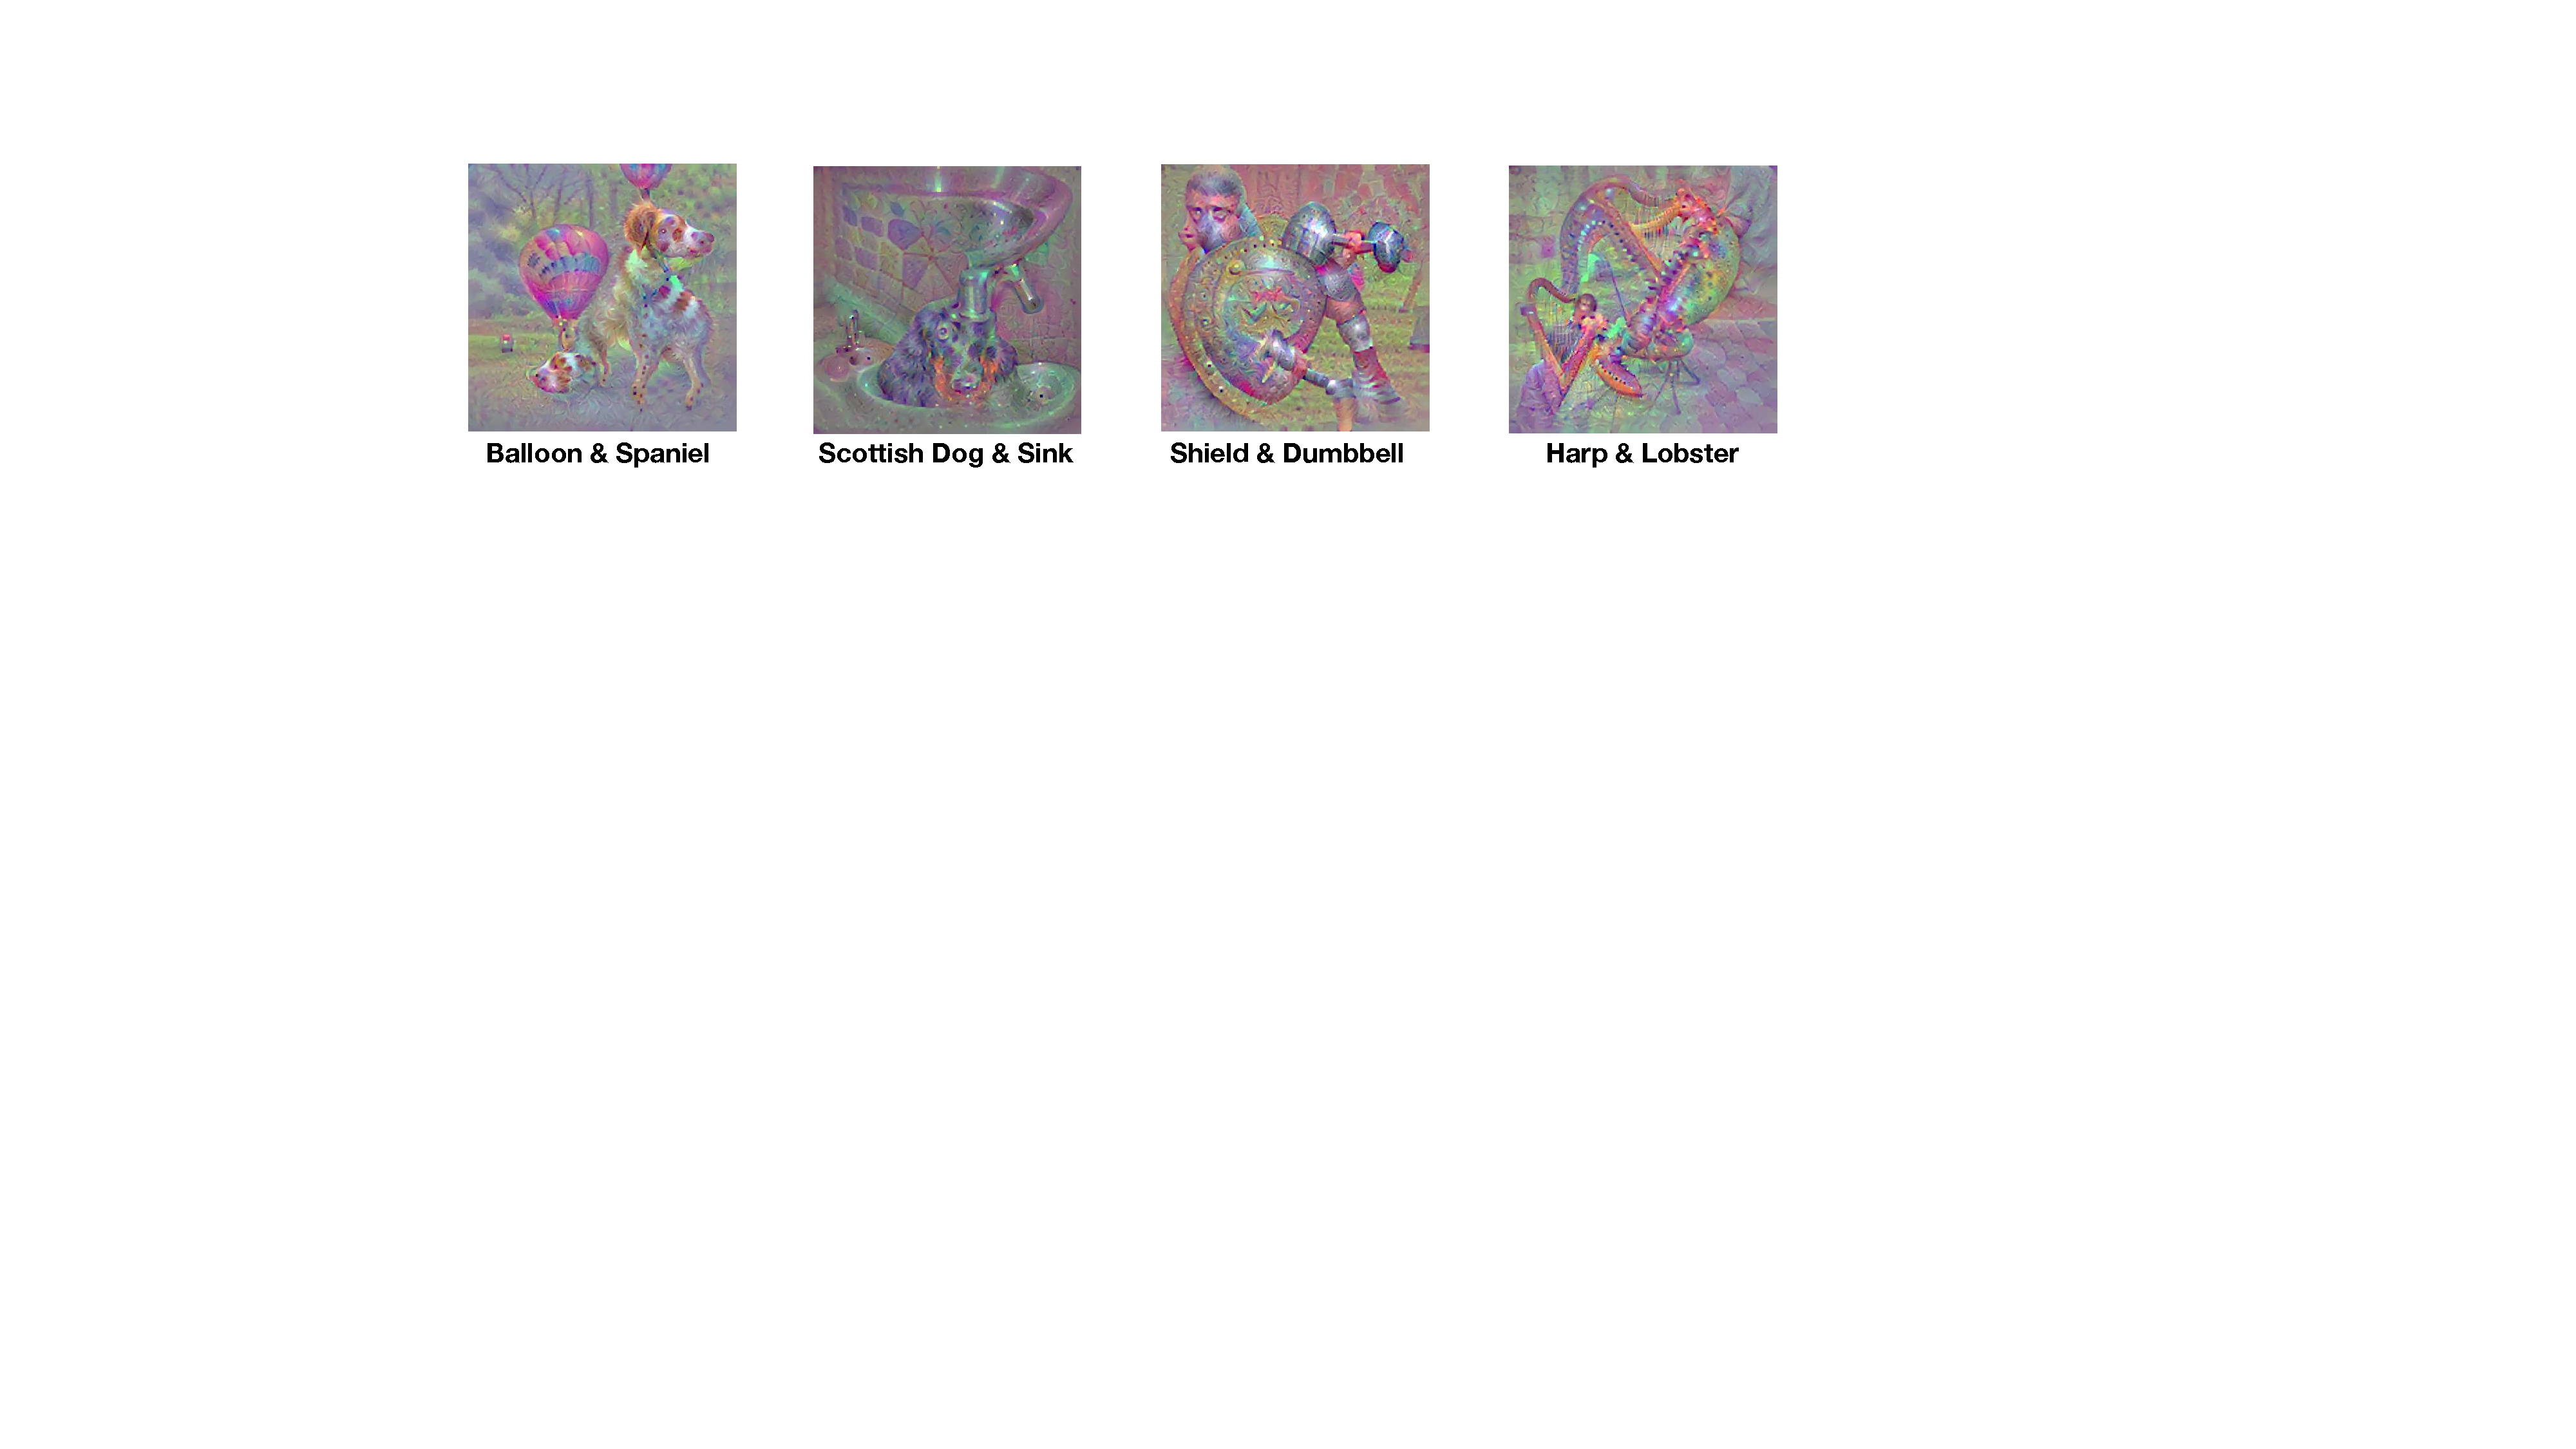
\includegraphics[width=\linewidth]{./figure/mixup_fig_compressed.pdf}
%     \caption{Experiment on Latent Interpolation. Using labels as latent, DeepKKT condition generated unseen images. Generated image has.}
%     \label{fig:latent1}
%   \end{minipage}
  
%   \vspace{1cm} % Adjust the vertical space between the images as needed
  
%   \begin{minipage}{\linewidth}
%     \centering
%     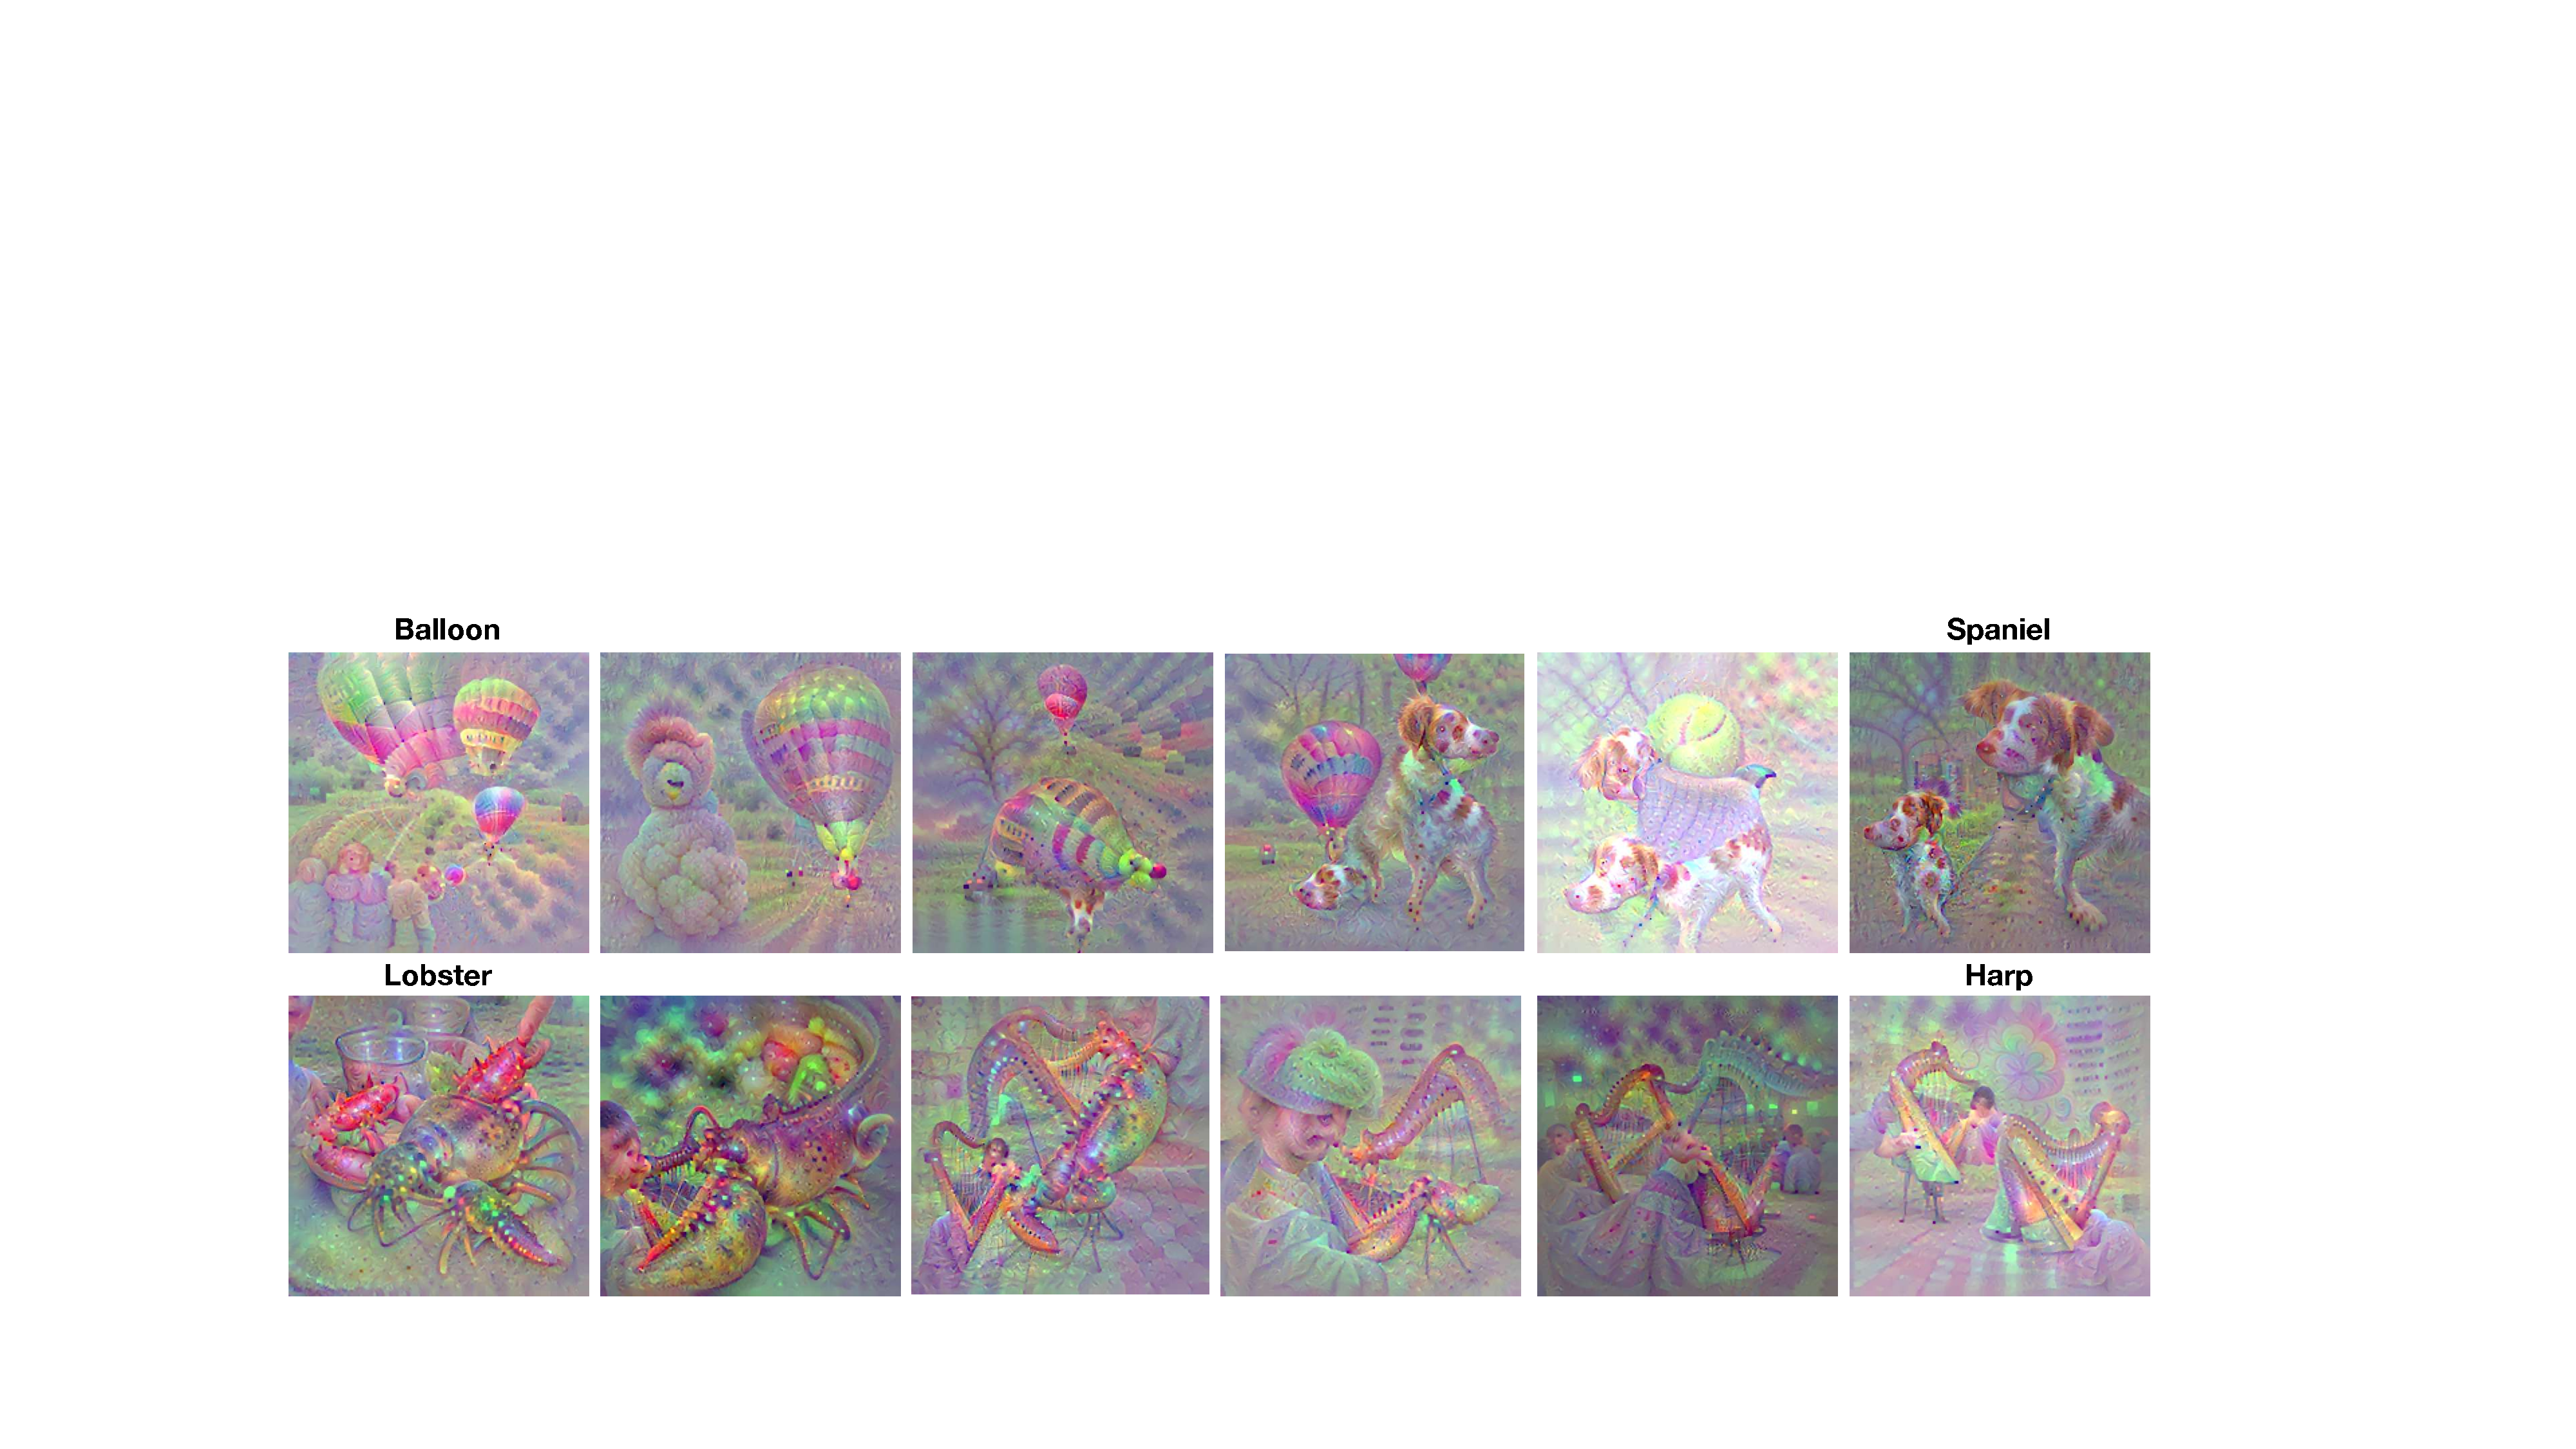
\includegraphics[width=\linewidth]{./figure/interpolation_fig_compressed.pdf}
%     \caption{Experiment on Latent Interpolation. Using labels as latent, DeepKKT condition generated unseen images. Generated image has.}
%     \label{fig:latent2}
%   \end{minipage}
% \end{figure}



% \jh{Take }
% \jh{As each DSV is a representative of decision criterion of certain target, we arbitary generated target in accrords to the size of classifier. The fact DSVs are genarated accords to the target, it implies that the image is generated using the target as latent. Meaning, we can use general classifier as deep latent generation model with using targets as latent! Fig.~\ref{fig:latent} shows striking results, when we generate DSVs for soft classes \ie soft targets from two classes. It act as a latent interpolation of generative models. This is interesting phenomenon concerning its optimization procedure is similar to diffusion model.}\\
% \hh{Generally the diffusion process could be seperated into two terms : the denoising term and a guidance term.  The guidance term enforces the images to go towards the representing classes which does the same role as the primal condition. 
% For the stationarity condition, its gradient with respect to the corresponding DSV $x_i$ could be represented as $$\nabla_{x_i} L_{\text{stat}} =\nabla D(\theta^*, -\sum_{i=1}^n \lambda_i \nabla_\theta L(\Phi(x_i;\theta^*), y_i)) \cdot \lambda_i \nabla_{x_i}(\nabla_\theta L(\Phi(x_i;\theta^*), y_i))$$ due to the chain rule. $\lambda_i \nabla_{x_i}(\nabla_\theta L(\Phi(x_i;\theta^*), y_i))$ denotes the Hessian of the loss function, while  $\nabla D(\theta^*, -\sum_{i=1}^n \lambda_i \nabla_\theta L(\Phi(x_i;\theta^*), y_i))$  denotes the derivative of distance function. Therefore $\nabla_{x_i} L_{\text{stat}}$ is the direction where $x_i$ minimizes the loss gradient $\nabla_\theta L$ by the scale of $\nabla D$, which is the direction of the optimal DSV should be. This serves a similar role to the score function $\nabla_x \log p(x_t)$ in diffusion models.
% \begin{equation}
% \theta^* = - \sum_{i=1}^n \lambda_i \nabla_{\theta^*} L(\Phi(x_i; \theta^*), y_i).
% \end{equation}



% \jh{Generation Procedure through DeepKKT condition can be written as follows}
% \begin{equation}
% x_{t+1} = x_{t} + \alpha \cdot \left( \nabla_x L_{\text{stat}}(A(x)) + \beta \nabla_x L_{\text{primal}}(A(x) \right)
% \end{equation}
% \begin{equation}
% x_{t+1} = x_t + \epsilon_t \cdot \left( \nabla_x \log p(x_t) + \lambda \nabla_x \log p(y | x_t) \right)
% \end{equation}

\jh{Considering the impressive capabilities of DSVs in the \nj{image} generation domain, and the geometric interpretation that DSVs \nj{are samples near the decision} boundaries, %$\partial \mathcal{M}$, 
% \jh{Considering the impressive capabilities of DSVs in the \nj{image} generation domain, and the geometric r}
%and the geometric interpretation that DSVs \nj{are samples near the decision} boundaries,} %$\partial \mathcal{M}$, 
% it is \nj{noted} that \nj{enforcing the DeepKKT condition} resembles the \nj{diffusion process.} In each iteration, the DSV develops according to the DeepKKT condition as follows: %\nj{(9)식에서는 beta가 없고 아래 식에서는 9식의 마지막 두 term이 없음.}
it is \nj{noted} that \nj{enforcing the DeepKKT condition} resembles the \nj{diffusion process.} In each iteration, the DSV develops through the DeepKKT condition as follows: %\nj{(9)식에서는 beta가 없고 아래 식에서는 9식의 마지막 두 term이 없음.}
}
\begin{equation}
x_{t+1} = x_{t} - \nj{\eta} \cdot \left( [ \nabla_x L_{\text{stat}}(\mathcal{A}(x_t)) +  \beta_2 L_{\text{tot}}(x_t) + \beta_3 L_{\text{norm}}(x_t) ]  + \beta_1 \nabla_x L_{\text{primal}}(\mathcal{A}(x_t)) \right).
\label{eq:update}
\end{equation}
\nj{This is similar to the generalized form} of the \nj{score-based} diffusion process:
\begin{equation}
x_{t+1} = x_t + \epsilon_t \cdot \left( \nabla_x \log p(x_t) + \gamma \nabla_x \log p(y | x_t) \right).
\end{equation}


% \nj{The first three loss terms in Eq.~(\ref{eq:update}) correspond to maximizing the score ($\nabla_x \log p(x_t)$) while the primal feasibility term in the last corresponds to the guidance term $(\gamma \nabla_x \log p(y | x_t))$. As observed in Fig.~\ref{fig:primalstat}, when only the primal loss term is provided, meaningful \nj{DSV} samples are not generated. \jh{Indicating other losses (stationarity and manifold term) act as score function.}}
% \jh{From this perspective, \nj{an \textbf{arbitrarily assigned label} $y$ can be exploited as a latent in guidence.}}
\begin{wrapfigure}{r}{6cm}
  \centering
   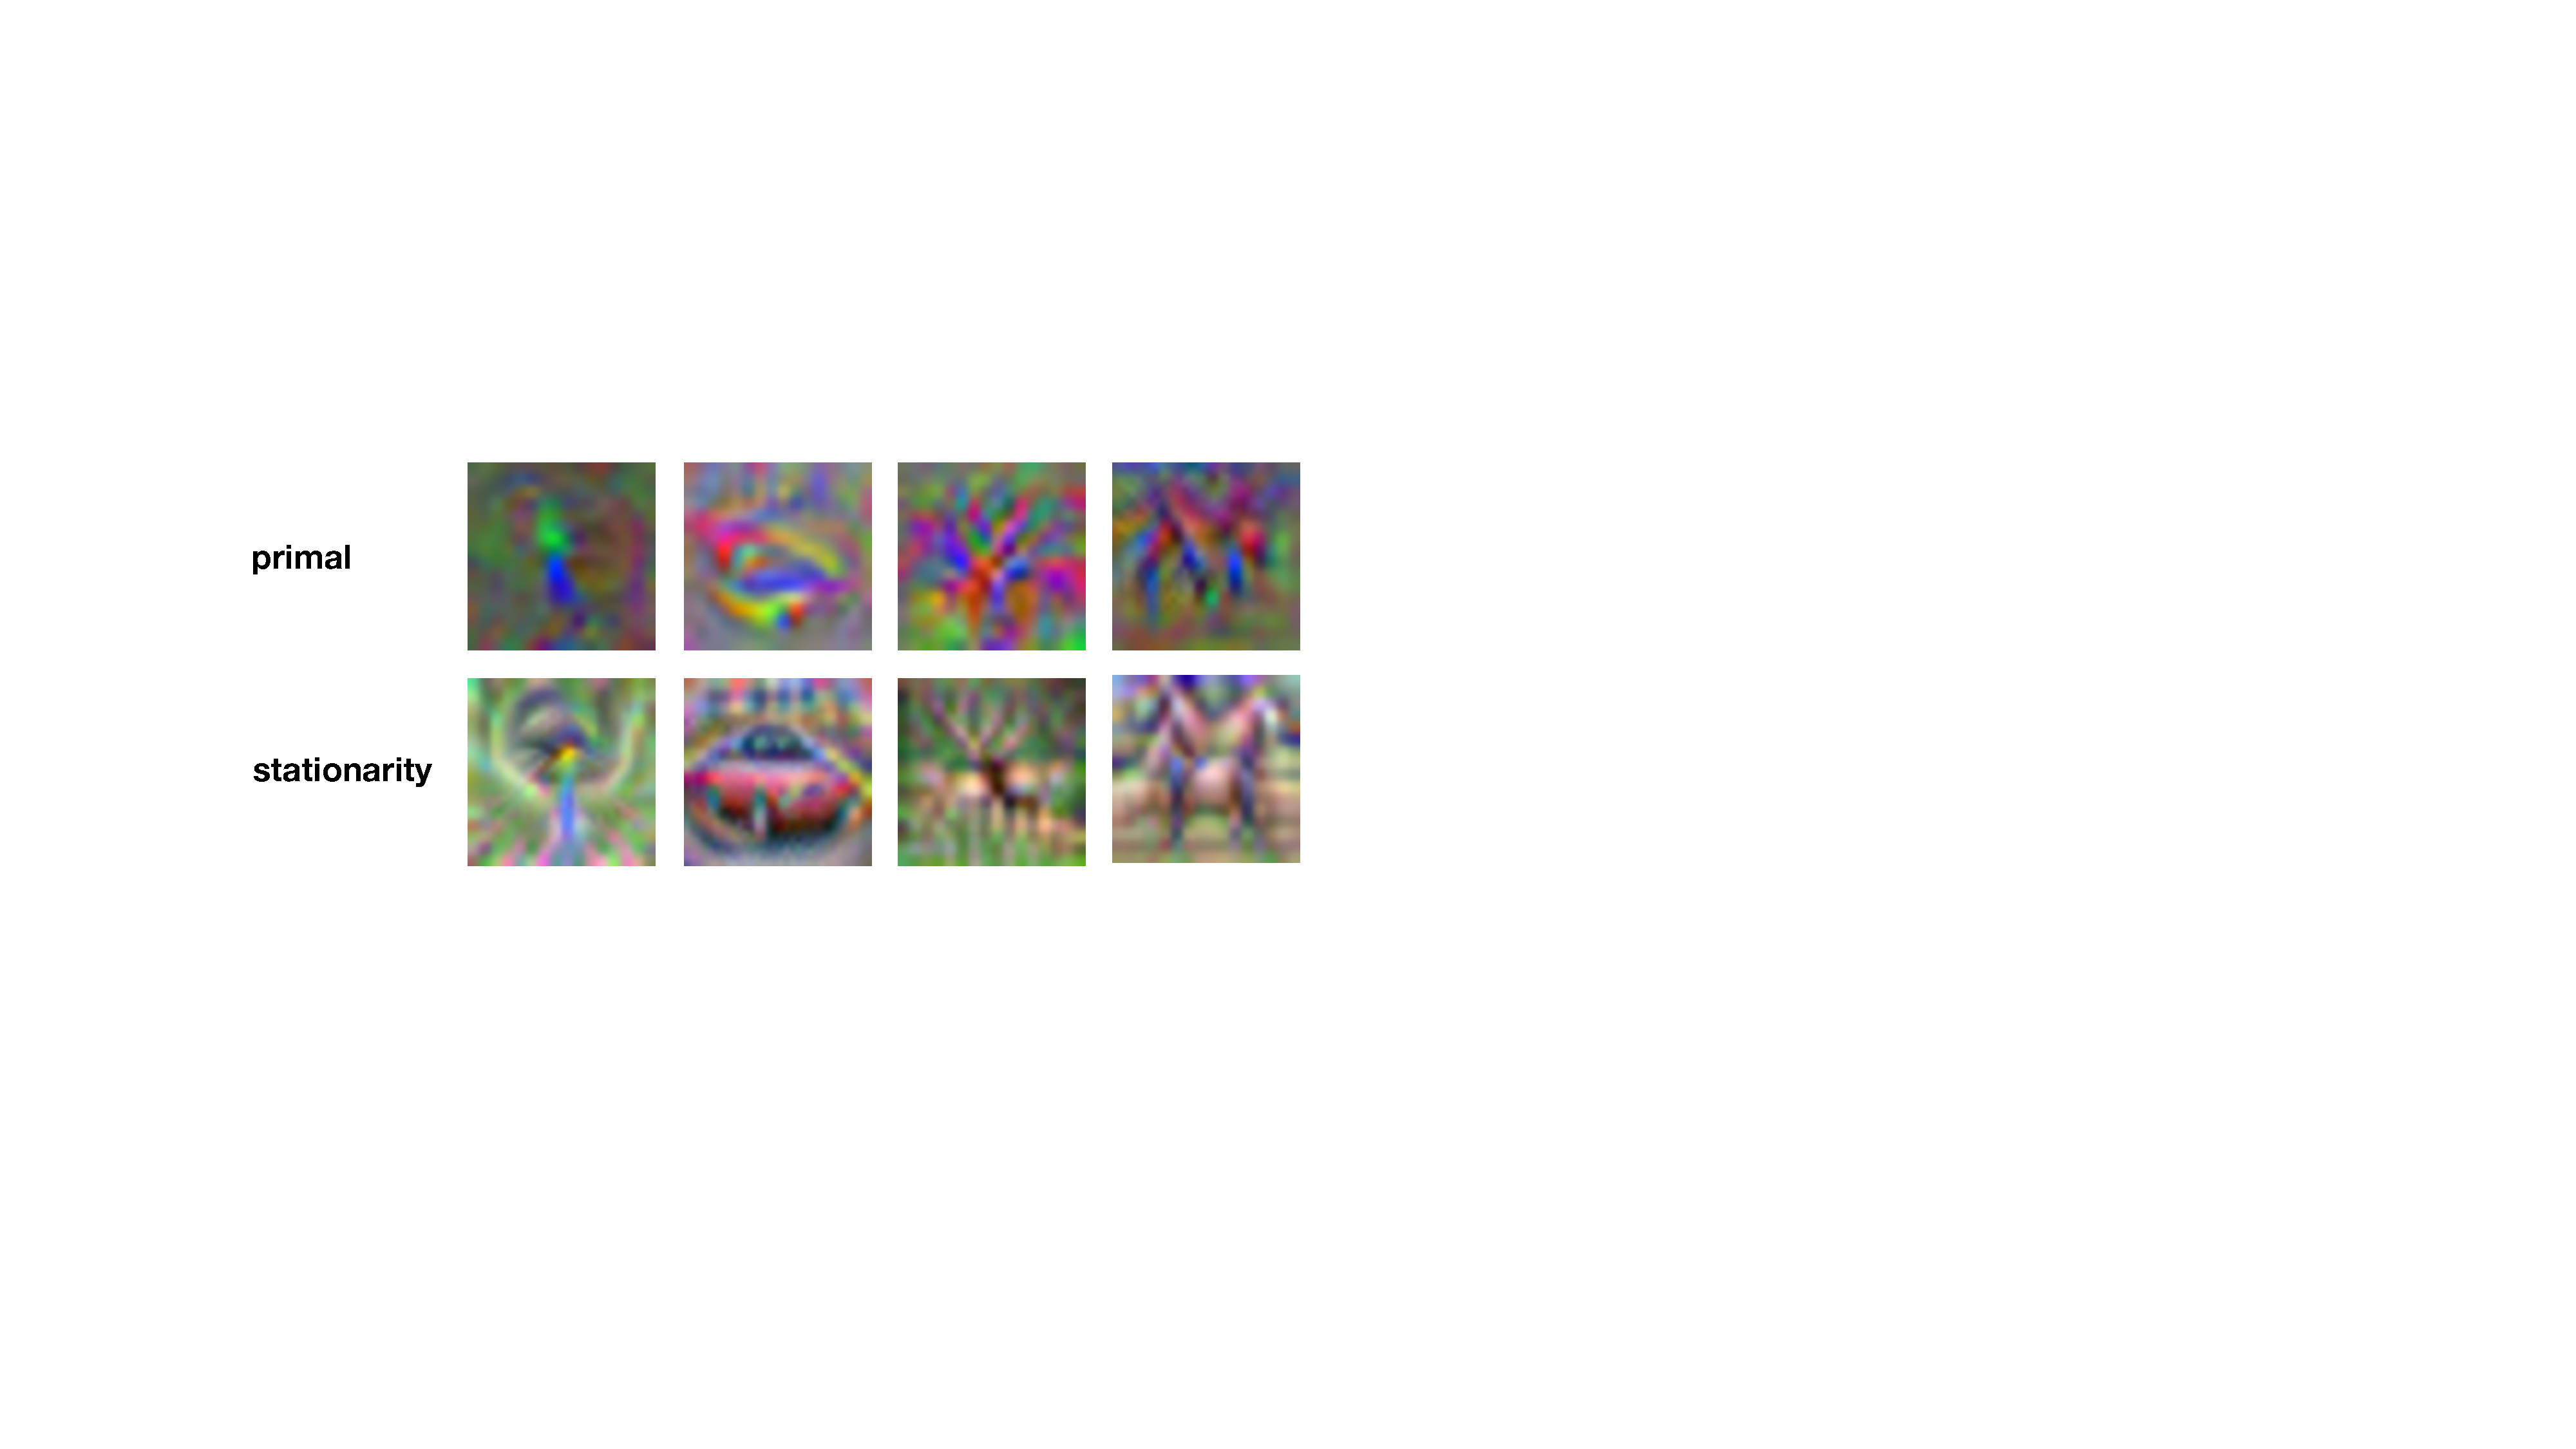
\includegraphics[width=\linewidth]{./figure/primalstat.pdf}
   \caption{Results showing \jh{DeepKKT} images created solely by the primal condition or by the stationary condition. \jh{\nj{A sole usage} of the primal condition shows low fidelity.}}
   \label{fig:primalstat}
   \vspace{-5mm}
% \end{figure}
\end{wrapfigure}
\jh{The first three loss terms in Eq.~(\ref{eq:update}) aim to maximize the score ($\nabla_x \log p(x_t)$), while the last term, the primal feasibility term, corresponds to the guidance term ($\gamma \nabla_x \log p(y | x_t)$). As shown in Fig.~\ref{fig:primalstat}, when only the primal loss term is used, meaningful DSV samples are not generated. This indicates that the other losses (stationarity and manifold terms) function update the image towards manifold \ie score function.
From this perspective, an arbitrarily assigned label $y$ can be used as a latent variable for guidance.}

%\jh{as guidance-term-only diffusion model does, indicating that the roles of the two loss terms are very similar}}. 
% \jh{From this perspective, \nj{an \textbf{arbitrarily assigned label} $y$ can be exploited as a latent in guidence.} \ie, classifier guidance}.
%From this perspective, \nj{an \textbf{arbitrarily assigned label} $y$ can be exploited as a latent} \jh{\ie, classifier guidance}.}

\begin{figure}[t]
  \centering
  \begin{subfigure}[b]{\linewidth}
    \centering
    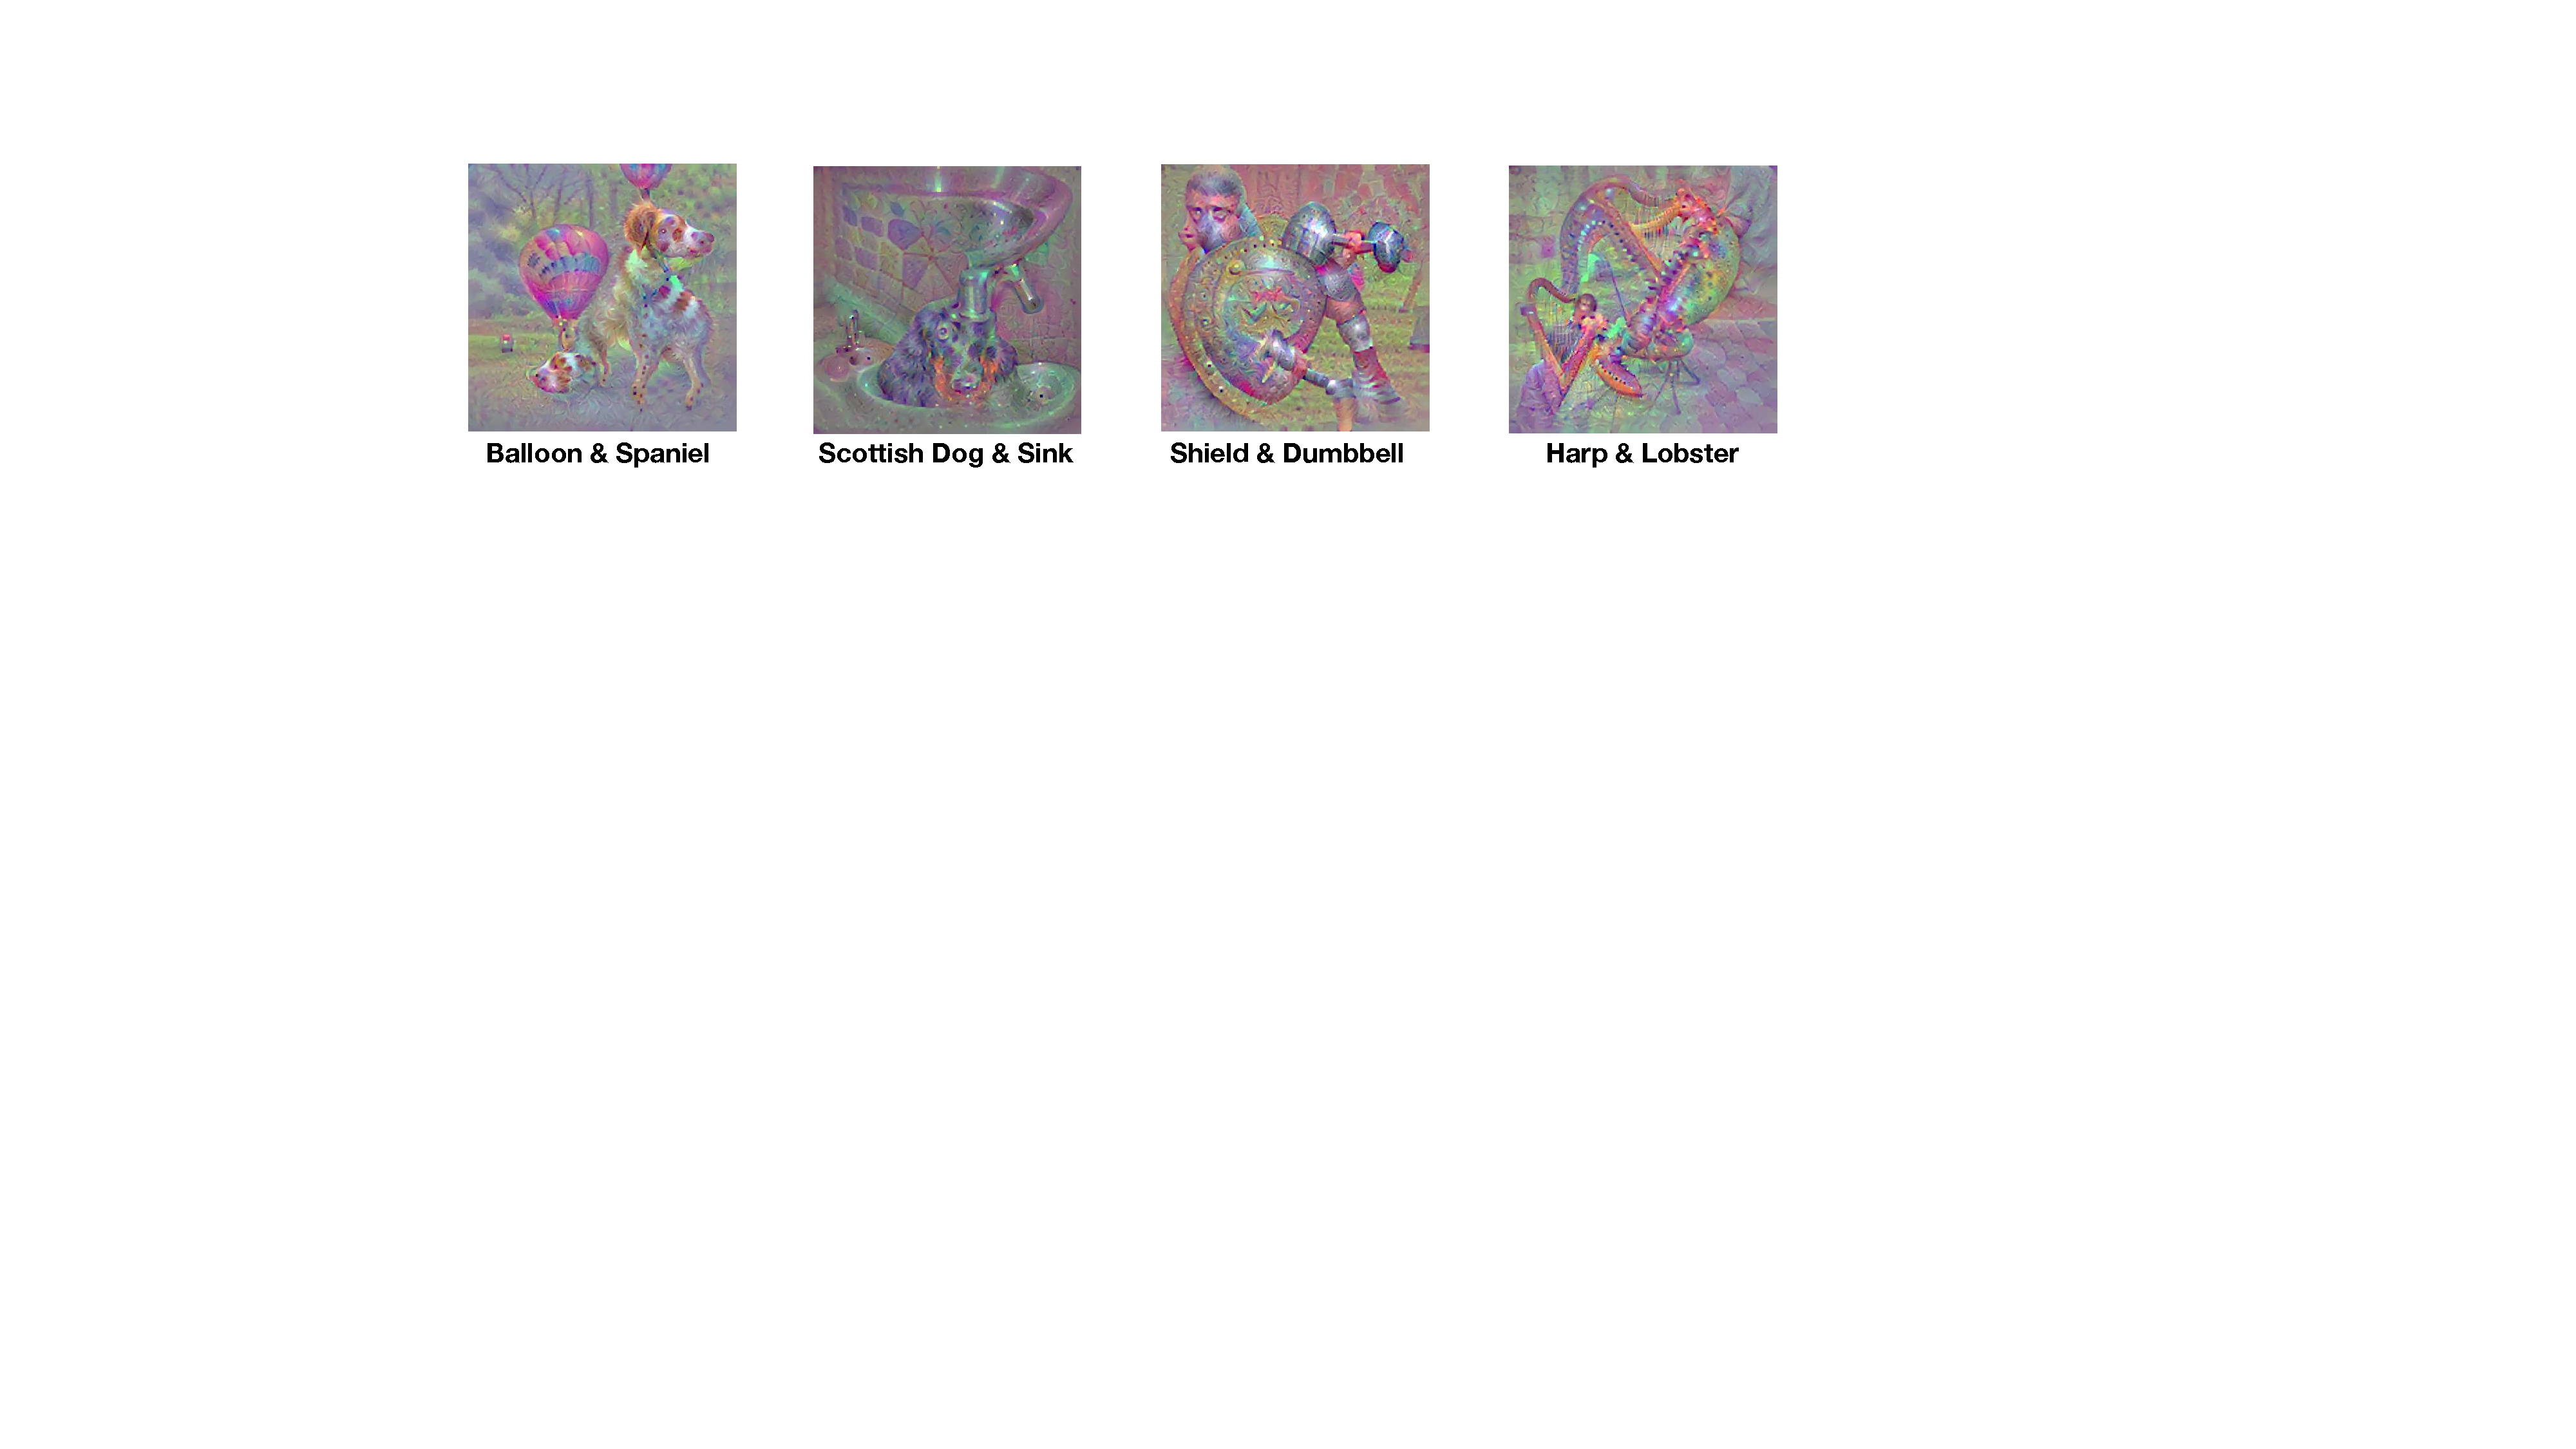
\includegraphics[width=0.8\linewidth]{./figure/mixup_fig_compressed.pdf}
    \label{fig:latent1}
  \end{subfigure}
  \begin{subfigure}[b]{\linewidth}
    \centering
    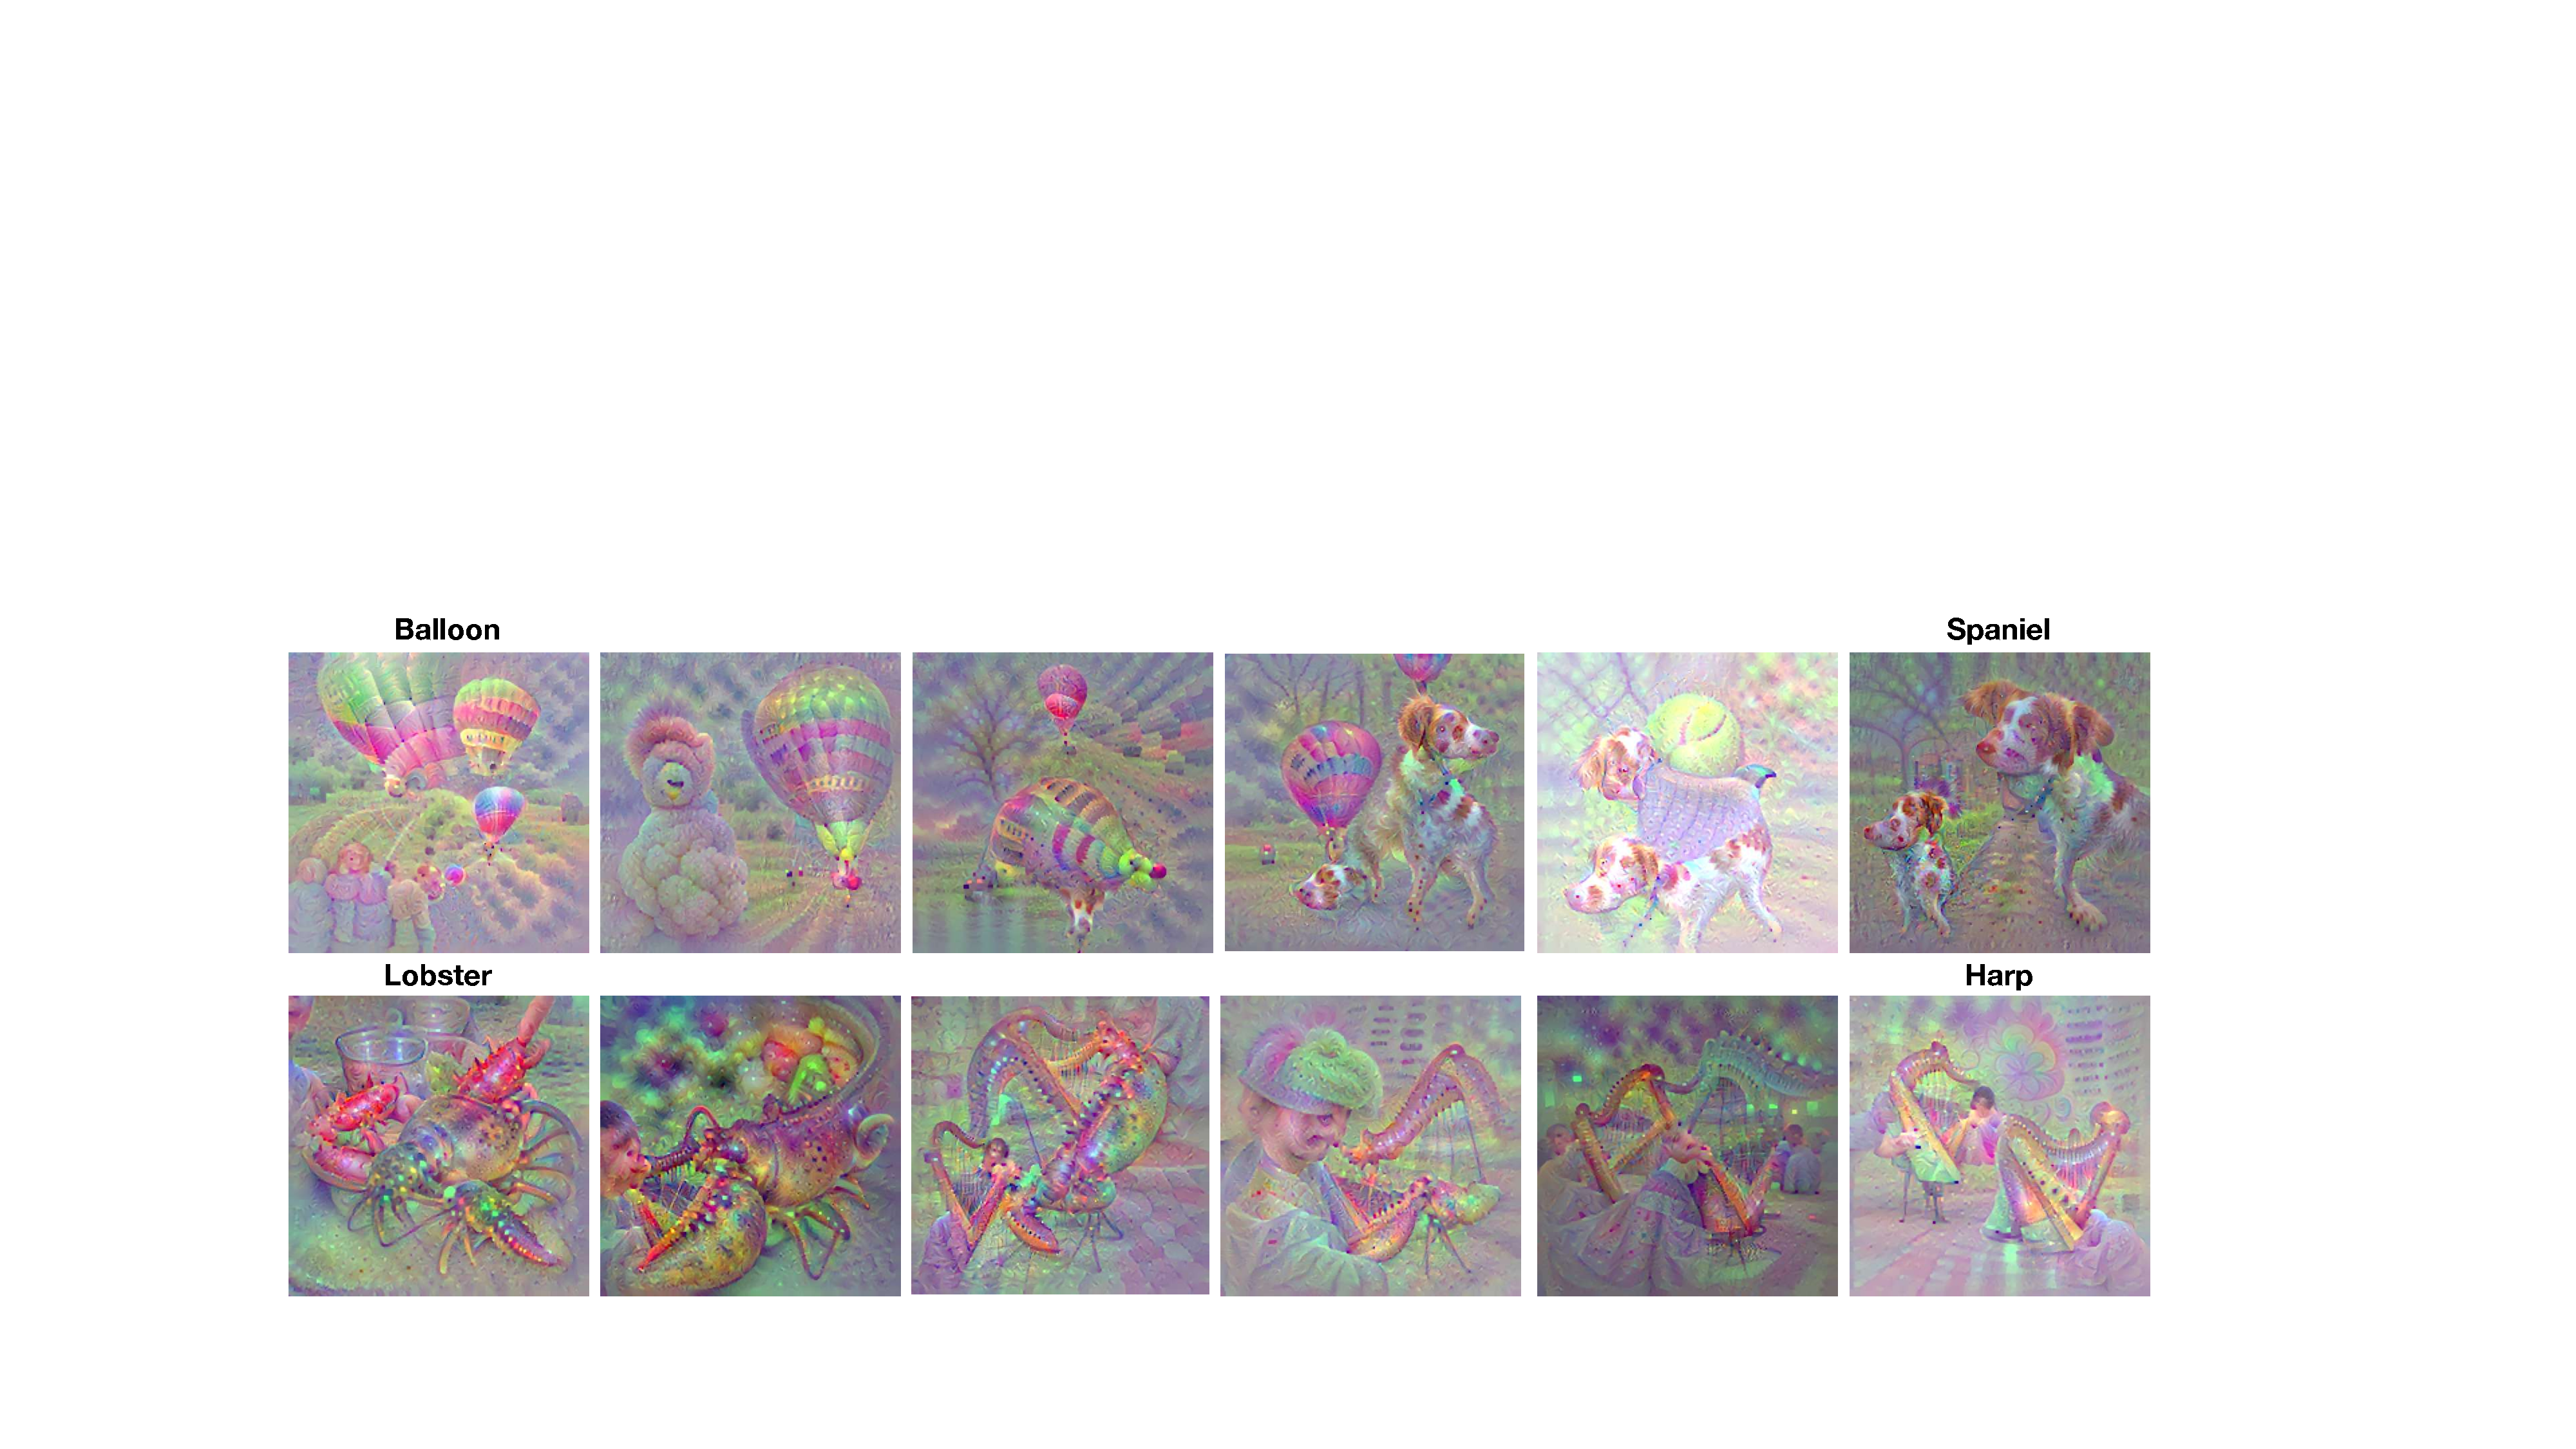
\includegraphics[width=\linewidth]{./figure/interpolation_fig_compressed.pdf}
    \label{fig:latent2}
  \end{subfigure}  
  \begin{subfigure}[b]{\linewidth}
      \centering
    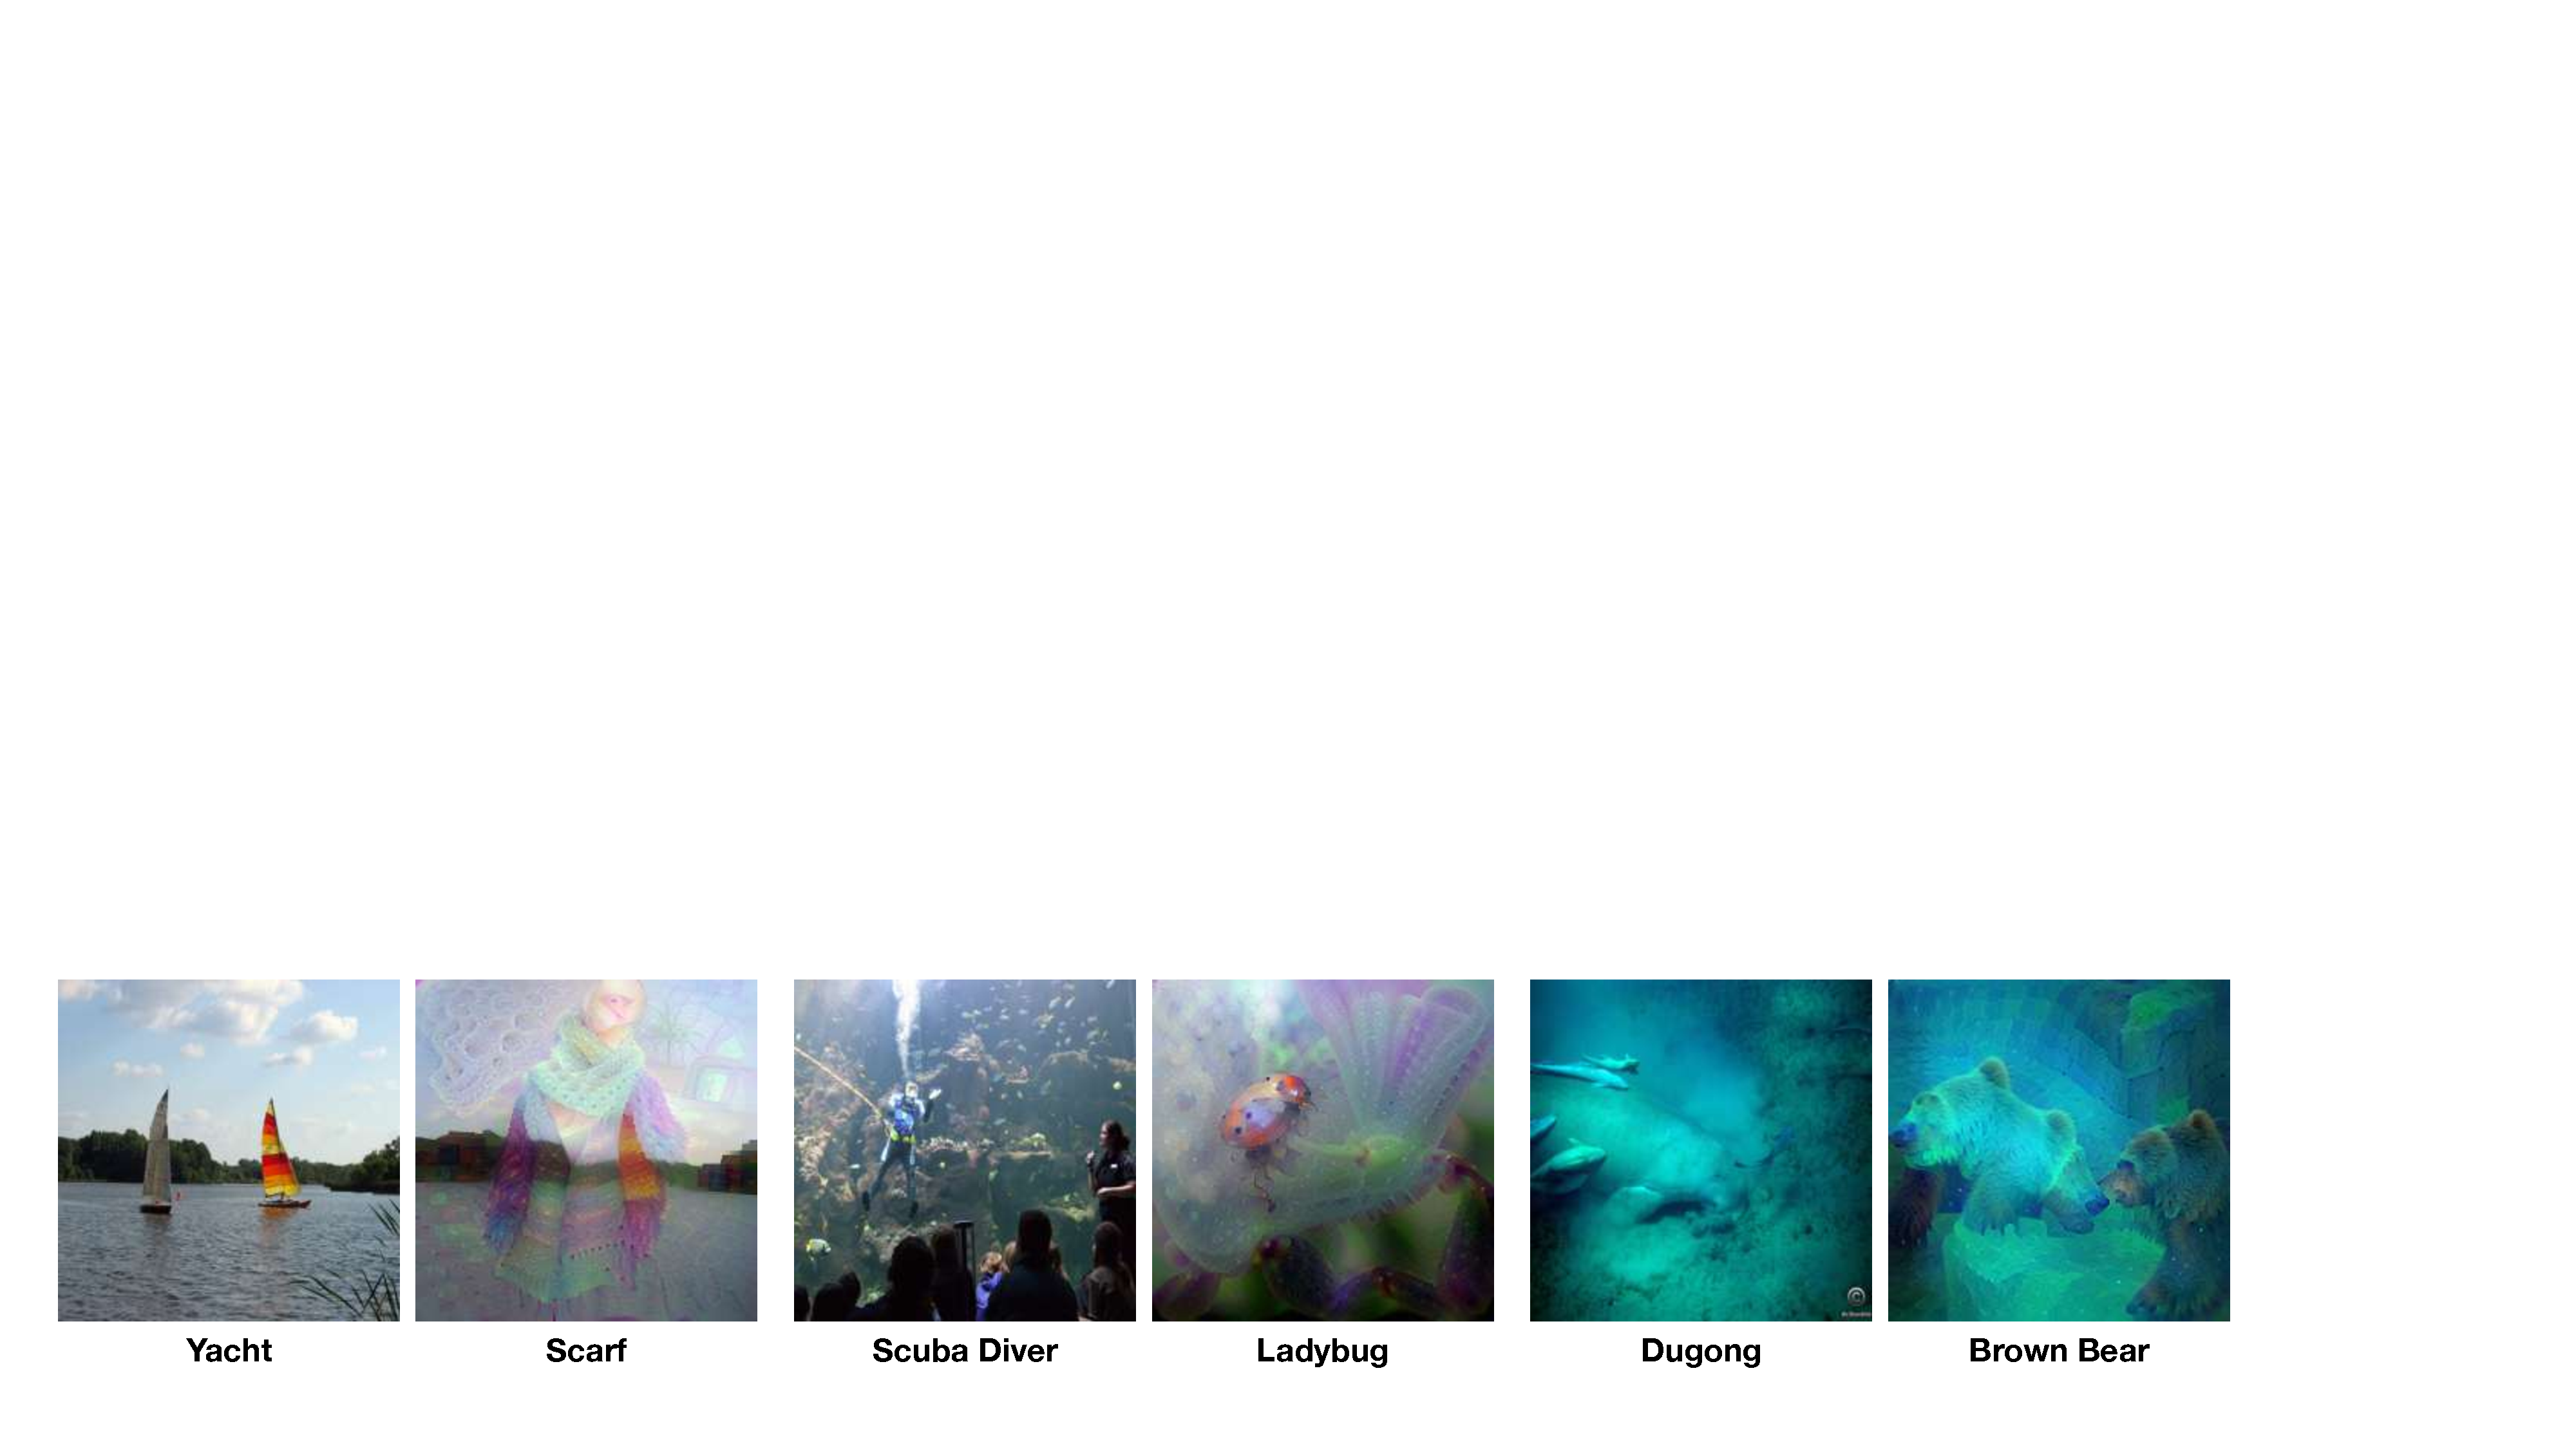
\includegraphics[width=\linewidth]{./figure/mix_imagenet_compressed.pdf}
    \label{fig:latent3}
  \end{subfigure}  
  \caption{\nj{(Top)} \nj{Generated DSVs using} soft labels: $\delta$ was set 0.6, \ie soft label $y = 0.4 y_{\text{left}} + 0.6 y_{\text{right}}$. 
  \nj{(Middle) Examples} of latent (soft-label) interpolation. \jh{(Bottom) Image Editing through latent.}}
  \label{fig:combined}
\end{figure}

\jh{To experimentally verify this, we performed a latent interpolation task and image editing, which is common \nj{in} generative models~\cite{gan1, gan2} By mixing different labels \nj{ (\(y_i = (1-\delta)y_a + \delta y_b\), where \(y_a \neq y_b\)), we generated DSVs as} depicted in Fig.~\ref{fig:combined}. 
%The results \nj{are} astonishing. 
When generating DSVs with these mixed soft labels, \nj{the generated DSVs} semantically represent the midpoint between the two classes. \nj{A generated DSV either simply contains} both images (the case of ``balloon" and ``spaniel") or semantically `fuse' objects (the case of ``lobster" and ``harp", producing an image of a harp made out of lobster claws). 
%For image editing task, similarly, we assigned the latent to desired class. Then, we aligned the image with DeepKKT loss. The result it quite surprising, it successfully transfers image to desired class while maintaining previous images' structure. For example, the sail of the yacht is seamlessly transformed into the shape of a scarf. This task was impossible with other methods; for example, in diffusion models, one would need a mask to seamlessly edit the image.}
\nj{For the image editing task, we assigned the latent variable to the desired class and then aligned the image using DeepKKT loss. The result was quite surprising: the method successfully transferred the image to the desired class while maintaining the original structure. For example, the sail of a yacht was seamlessly transformed into the shape of a scarf. This task was impossible with other methods; in diffusion models, for instance, a mask would be needed to edit the image seamlessly.}
}


The fact that the generated images correctly merge the semantics of the classes suggests \nj{a couple of} significant implications: 1)  1) \jh{\textbf{New Generative Model}: This approach offers a new type of generative model as an alternative to GANs and diffusion models.} It can handle the same task without the need for training a specific model, as it leverages existing classification models for generative purposes. Furthermore, it is lightweight compared to diffusion models.
%\jh{as the alternative for} GANs and diffusion models.
For example, \nj{as the model size of a pretrained ResNet50 for ImageNet is only one-twentieth of that for SDXL~\cite{SDXL}, DSVs show a} potential to leverage existing classification models for generative purposes. 2)  \textbf{Exploration of Classification Model Generalization}: Unlike other generative models, classification models are trained simply to predict the \nj{label} of an image. Yet, in latent interpolation \jh{and editing tasks}, they demonstrate an understanding of semantics. This implies that, despite being trained to memorize class labels, the models grasp the overall semantics of the dataset. As they can generate seemingly unseen samples by interpolation and editing.


% \jh{SVM이 SV인 이유는, support vector를 통해서 우리가 분류 모델을 만들 수 있다는 것이었다. 지금까지 우리는 DSVs와 SV의 등가성에 대해서 다루었고, 실제로 SV가 이론적으로 만족해야 하는 성질을 DSV가 다 만족해야한 다는 것을 보여주었다. 따라서 남은 것은, 바로 DSVs를 통해서 model을 다시 reconstruct할 수 있는지 확인해보는 것이다.}

% \jh{결과적으로 해당 Task가 원하는 것은, model을 학습시키기 위해서 적은 training data를 synthetize 해야 하는, dataset distillation 의 목표와 같아진다. Table.~\ref{table:datasetedistillation}에서 우리는 각 class에 대해서 image를 한 개 만들고, 그리고 이걸 활용해서 scratch에서 retrain하였다. 해당 결과는 기존의 dataset distillation method와 유사한 결과가 나왔는데, 해당 결과는 굉장히 놀라운 결과이며, 기조의 dataset으로부터 coreset selection을 하는 것보다 더 높은 성능을 기록하였다. 이는 적어도 DSVs가 coreset selection을 통해서 dataset에서 고른 것보다 더 높은 성능을 가진다는 것을 방증한다. 또한, 기존의 dataset distillation과 비슷한 성능을 보인다는 것은 굉장히 놀라운 결과이다. 왜냐하면, Sec.에서 설명하였듯이, 기존의 dataset distillation의 경우는 애초에 해당 목표를 성취하기 위해서 meta learning loop를 활용하여서 synthetized data의 gradient가 real dataset과의 gradient와 training model의 trajectory에 일치하도록 하기 때문인데, 이는 수많은 model training, full access of dataset 이 필요한 데 DSVs의 경우는 두개 다 필요하지 않기 때문이다. SVM에서의 support vector처럼 기능하고 있음을 보이며 동시에 기존의, decision criteria를 decoding한다는 것을 방증한다.}

% 위의 두 가지 결과가 암시하는 것은, DSV는 support vector (classical)의 조건을 만족한다는 것과, 그것이 다른 정보에 비해서 정보량이 매우 많다는 것이다. 이 두 가지 결론으로부터 우리는, DSV가 classical Support vector과 같은 역할을 할 수 있다는 것을 알 수 있다. Fig.~\ref{fig:Painting}은 그 주장을 실험적으로 검증하면서도 동시에 DSV의 실천적 활용가능성을 검증하고 있다. 우리는 Fig.~\ref{fig:DSVSET}에서 deer과 cat의 decision criterion에 대해서 다음과 같은 사실을 알고 있다. 1. deer의 DSV의 경우 뿔이 차지하는 비중이 굉장히 클 뿐더러, 해당 요소가 다른 class들과를 구분하는 가장 큰 요소이다. 2. cat의 경우는 굉장히 뾰족한 세모 귀가 고양이를 구분하는 역할을 알 수 있다. 우리는 그 정보를 활용하여서 deer image에서 뿔을 masking하고, 사슴의 귀를 뾰족하게 만들었을 때, 실제 모델이 그 사진을 굉장히 confident하게 고양이인 것으로 인지하고, 사슴의 confident를 극적으로 낮춘 것을 확인할 수 있었다.


% 위 실험과, DeepKKT의 조건을 생각해 보면 DSV는 특수하게 학습되지 않은 일반적인 모델을 Responsible \cite{} 있다는 특성이 잇음을 알 수 있다는 것을 알 수 있는데, 첫째로 DSV는 모델의 decision criteroin을 visaul하게, 사람이 인식가능하게 explain함으로서 우리는 모델이 어떤 방식으로 작동하는지 알 수 있다. 해당 방법론은 기존의 XAI에서 진행된 방법론보다 훨씬 더 광범위하게 적용될 수 있는 방법론이다. 기존의 XAI들이 채택하는 방법론은 gradcam\cite{}와 같은 single input을 설명하는 local explanation 방법론으로서, DSVs와 같이 gloabal한 decision criterion을 보증하지 못한다. 또한, 해당 방법은 model inversion에 기초를 두고 있기 때문에 safe하다. 물론 Fig.~\ref{fig:DSVSET}을 보면, synthetized set의 경우 selected set과 어느종도 비슷하긴 하지만 그것이 실제 샘플과 같은 형상을 띄진 않는 것을 볼 수 있는데, 그 이유는 general한 decision boundary를 인코딩해야 하기 때문에 image-specific한 feature들을 더 담지 않고 있기 때문이다. 따라서 학습과정에서 DSV는 train dataset에 대해서 정보량이 없기 때문에 기존의 generation 방법론보다 헐씬 더 safe하고, privacy issue에서 자유로움을 알 수 있다. 다시 말해서 DSV는 logistic loss를 사용하고 있는 모든 모델들을 적은 computation만으로도 responsible해주게 할 수 있는 특징을 가지고 있다.

% \paragraph{DSV, first measure without scoring}

% 이러한 사실은, 그 뿐만 아니ㅏ라 model의 성능을 측정할 수 있는 질적 요소를 소개한다는 점에서 그 의미가 크다. 예를 들어서 우리가 사슴과 말을 구분해야 하는 class를 풀어야 하고, 이를 위해서 모델을 하나 가져와야 한다고 하자. 만약 이때 우리가 그 데이터를 여름에 수집했다고 할 때 우리는 과연 본 논문에서 사용한 모델을 쓰는 것이 적합할까? 우리는 그것이 아님을 바로 알 수 있다. 왜냐하면, Fig.\ref{fig:DSVSET}는 model이 deer의 판단기준이 뿔에 크게 좌우됨을 알려주기 때문이다! 여름에는 사슴에 뿔이 나지 않는다. 따라서 그 모델은 제대로 classify할 수 있음을 뜻한다.
% 이 함의는 우리는 질적으로 모델을 분석하여 casual prediction을 할 수 있음을 이야기한다. 만약 우리가 DSV를 사용하지 않는다면, 우리는 절대적으로 그 판단기준을 score에 대해서 의존해야 한다. 이는 굉장히 위험한 선택이다. 가령 왜냐하면 모델의 성능은 극히 데이터에 의존하며, 만약 데이터가 오염되었다면 (backdoork atack)거나, 혹은 인종편향되었다면 모델은 제대로 된 판단을 하지 못하기 때문이다. 예를 들어 흑인과 고릴라 사례 (그런데 이걸 넣을지 말지는 모르겠어)를 들 수 있으며, DSV는 우리를 그런 위험성으로부터 예방한다.


% \subsection{Primal condition as an classifier guidence}

% \subsection{DSVs for harsh condition}




% \subsection{Primal condition, as an guidence of DSVs}\label{sec:diffusion}

% \hh{As described in Sec.\ref{sec:DKKTcondition}, the primal feasibility condition plays a critical role in ensuring the model correctly classifies its DSVs, while the stationary condition drives the DSVs towards the decision boundary. Fig.\ref{fig:primalstat} presents the results of extracting DSVs using solely either the primal or the stationary condition for the classes cat and deer. It is observed that using only the primal condition captures global features such as textures necessary for classification, whereas the employment of the stationary condition alone results in the extraction of features resembling actual dataset characteristics, like shape and edge details. Since the stationary condition does not directly reflect class constraints, it generates artifacts similar to the dataset but fails to make class-specific adjustments, leading to a notable decrease in model accuracy for those samples. Therefore, it becomes evident that the primal condition, in its role as a classifier guidance, is crucial in the extraction process of DSVs. Moreover, akin to typical generative models utilizing classifier guidance, an appropriate interpolation between the two losses can be employed to modulate classifier guidance, enabling sampling in a manner similar to generative models.}



% 지금까지는 DSV들은 세가지 DKKT 조건들을 정확하게(implicit)하게 만족하도록 constraint들을 주었다. 하지만 모든모델들이 overparameterized, overfitting된 세팅에서 학습된것이 아니며, 현재 practical 하게 많이 쓰이는 Test Time Adaptation 이나 domain generalization과 같은 setting에서는 test time에서 완전히 converge된다는 보장이 없다. Fig 7에서는 CIFAR-10 dataset에 대해서 학습한 encoder을  가지고 SVHN dataset으로 transfer learning을 진행하여 학습된 마지막 몇개의 layer에 대해서 DSV들을 뽑은 artifact들이다. 이때 SVHN dataset에 대하여 training accuracy가 80$\%$ 임에도 불구하고(primal condition을 완전히 만족하지 못하는 환경에서도) 효과적으로 해당 데이터셋의 feature들을 잘뽑아냄을 확인할 수 있다. 이를 통해서 1. 다른 데이터셋에 편향되어 되어있는 top layer 뒤에 일부 layer만 학습시켜도 DSV를 독립적으로 뽑을 수 있다는점 2. training accuracy가 100$\%$가 아닌 relaxed, practical 한 industry 환경에서도 robust하게 적용할 수 있다는 점을 확인할 수 있었다. 
% 1. Transfer니까 좀 특이함. 2. practical한 이유가 그 대부분 모델은 top layer만 쓰고, 그리고 적은 layer로도 된다는걸 보여줌 -> computation cost 더 줄일 수 있는 가능성 좀재. + 실제로 이거 accuracy 100퍼 안되는 (어떻게 보면 overparameterized 안되는) 상황에서도 잘 됨.


% Figure X indicates .. Also , 

% \subsection{Reverse Engineering}
% \subsection{Deep Support Vector Selection}

% \subsection{Role of each loss, in the aspect of dataset distillation}





% Primal 만 썼을때의 양상과, stationarity만 썼을때의 양상 차이 texture vs shape 다만 실제로 stationarity만 했을 때에는, accuracy 보정이 되지 않기 때문에 accurarte하게 estimate하지 않은 것들의 경우는 제대로 나오지 않는다. 각각 cat, deer

% \begin{figure}[t]
%   \centering
%    \includegraphics[width=0.8\linewidth]{./figure/lambda_diff.pdf}
%    \caption{selection 한 것과, synthethis 한 것이 lambda의 상대적 값에 따라서 비슷하게 간다는 것을 보여주는 사진}
%    \label{fig:lambda_diff}
% \end{figure}

% \subsection{Transfer Learning에서 SVM 만들기 (이건 오늘 하자)}

% \subsection{Dataset Condensation}

% Our algorithm fundamentally defines and seeks deep support vectors (DSVs), which are the backbone of the model. \hh{Considering} that the number of DSVs is substantially smaller than the entire dataset, our approach can naturally be considered a dataset distillation problem. \cite{}

% The primary goal of dataset distillation is to enhance privacy and reduce communication load by creating a smaller dataset that retains equivalent performance to the original dataset \hh{via} gradient matching\cite{}. It involves using the original dataset to generate hundreds of models\cite{}, or in other words, to minimize the gradient difference when the original data \( x \) and the distilled data \( \tilde{x} \) are fed forward through the trained model \( \theta \). This process necessitates high computational cost due to the use of the entire dataset and even requires the Hessian when trajectory matching is performed \cite{}. Those requirements imply that conventional dataset distillation algorithm should be performed in central node which can process high-order computation and memory cost algorithm. \hh{However the process of centralizing data processing creates a challenging situation, as the data comes from edge devices like smartphones. Moving raw data from these devices to a central system ends up causing the privacy and communication issues that dataset distillation is supposed to solve. Therefore, the solution to dataset distillation needs to happen on the edge devices, without the need to send out the training data.} 
% % However, this centralized processing leads to a paradoxical situation because the data is obtained from edge devices like smartphones. That is, transferring raw data from edge devices to the central node itself brings the very privacy and communication burden issues that dataset distillation aims to resolve. Thus, the dataset distillation problem must be resolved at the edge device without training data.

% \hh{이텔릭이나 headings로 조건들 나열하기}
% However, storing the entire dataset at the edge is impractical due to the significant computational burden involved in gradient matching. Moreover, the continuous learning setting, often presupposed at the edge, cannot be accommodated due to these constraints. Holding data for gradient matching introduces privacy risks, akin to those in other generative models, and these are not fully alleviated even when datasets are synthesized using GANs trained with the original dataset.

% In contrast, our DSV methodology inherently overcomes these issues. \hh{Our algorithm, which does not require any access to training data, could provide a viable solution to privacy concerns. Moreover, the computational cost of this approach is on par with that of initial model training. In the perspective of the resolution on DSVs, results[?] indicate a significant advantage in that our method can achieve comparable performance even with low-resolution DSVs. Furthermore, this approach allows for a flexible trade-off depending on computational resources: lower resolution DSVs can be employed in scenarios with limited computational capacity, while higher resolution DSVs can be utilized in edge devices with more computational leeway. This flexibility in managing the trade-off between DSV resolution and computational demand constitutes a key strength of our methodology.} 
% Our approach is pioneering in that it resolves this issue by employing updates that rely solely on DSVs, which substantially diminishes the computational load. This innovative method renders dataset distillation a viable and practical solution within edge computing paradigms.


% \jh{TODO experiments: 9:18 PM 이준후 Application to non classification methods}








% \jh{여따가 lambda의 역할을 넣는것도 괜찮을 것 같다. lambda가 큰 figure, lambda가 작은 figure, lambda별로 값.}
% \jh{여따가 Primal과 stationarity의 역할을 넣자. Primal의 역할, stationarity의 역할...}



% \subsection{Adversarial Attack}
% \hh{ In adversarial attacks, the objective is to perturb the model by adding noise of minimal epsilon magnitude. This strategy often exploits the fact that misclassifications commonly occur near the decision boundary, allowing for the effective creation of adversarial examples using Deep Support Vectors (DSVs) close to this boundary. As depicted in Fig.~\ref{fig:adversarial}, even a minimum addition to an image labeled 'dog'—merely 1\% of the size of the 'dog' image—can lead to its misclassification by the model. When crafting adversarial examples, it's crucial to minimally alter the original image while navigating the semantic space. DSVs, possessing high-quality semantic information in the decision boundary space, enable slight modifications without significant distortion of the original image, effectively disrupting the model. \\ To counteract adversarial attacks, training with a diverse range of augmented images is essential. However, there typically exists a trade-off between generalized clean accuracy and robust accuracy; i.e. training with various augmentations might enhance robustness but detrimentally affect clean accuracy (proper evaluation of original images). Therefore, efficient augmentation is necessary. Leveraging the insight that adversarial examples are primarily generated near the decision boundary, the extracted DSVs can be simply combined for augmentation in training. The method of extracting DSVs is not only computationally light but also efficient and straightforward in its augmentation approach, making it potentially effective against general adversarial attacks.}





% adverserial attack에서는 최대한 작은 입실론의 크기의 노이즈를 첨가하여 모델을 교란시키는 것이 목적이다. 주로 decision boundary에서 오분류가 많이 일어난다는 사실을 이용하여 decision boundary에 가까운 DSV들을 통하여 adverserial example들을 효과적으로 만들 수 있다. FIG 8에서는 'dog' 라벨의 이미지에 크기가 매우 작은 ('dog' 이미지의 1$\%$ 크기)를 추가하였는데 모델이 분류함을 알 수 있다. adverserial example을 만들때는 원본사진을 최대한 훼손하지 않으면서 semantic공간에서의 이동이 필요한데, DSV들은 decision boundary space에서의 질높은 semantic정보를 가지고 있어서 조금의 첨가만으로도 원본 이미지를 훼손하지 않는 선에서 모델을 효과적으로 교란시킴을 확인할 수 있다.
% Adverserial attack 에 대응하기 위해서는 다양한 augmented image들에 대한 학습이 필요하다. 하지만 일반적으로 generalized clean accuracy와 robust accuracy간의 차이가 있다; i.e. 다양한 augmentation들로 학습하는것이 robustness에는 좋을지 몰라도 clean accuracy입장에서는 안좋은 trade off(원본 이미지에 대한 제대로된 평가)가 발생하기때문에 효율적인 augmentation이 필요하다. Adverserial examples들이 주로 decision boundary에 주로 생성된다는 것을(cite) 이용하여 추출된 DSV들을 단순히 합하여 augmentation을 해서 학습할 수 있다. DSV를 추출하는 방법의 computation cost가 가벼울 뿐만 아니라 augmentation 방식 또한 효율적이면서 간단하여 general한 adverserial attack 대비에 효율적일 것이다. 

% 보안에서의 필요성 $\rightarrow$ 오뷴류를 이용하여 이익 얻을 수 잇음  robustness, generalization

% clean accuracy와 robust accuracy간의 차이가 있음-> 따라서 별의별 augmentation들로 학습하는것이 robustness에는 좋을지 몰라도 clean accuracy입장에서는 안좋은 trade off(원본 이미지에 대한 제대로된 평가)가 발생하기때문에 효율적인 augmentation이 필요하다. + 특정 공격에 overfitting
% adverserial examples들은 주로 decision boundary에 주로 생성되며(servay 논문)  